\documentclass{beamer}
\usepackage{ctex}
\usepackage{booktabs}
\usepackage{multirow}
\usepackage{upgreek}
\usepackage{textpos}
\usepackage{tikz}
\usepackage{bm}
%这一句应用PPT的模板,现在有几种可选。
% beamer有Warsaw,Madrid,Pittsburgh,Rochester,等以城市命名的若干模版
% 这些模板的式样可以在/usr/share/texmf/doc/latex/beamer目录中找到相应的例子,
% 根据例子选择合适的模版即可
\usetheme{Warsaw}
\setbeamercovered{transparent}
%\setbeamersize{text margin left=30mm,text margin right=30mm} 
%\usecolortheme{lily}
%\logo{
\includegraphics[scale=0.1]{QSY.eps}}
%\title{硅基混合集成自脉冲\hspace{0em}DFB\hspace{0em}激光器及其应用研究}
\title{硅基混合集成自脉冲\mbox{DFB}激光器及其应用研究}

\author[Centre for Optical and Electromagnetic Research]{答辩人:马珂奇\texorpdfstring{\\[1ex]指导老师:何赛灵\hspace{0.5ex}教授}{}}

\date{2019年6月13日}

% 这个地方对颜色进行设置,设置题目的颜色是80%的黑色混合20%的黑色
%\setbeamercolor{title}{fg=red!10!black}

\begin{document}
\begin{frame}
\titlepage
\end{frame}

\begin{frame}
\frametitle{目录}
\tableofcontents
\end{frame}

\section{研究背景}
\frame{\tableofcontents[currentsection]}
\begin{frame}{研究背景}
\centering
\begin{tikzpicture}
\node[anchor=south west,inner sep=0] (image) at (0,0) {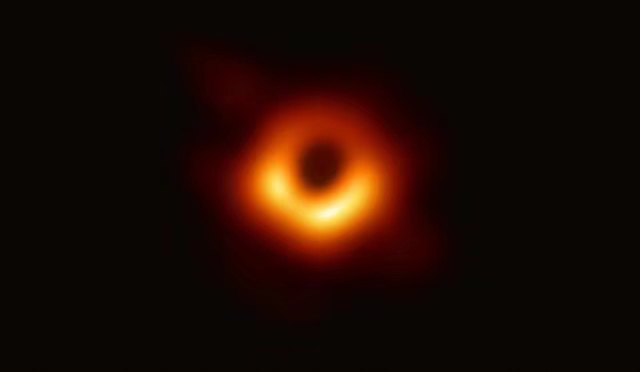
\includegraphics[width=0.95\textwidth]{../Pictures/intro_black_hole.jpg}};
\begin{scope}[x={(image.south east)},y={(image.north west)}]
%\draw[help lines,xstep=.1,ystep=.1] (0,0) grid (1,1); %参考线绘制
%\node[anchor=south east,inner sep=0] at (1,0) {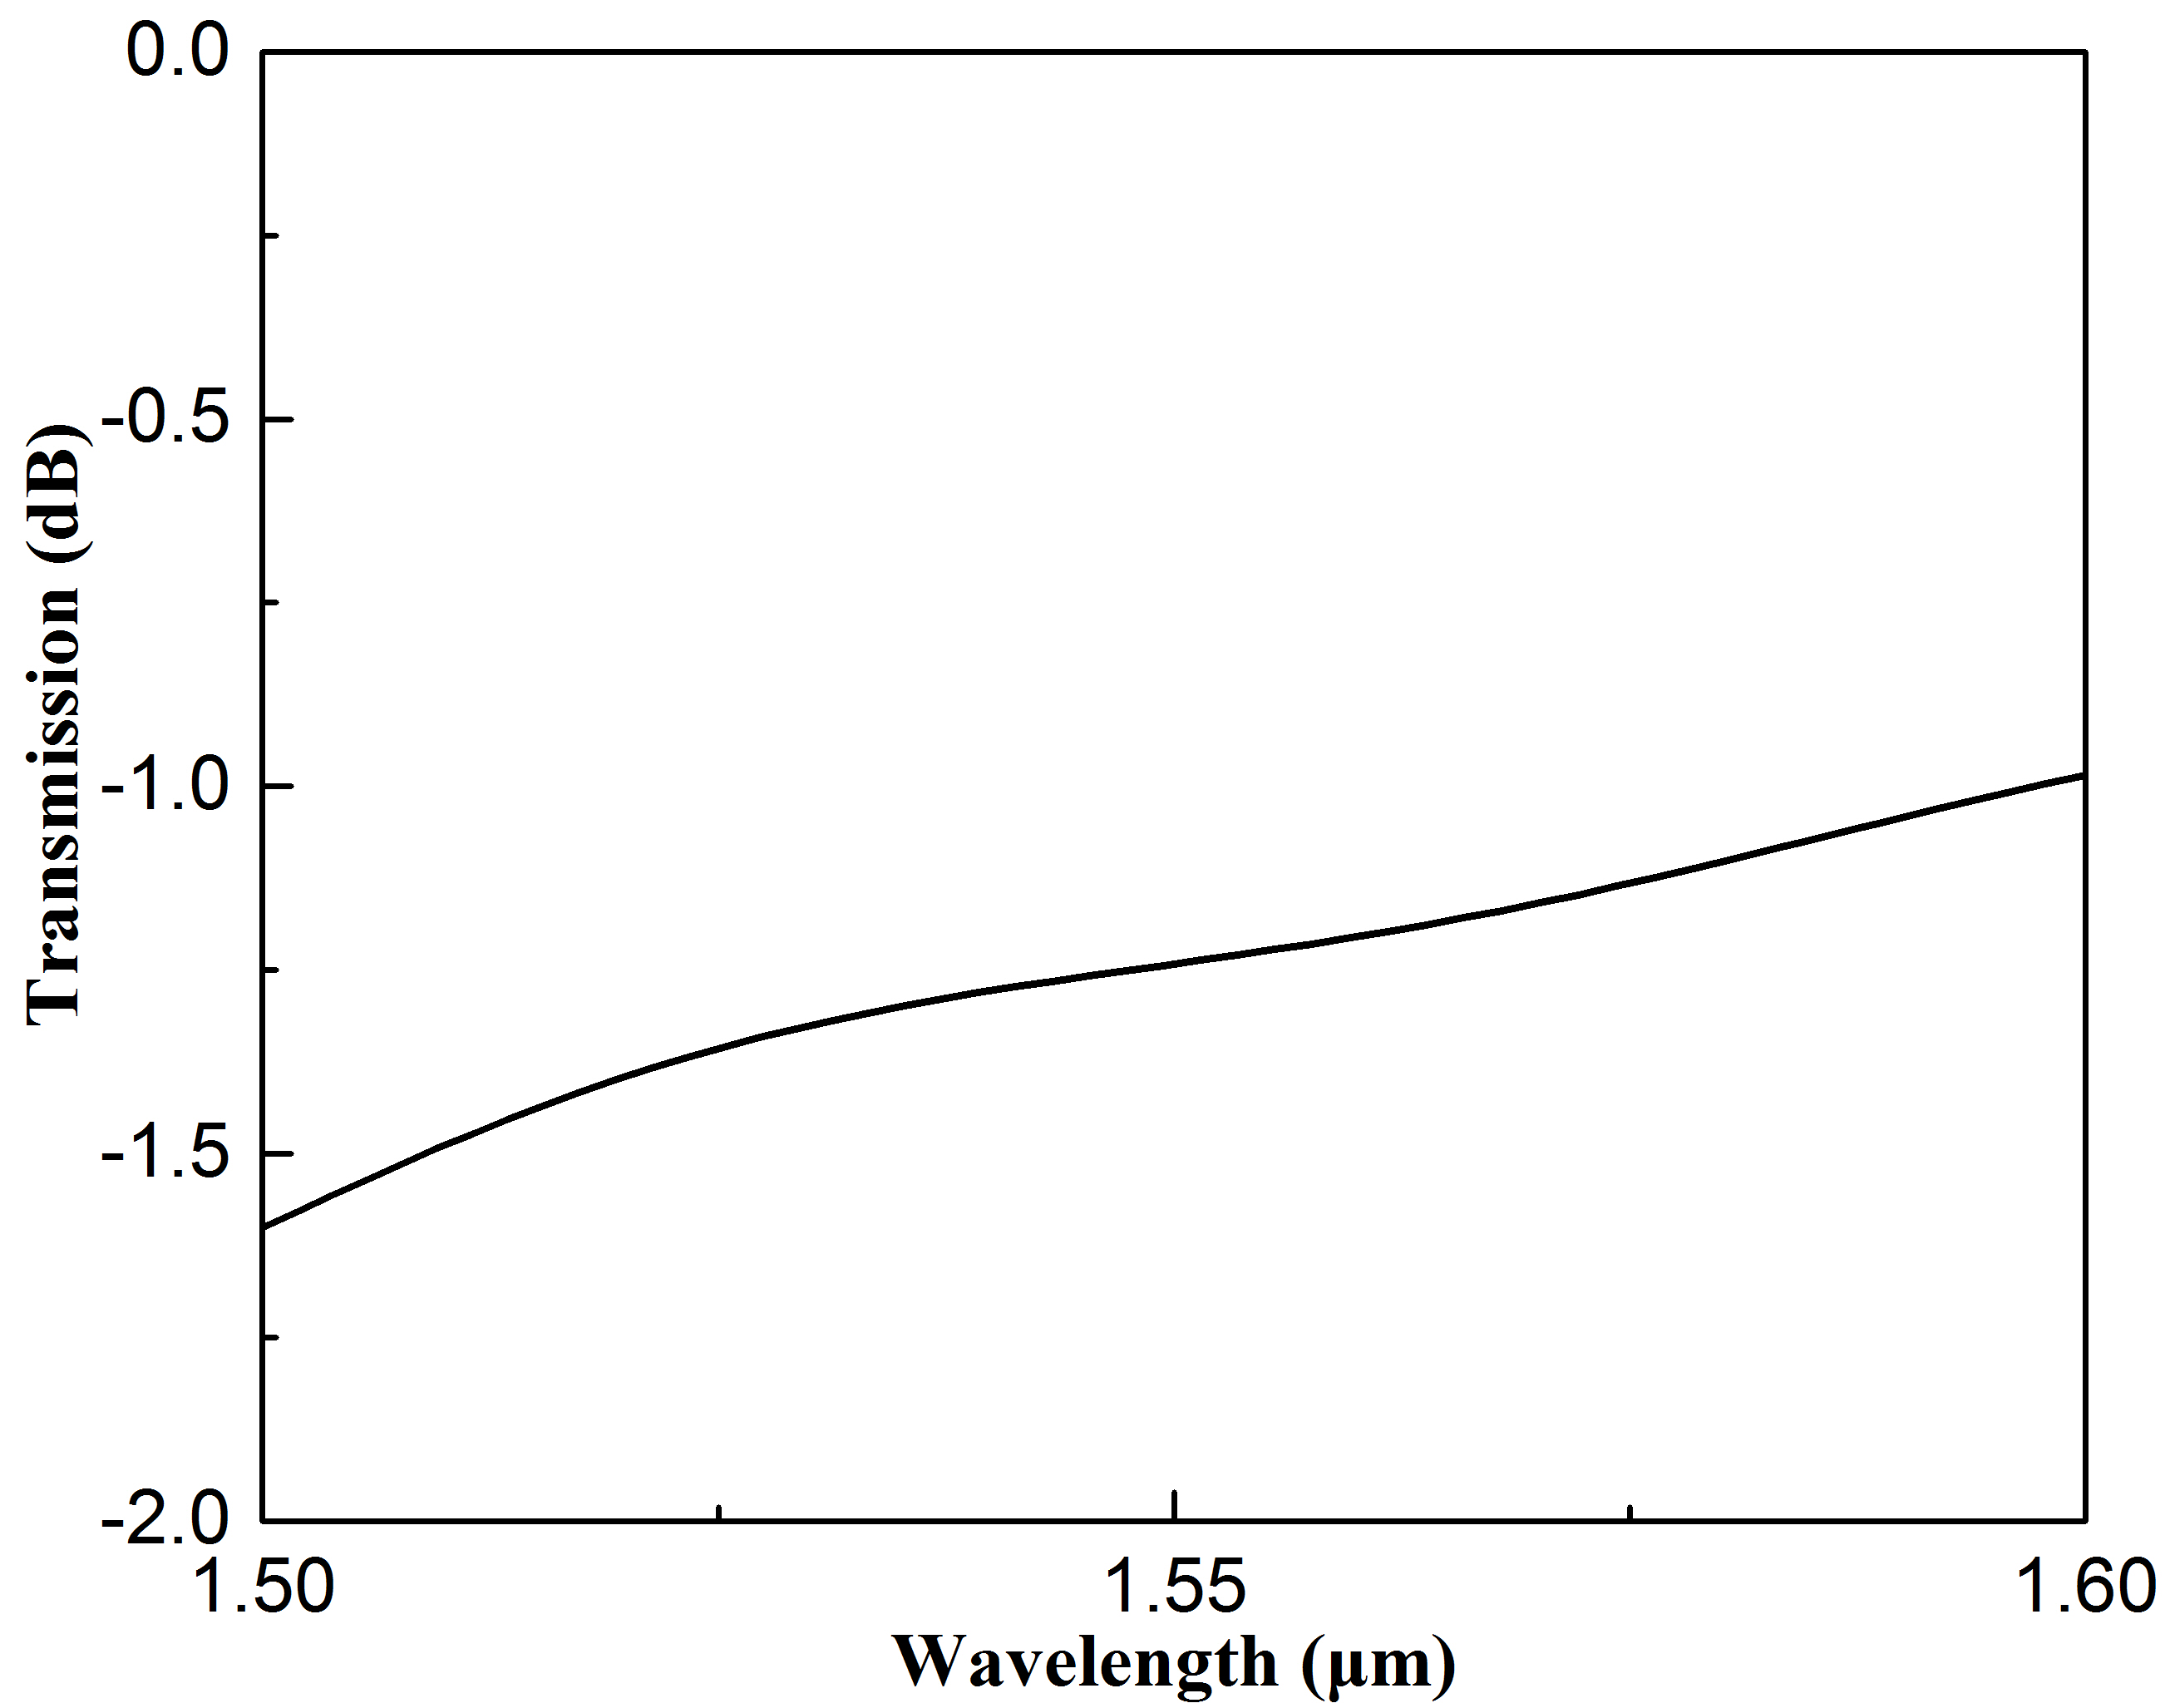
\includegraphics[width=0.27\textwidth]{../Pictures/edg_dbr_loss.jpg}};
%\node[anchor=center,inner sep=0] (A) at (0.52,0.5) {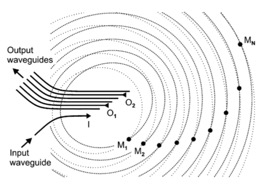
\includegraphics[width=0.32\textwidth]{./Pictures/twostigmaticpoints.jpg}};
%\node[anchor = south east,inner sep=0,font=\tiny, scale =0.8] at (A.south east) {\bfseries \emph{Horst F., Photon. Technol. Lett. 21(23)}};
	\only<1>{\node[anchor = south,white,draw,font=\bfseries] at (0.5,0) {\zihao{6}人类首张黑洞照片};}
	\only<2>{\node[anchor = north west,align = left,white,draw,font=\bfseries] (text1) at (0,1) {海量数据\\2017年:10 PB};
			 \node[anchor = center,inner sep=0,yshift=-0.5cm] at (image.center) {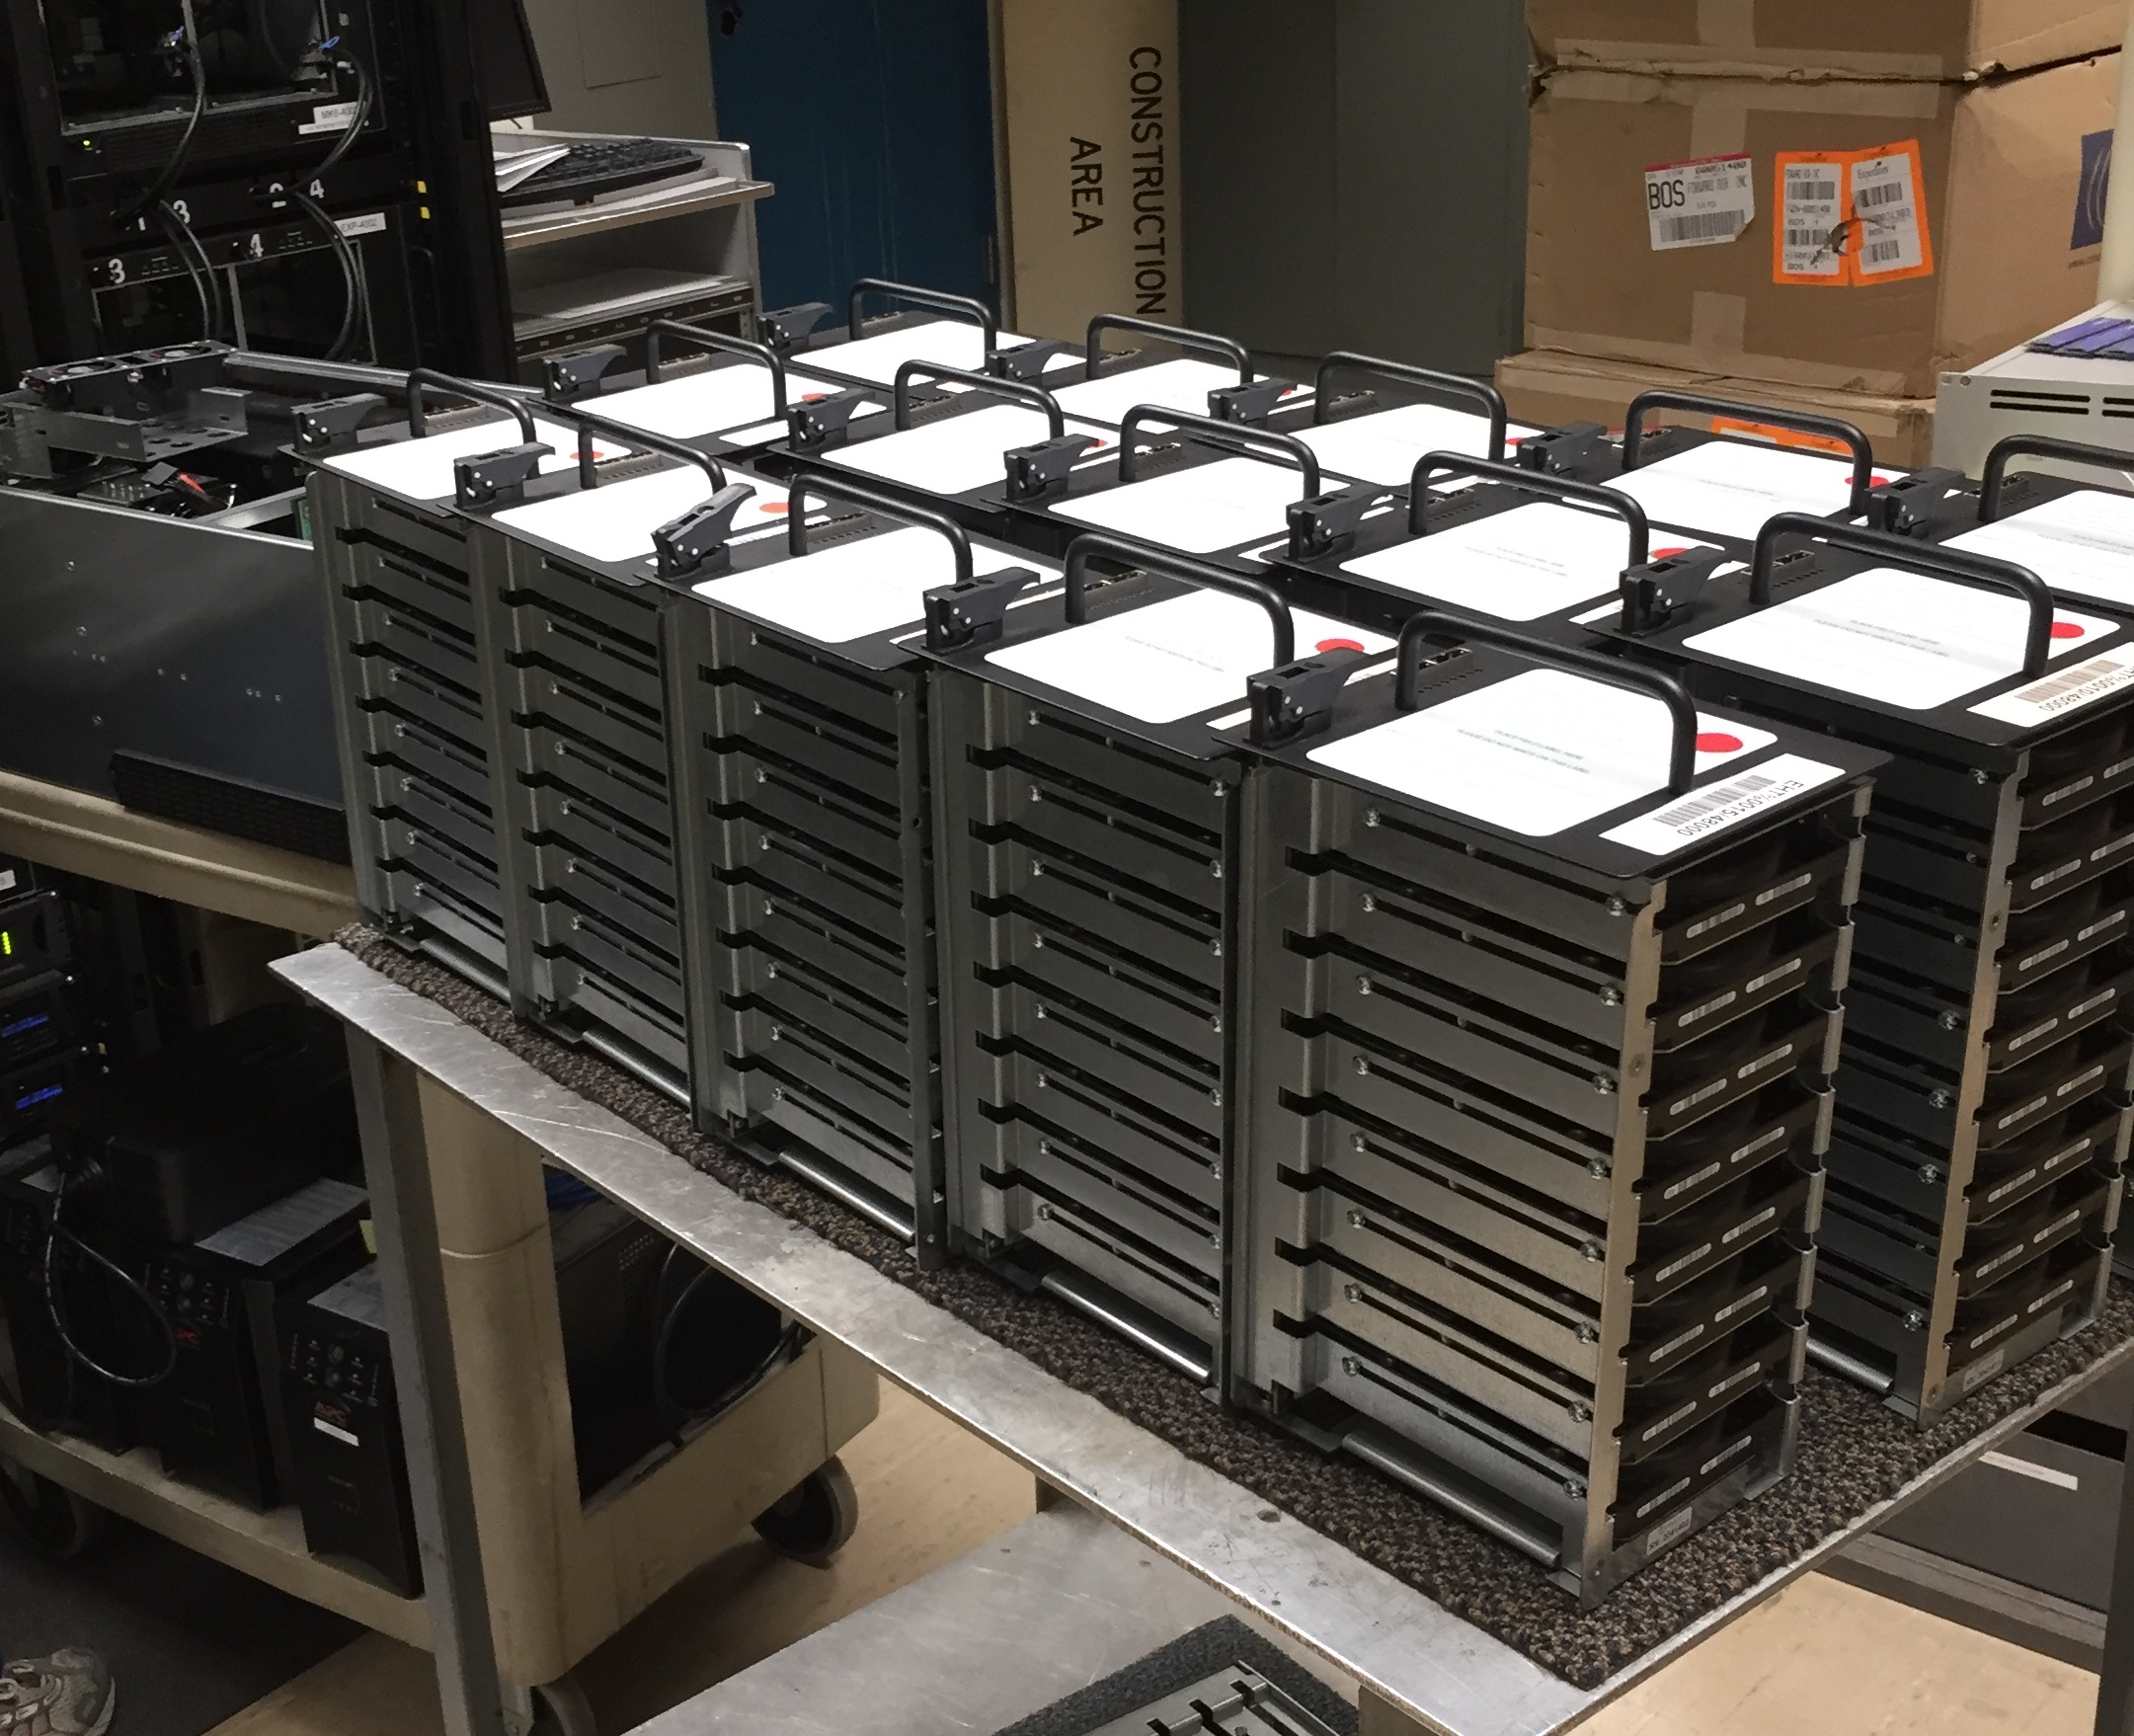
\includegraphics[width=0.5\textwidth]{./Pictures/spt_data_delivery_2017_4.jpg}};}
	\only<3>{\node[anchor = center,inner sep=0,yshift=0cm] at (image.center) {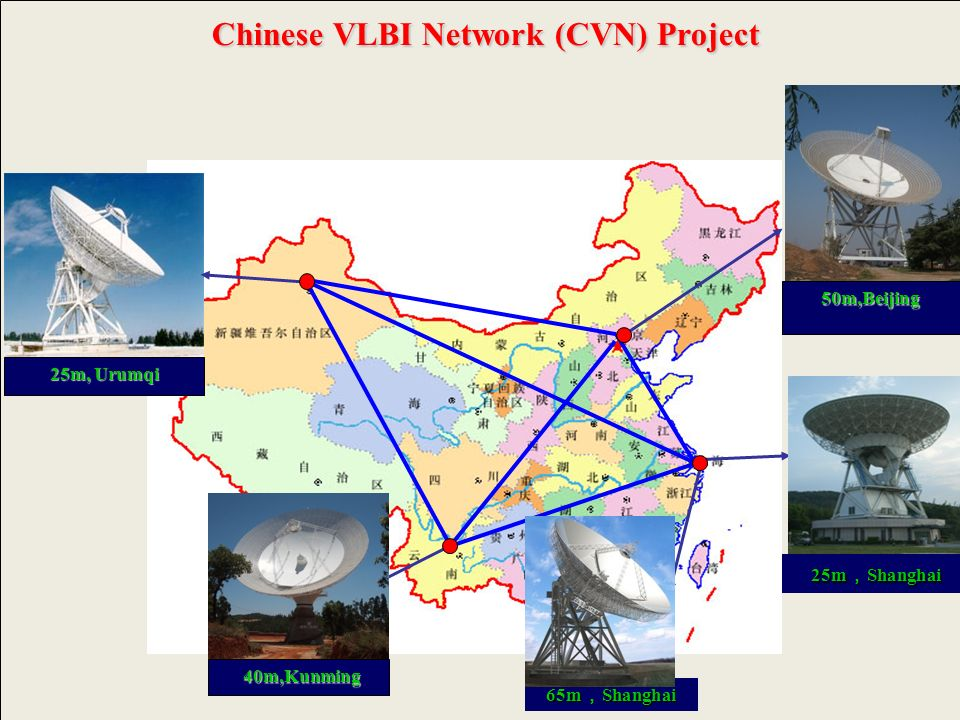
\includegraphics[width=0.7\textwidth]{./Pictures/chinavlbi.jpg}};}
	\only<4>{\node[anchor = north,align = left,white,draw,font=\bfseries] (text1) at (0.5,1) {中国下一代互联网\mbox{(CNGI)}};
		     \node[anchor = center,inner sep=0,yshift=-0.5cm] at (image.center) {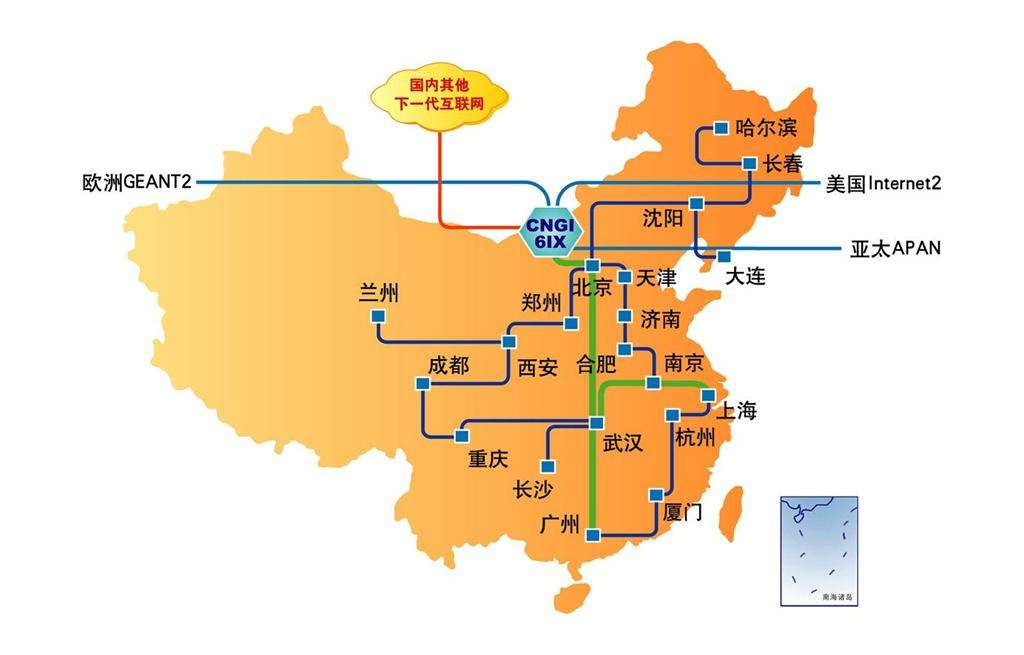
\includegraphics[width=0.7\textwidth]{./Pictures/cngi.jpg}};}
\end{scope}
\end{tikzpicture}
\end{frame}

\begin{frame}{研究背景}
\centering
\begin{tikzpicture}
\node[anchor=south west,inner sep=0] (image) at (0,0) {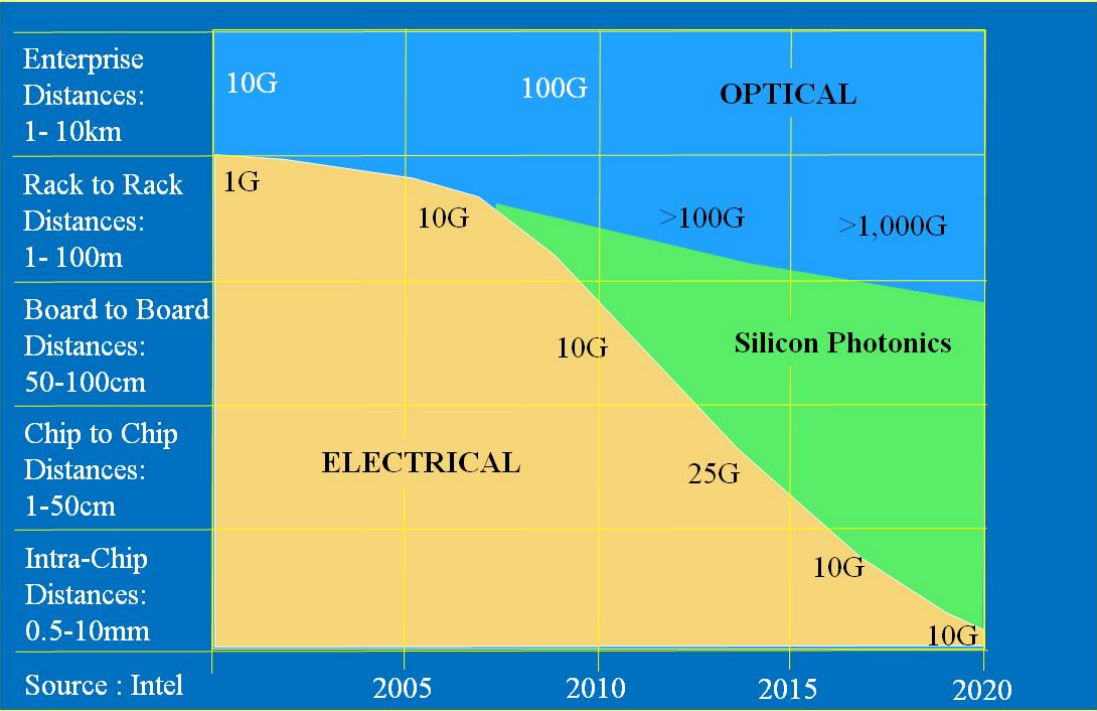
\includegraphics[width=0.65\textwidth]{../Pictures/intro_siliconphotonics.PNG}};
	\begin{scope}[x={(image.south east)},y={(image.north west)}]
		%\draw[help lines,xstep=.1,ystep=.1] (0,0) grid (1,1); %参考线绘制
		\node[anchor = north west,inner sep=0](transceiver) at (1.02,1) {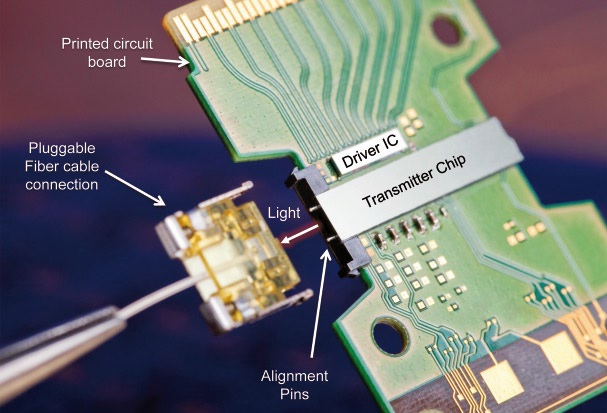
\includegraphics[width=0.32\textwidth]{./Pictures/inteltransceiver.jpg}};
		\node[anchor = north east,inner sep=0] at (transceiver.south east) {\bfseries\tiny \emph{Mario J., Optik \& Photonik, 6(2)}};
		\node[anchor = south west,inner sep=0](mitchip) at (transceiver.west|-{(0,0)}) {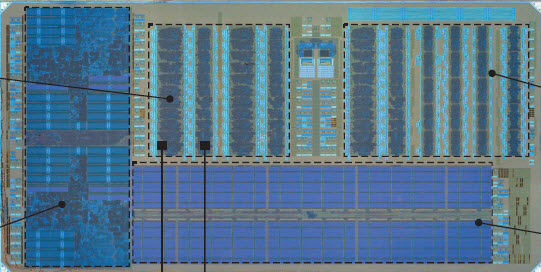
\includegraphics[width=0.32\textwidth]{./Pictures/mitibmchip.jpg}};  %tranceiver的坐标还是图片的中心的坐标,而不是左下角的坐标,加上.west后解决问题 19-06-11,答辩前2天。
		\node[anchor = north east,inner sep=0](text) at (mitchip.south east) {\bfseries\tiny \emph{Sun C., Nature, 528(7583)}};
		\draw [ultra thick,red,arrows=-{stealth},inner sep=4pt] (0.9,0.5) -- (transceiver.west);
		\draw [ultra thick,red,arrows=-{stealth},inner sep=4pt] (0.9,0.35) -- (transceiver.west);
		\draw [ultra thick,red,arrows=-{stealth},inner sep=4pt] (0.9,0.35) -- (mitchip.west);
		\draw [ultra thick,red,arrows=-{stealth},inner sep=4pt] (0.9,0.18) -- (mitchip.west);
	\only<2,3>{\fill [draw=none, fill=white, fill opacity=0.9] (image.north west) -- (transceiver.north east) -- (text.south east) -- (image.south west|-text.south) -- (image.north west) -- cycle;
		\node[anchor = center,inner sep=0] at (0.75,0.5) {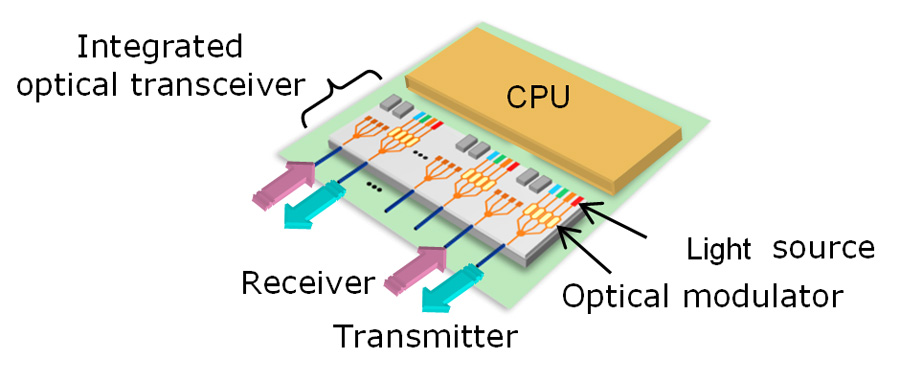
\includegraphics[width=0.7\textwidth]{../Pictures/intro_transceiver.jpg}};}
	\only<3>{\draw[red,ultra thick,rounded corners] (1,0.35) rectangle (1.29,0.45);}
	\end{scope}
\end{tikzpicture}
\end{frame}

\begin{frame}{研究背景}
\centering
\begin{tikzpicture}
\node[anchor=south west,inner sep=0] (image) at (0,0) {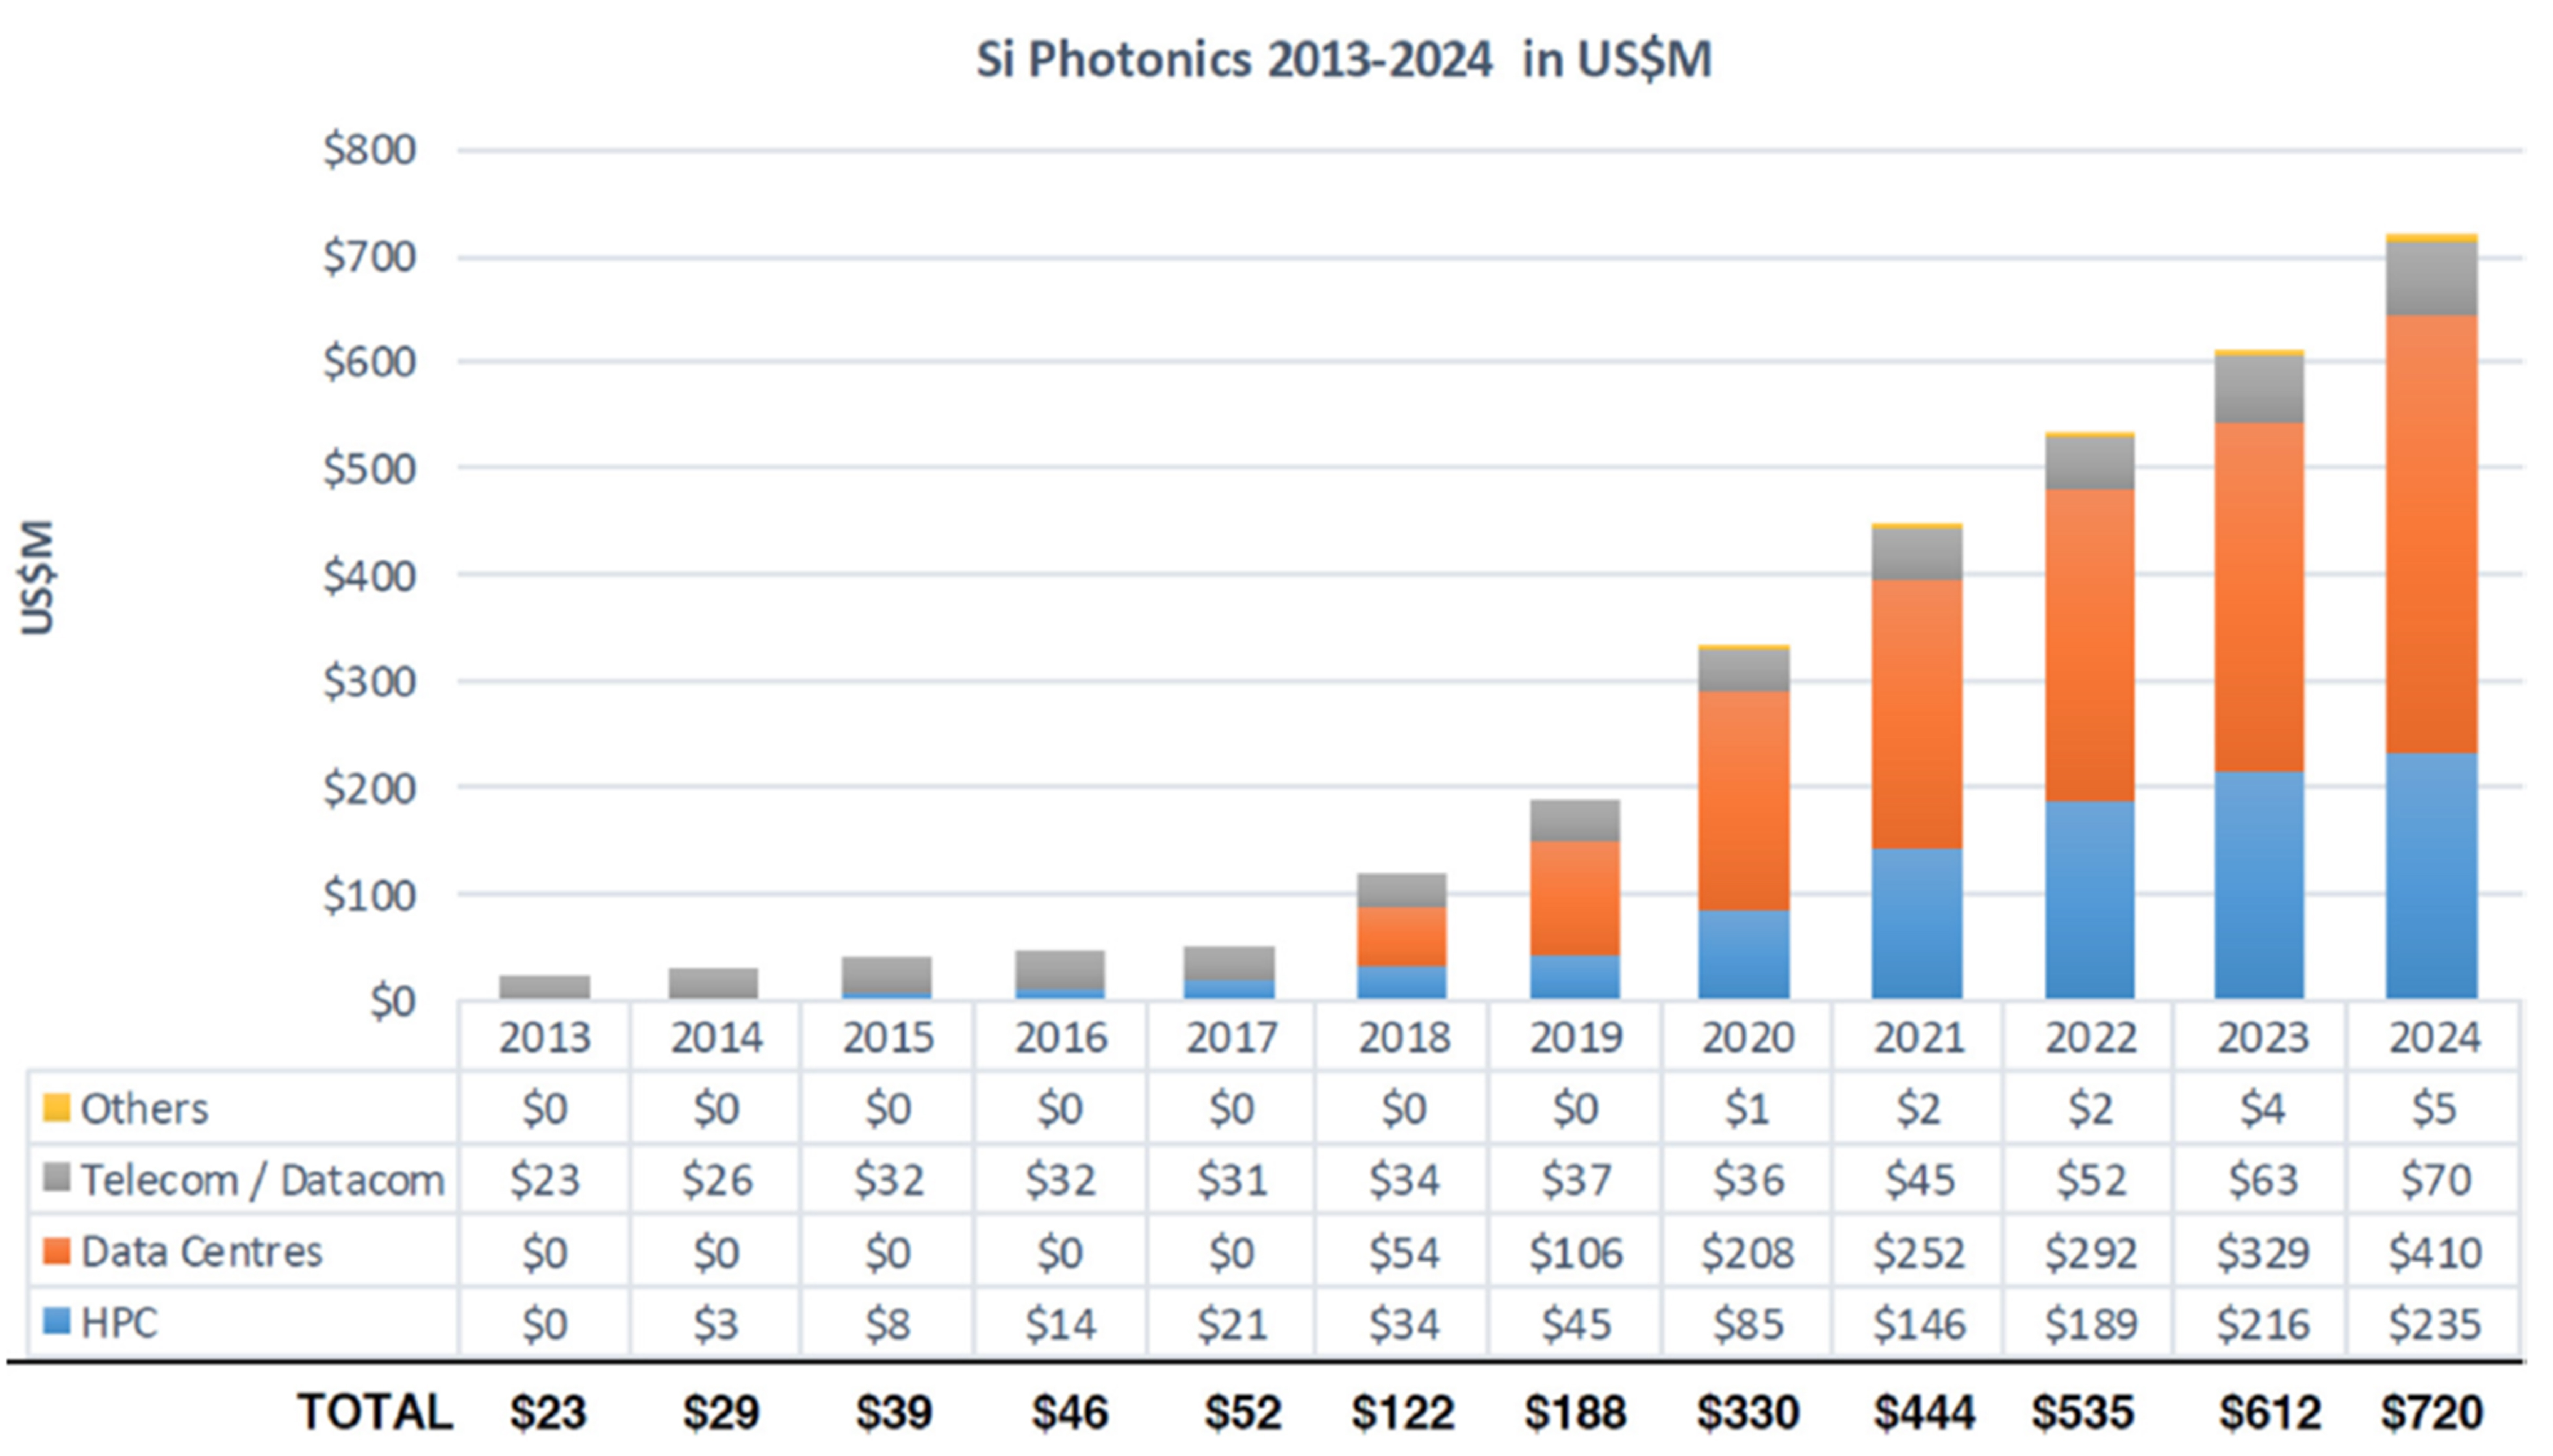
\includegraphics[width=0.8\textwidth]{../Pictures/intro_siliconphotonicsmarket.jpg}};
\begin{scope}[x={(image.south east)},y={(image.north west)}]
	%\draw[help lines,xstep=.1,ystep=.1] (0,0) grid (1,1); %参考线绘制
	\only<2>{\draw [ultra thick,line width=2mm,red,arrows=-{stealth},inner sep=4pt] (0.5,0.4) -- (0.9,0.9);}
\end{scope}
\end{tikzpicture}

\zihao{6}
市场咨询机构Yole Développement对2013年至2024年硅光芯片市场的预测
\end{frame}

\begin{frame}{硅基混合集成激光器}
\centering
\begin{tikzpicture}
\node[anchor=south west,inner sep=0] (image) at (0,0) {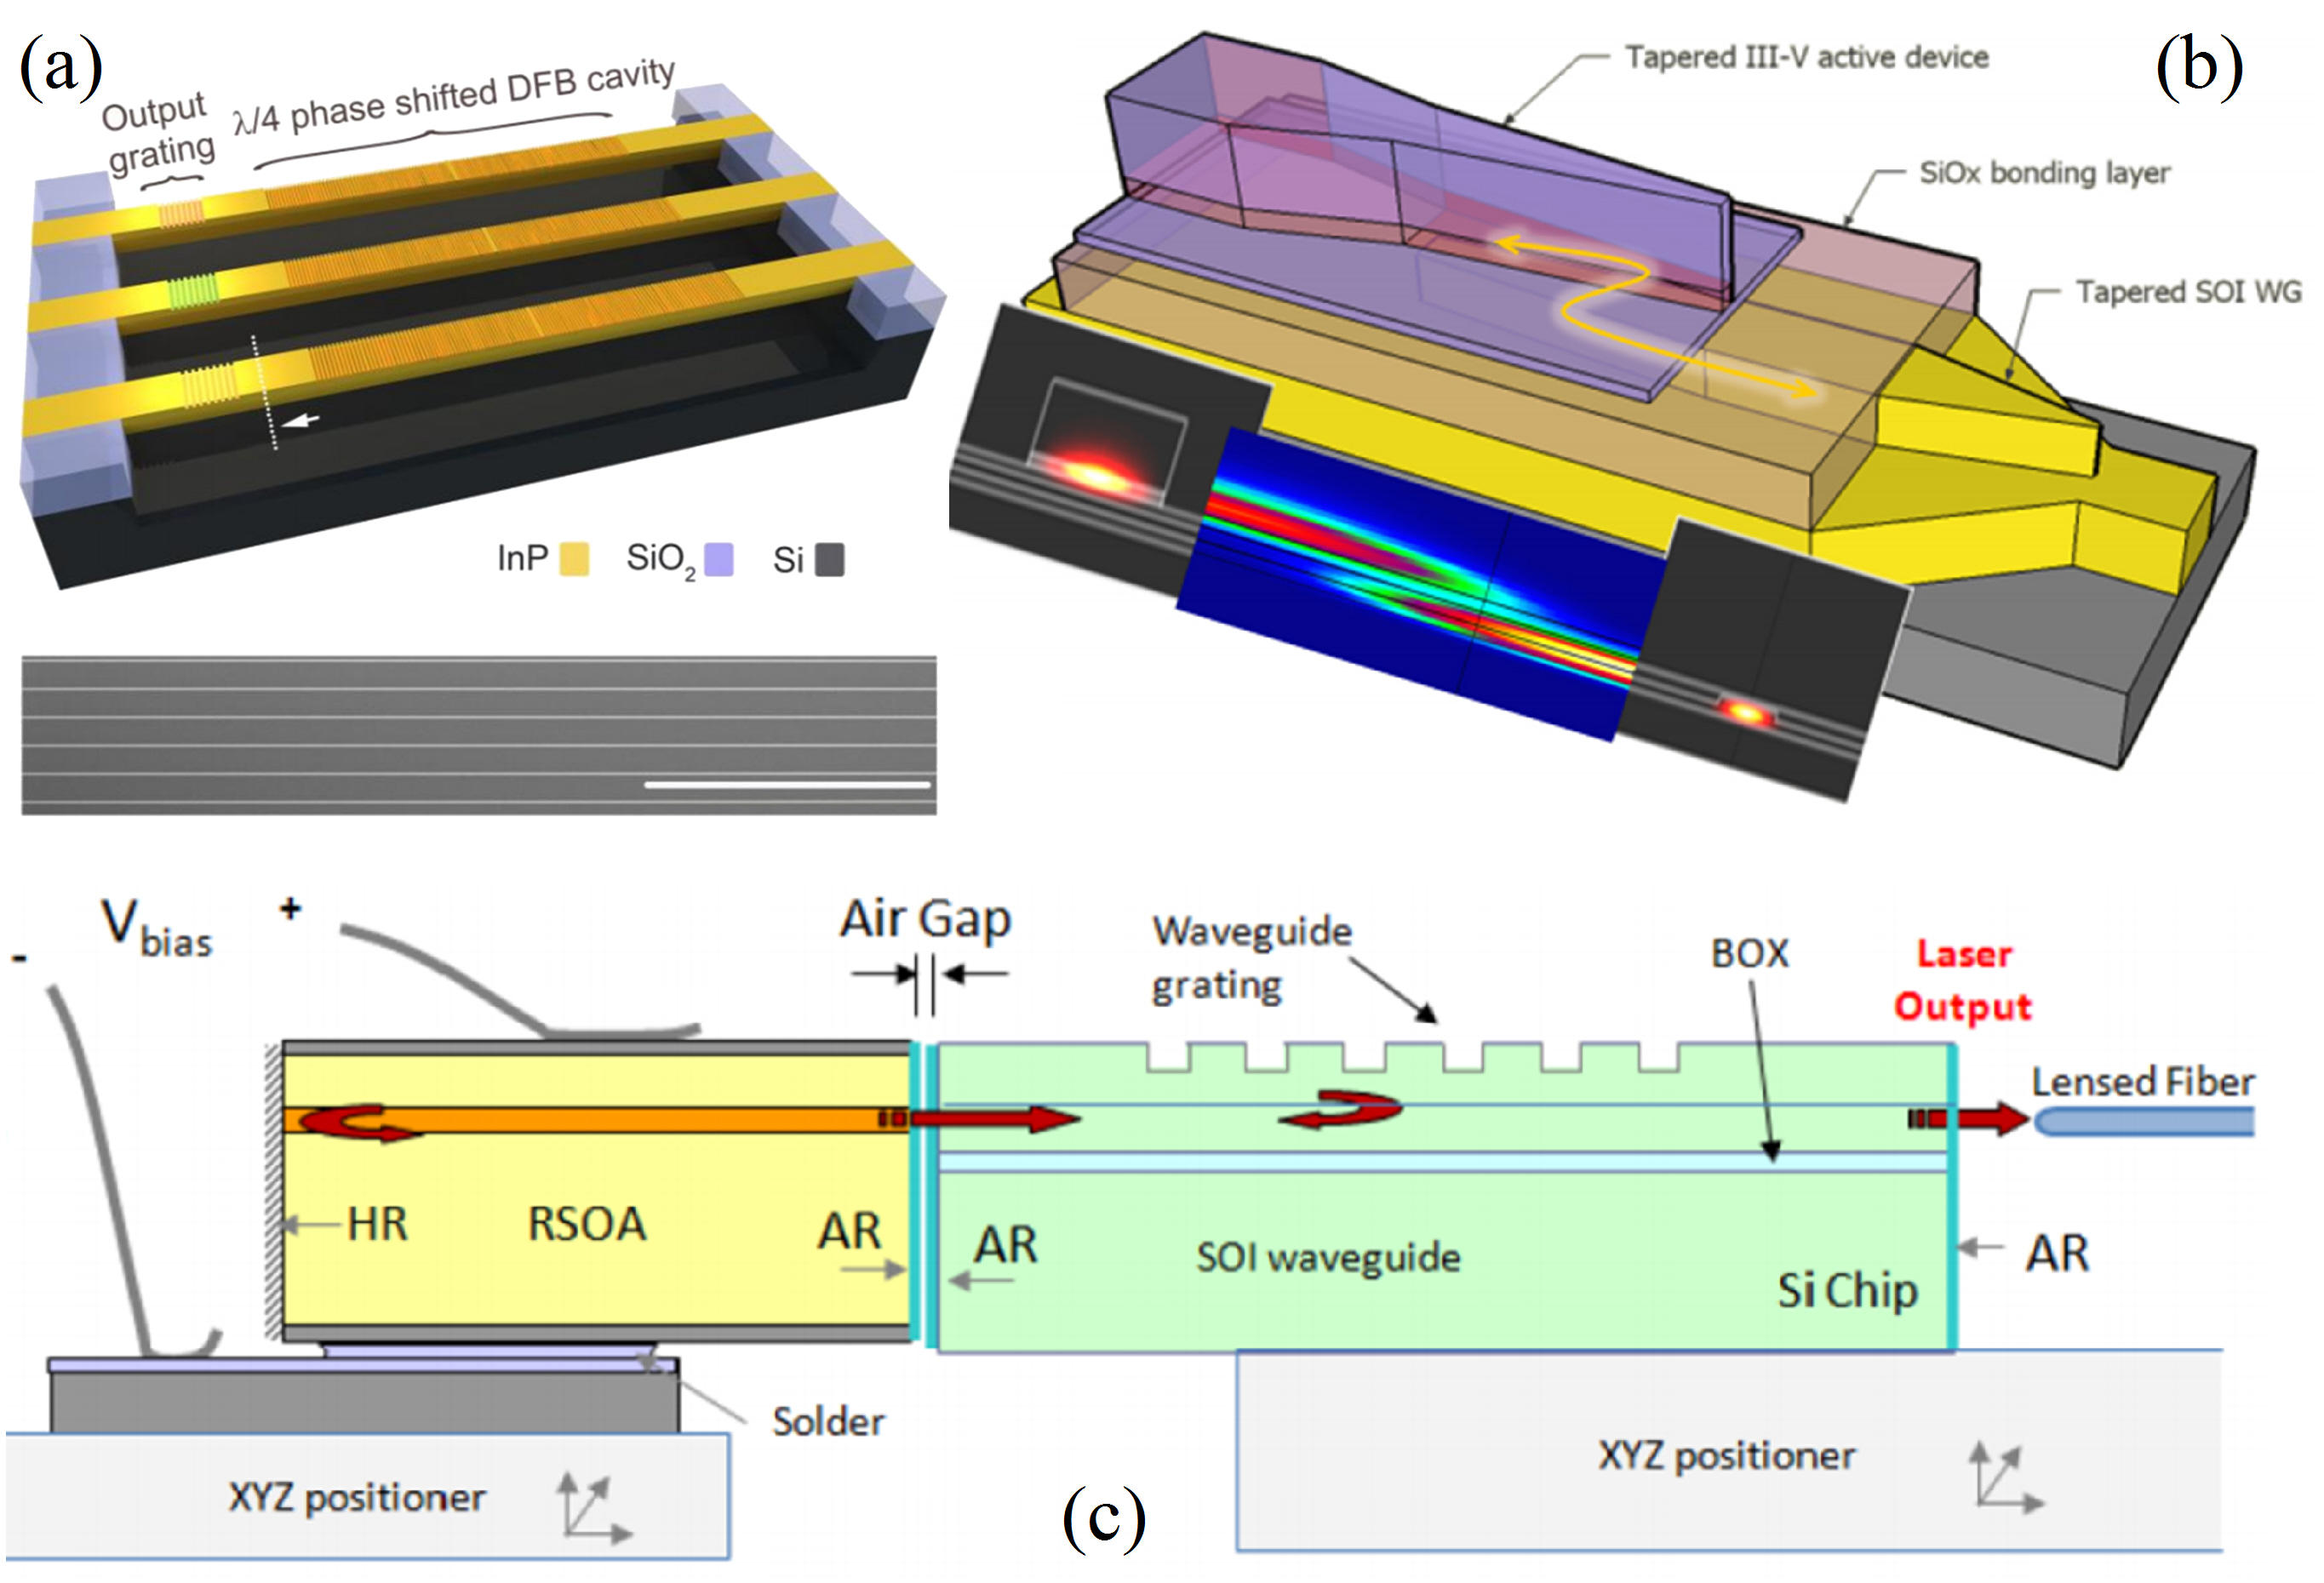
\includegraphics[width=0.9\textwidth]{../Pictures/intro_lasers.jpg}};
\begin{scope}[x={(image.south east)},y={(image.north west)}]
	%\draw[help lines,xstep=.1,ystep=.1] (0,0) grid (1,1); %参考线绘制
	\node[anchor = center,red,draw,font=\bfseries] at (0.2,0.62) {外延生长};
	\node[anchor = center,red,draw,font=\bfseries] at (0.85,0.62) {键合};
	\node[anchor = center,red,draw,font=\bfseries] at (0.47,0.1) {Flip-Chip};
	\node[anchor = north east,inner sep=0] at (0.4,0.48) {\bfseries\tiny \emph{Wang Z., Nature Photonics, 9(12)}};
	\node[anchor = north east,inner sep=0] at (0.97,0.48) {\bfseries\tiny \emph{Keyvaninia S., Opt. Exp., 21(3)}};
	\node[anchor = north east,inner sep=0] at (0.97,0.01) {\bfseries\tiny \emph{Zilkie A., Opt. Exp., 20(21)}};
\end{scope}
\end{tikzpicture}
\end{frame}

\begin{frame}{硅基\mbox{III-V}混合集成\mbox{DFB}激光器}
\begin{figure}
	\centering
	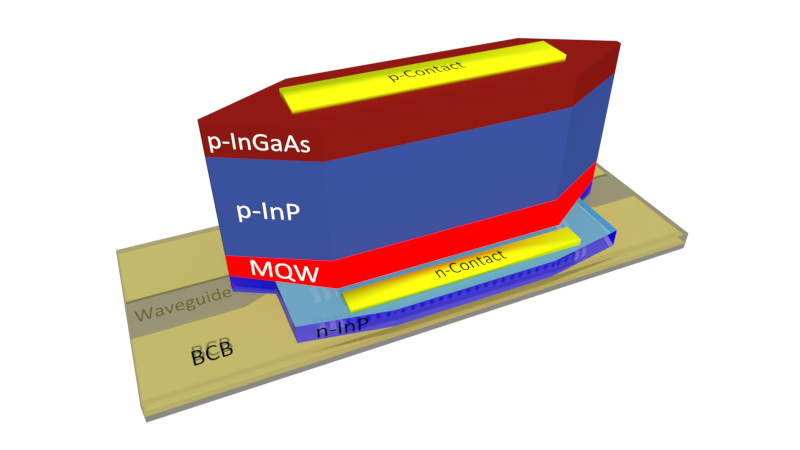
\includegraphics[width=\textwidth]{../Pictures/intro_heterogeneously_dfb_laser.png}
	%	\label{fig:blackhole}
\end{figure}
\end{frame}

\begin{frame}{\mbox{DFB}激光器的应用}
\centering
\begin{figure}
	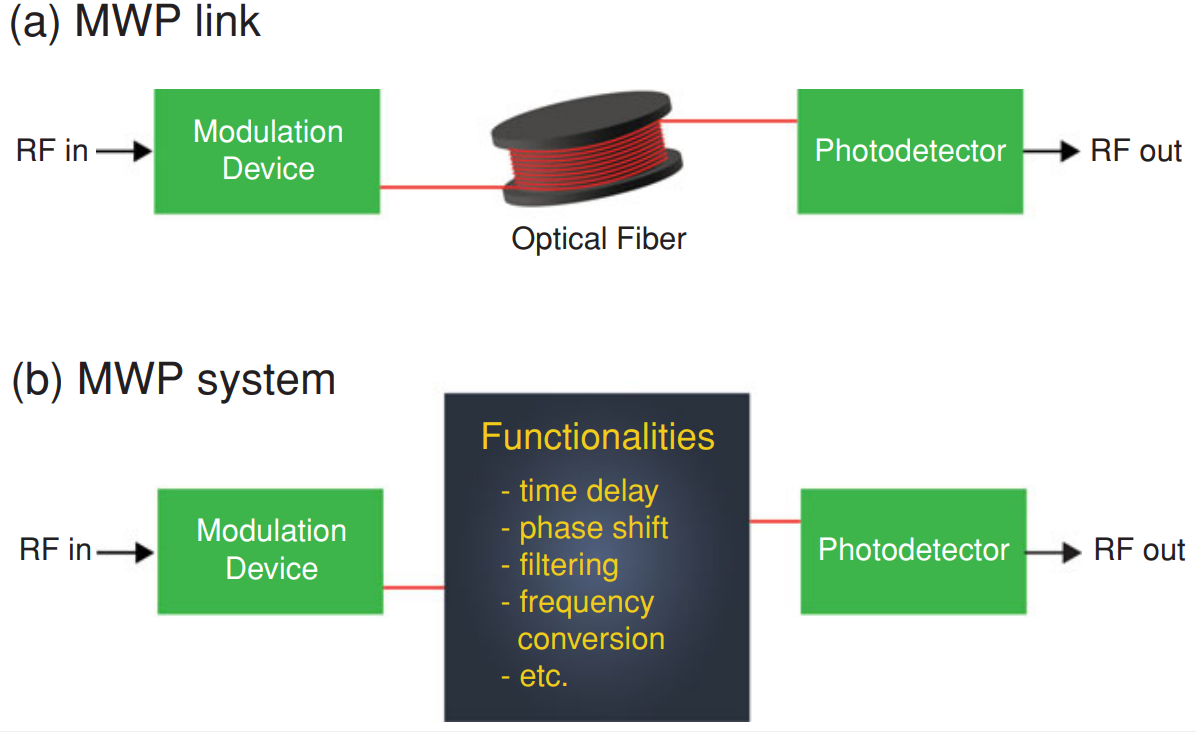
\includegraphics[width=0.8\textwidth]{../Pictures/intro_mwp.PNG}
	%	\label{fig:blackhole}
\end{figure}
\bfseries
微波光子学领域的应用
\end{frame}

\begin{frame}{\mbox{DFB}激光器的应用}
\centering
\begin{tikzpicture}
	\node[anchor=south west,inner sep=0] (image) at (0,0) {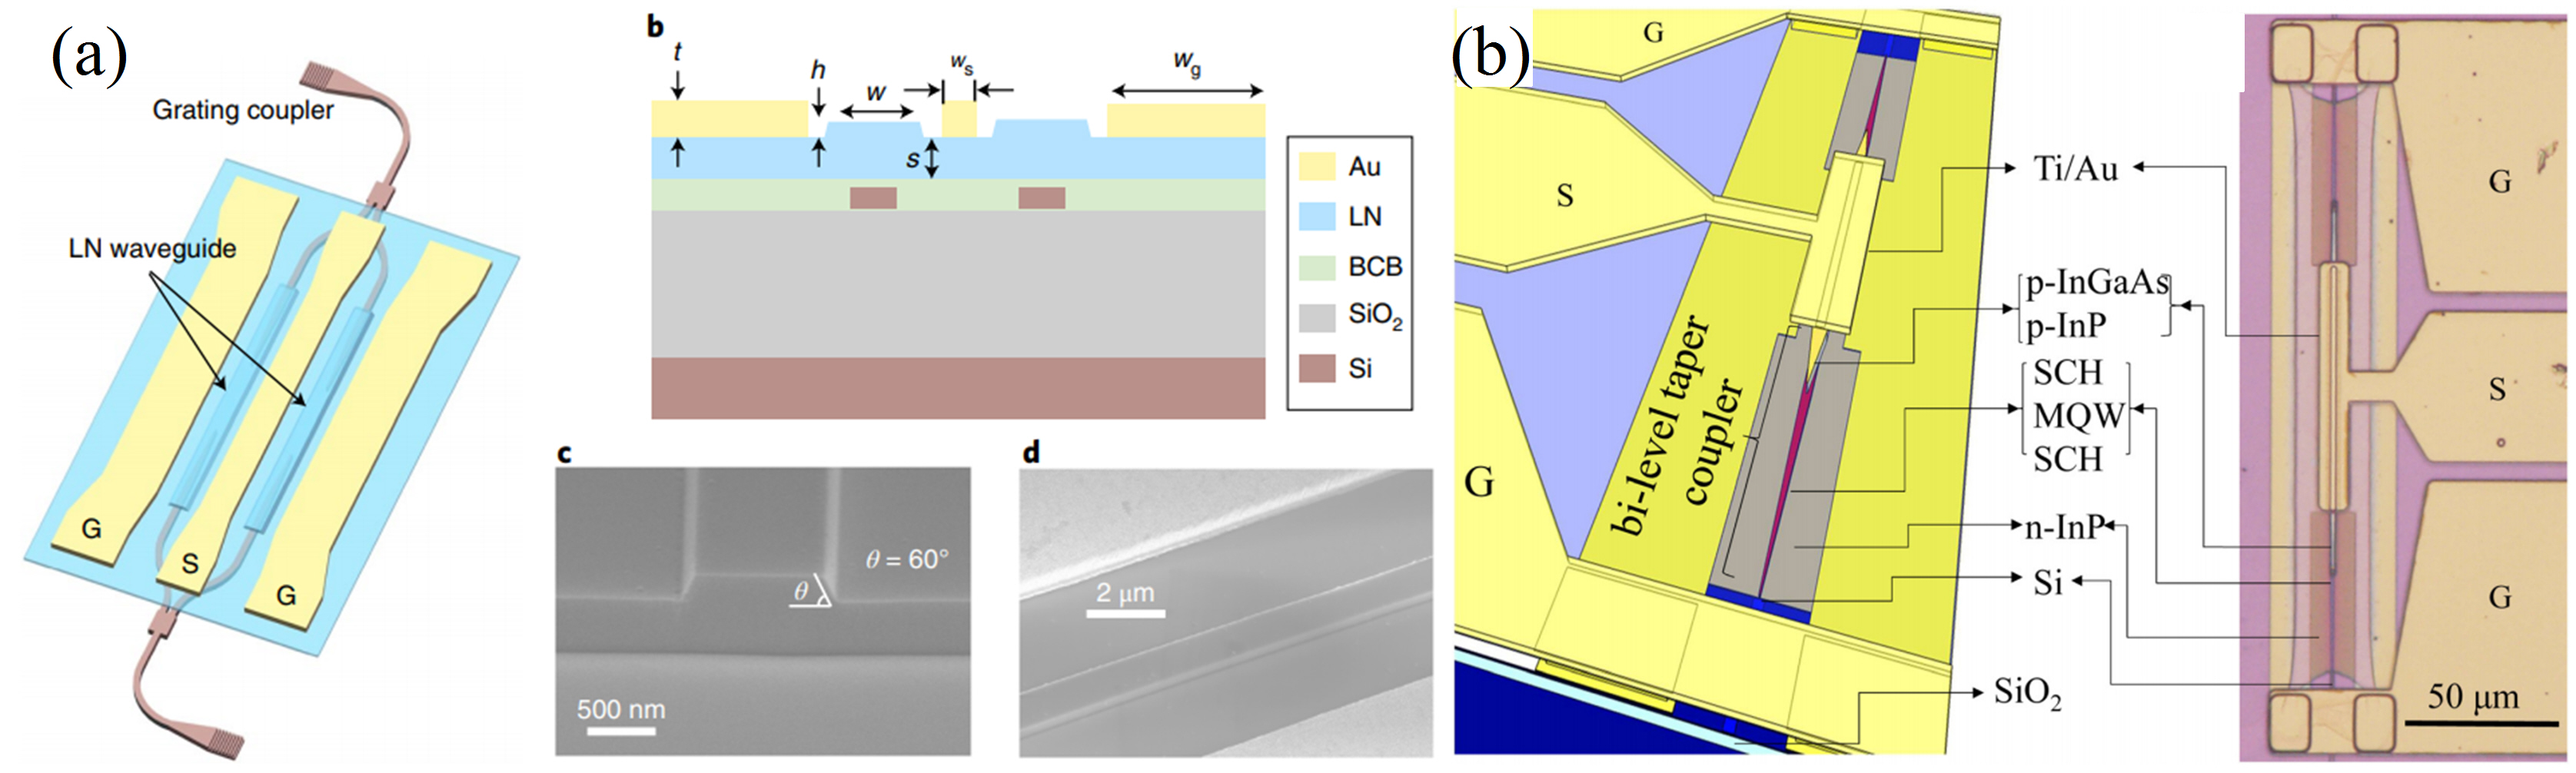
\includegraphics[width=\textwidth]{../Pictures/intro_external_modulator.jpg}};
	\begin{scope}[x={(image.south east)},y={(image.north west)}]
		%\draw[help lines,xstep=.1,ystep=.1] (0,0) grid (1,1); %参考线绘制
		\node[anchor = north east,inner sep=0] at (0.56,0) {\bfseries\tiny \emph{He M., Nature Photonics, 2019:1}};
		\node[anchor = north east,inner sep=0] at (1,0) {\bfseries\tiny \emph{Huang Q., Applied Physics Lett., 108(14)}};
	\end{scope}
\end{tikzpicture}
\\\vspace{0.5cm}
\bfseries
光互联领域的应用
\end{frame}

\begin{frame}{\mbox{DFB}激光器的应用}
\centering
\begin{figure}
	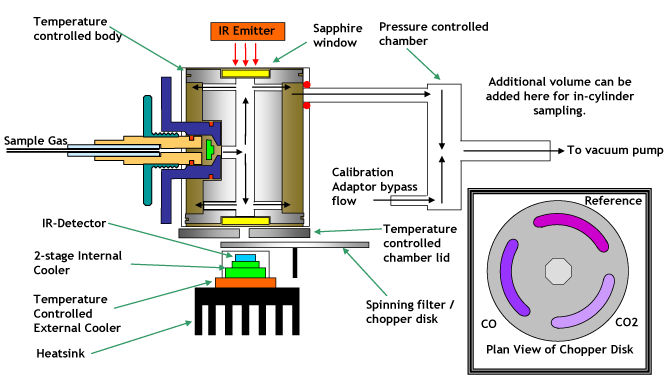
\includegraphics[width=0.9\textwidth]{../Pictures/intro_ndir.PNG}
	%	\label{fig:blackhole}
\end{figure}
\bfseries
气体检测领域的应用
\end{frame}

\section{研究内容}
\subsection{\mbox{SOI}刻蚀中的显色特性研究}
\frame{\tableofcontents[currentsubsection]}
%\subsubsection{光学微波信号的产生与锁定}
%\subsubsection{\mbox{DFB}激光器调制带宽的提升}

\begin{frame}{背景介绍}
\centering
\begin{tikzpicture}
	\only<1>{\node[anchor=south west,inner sep=0] (image) at (0,0) {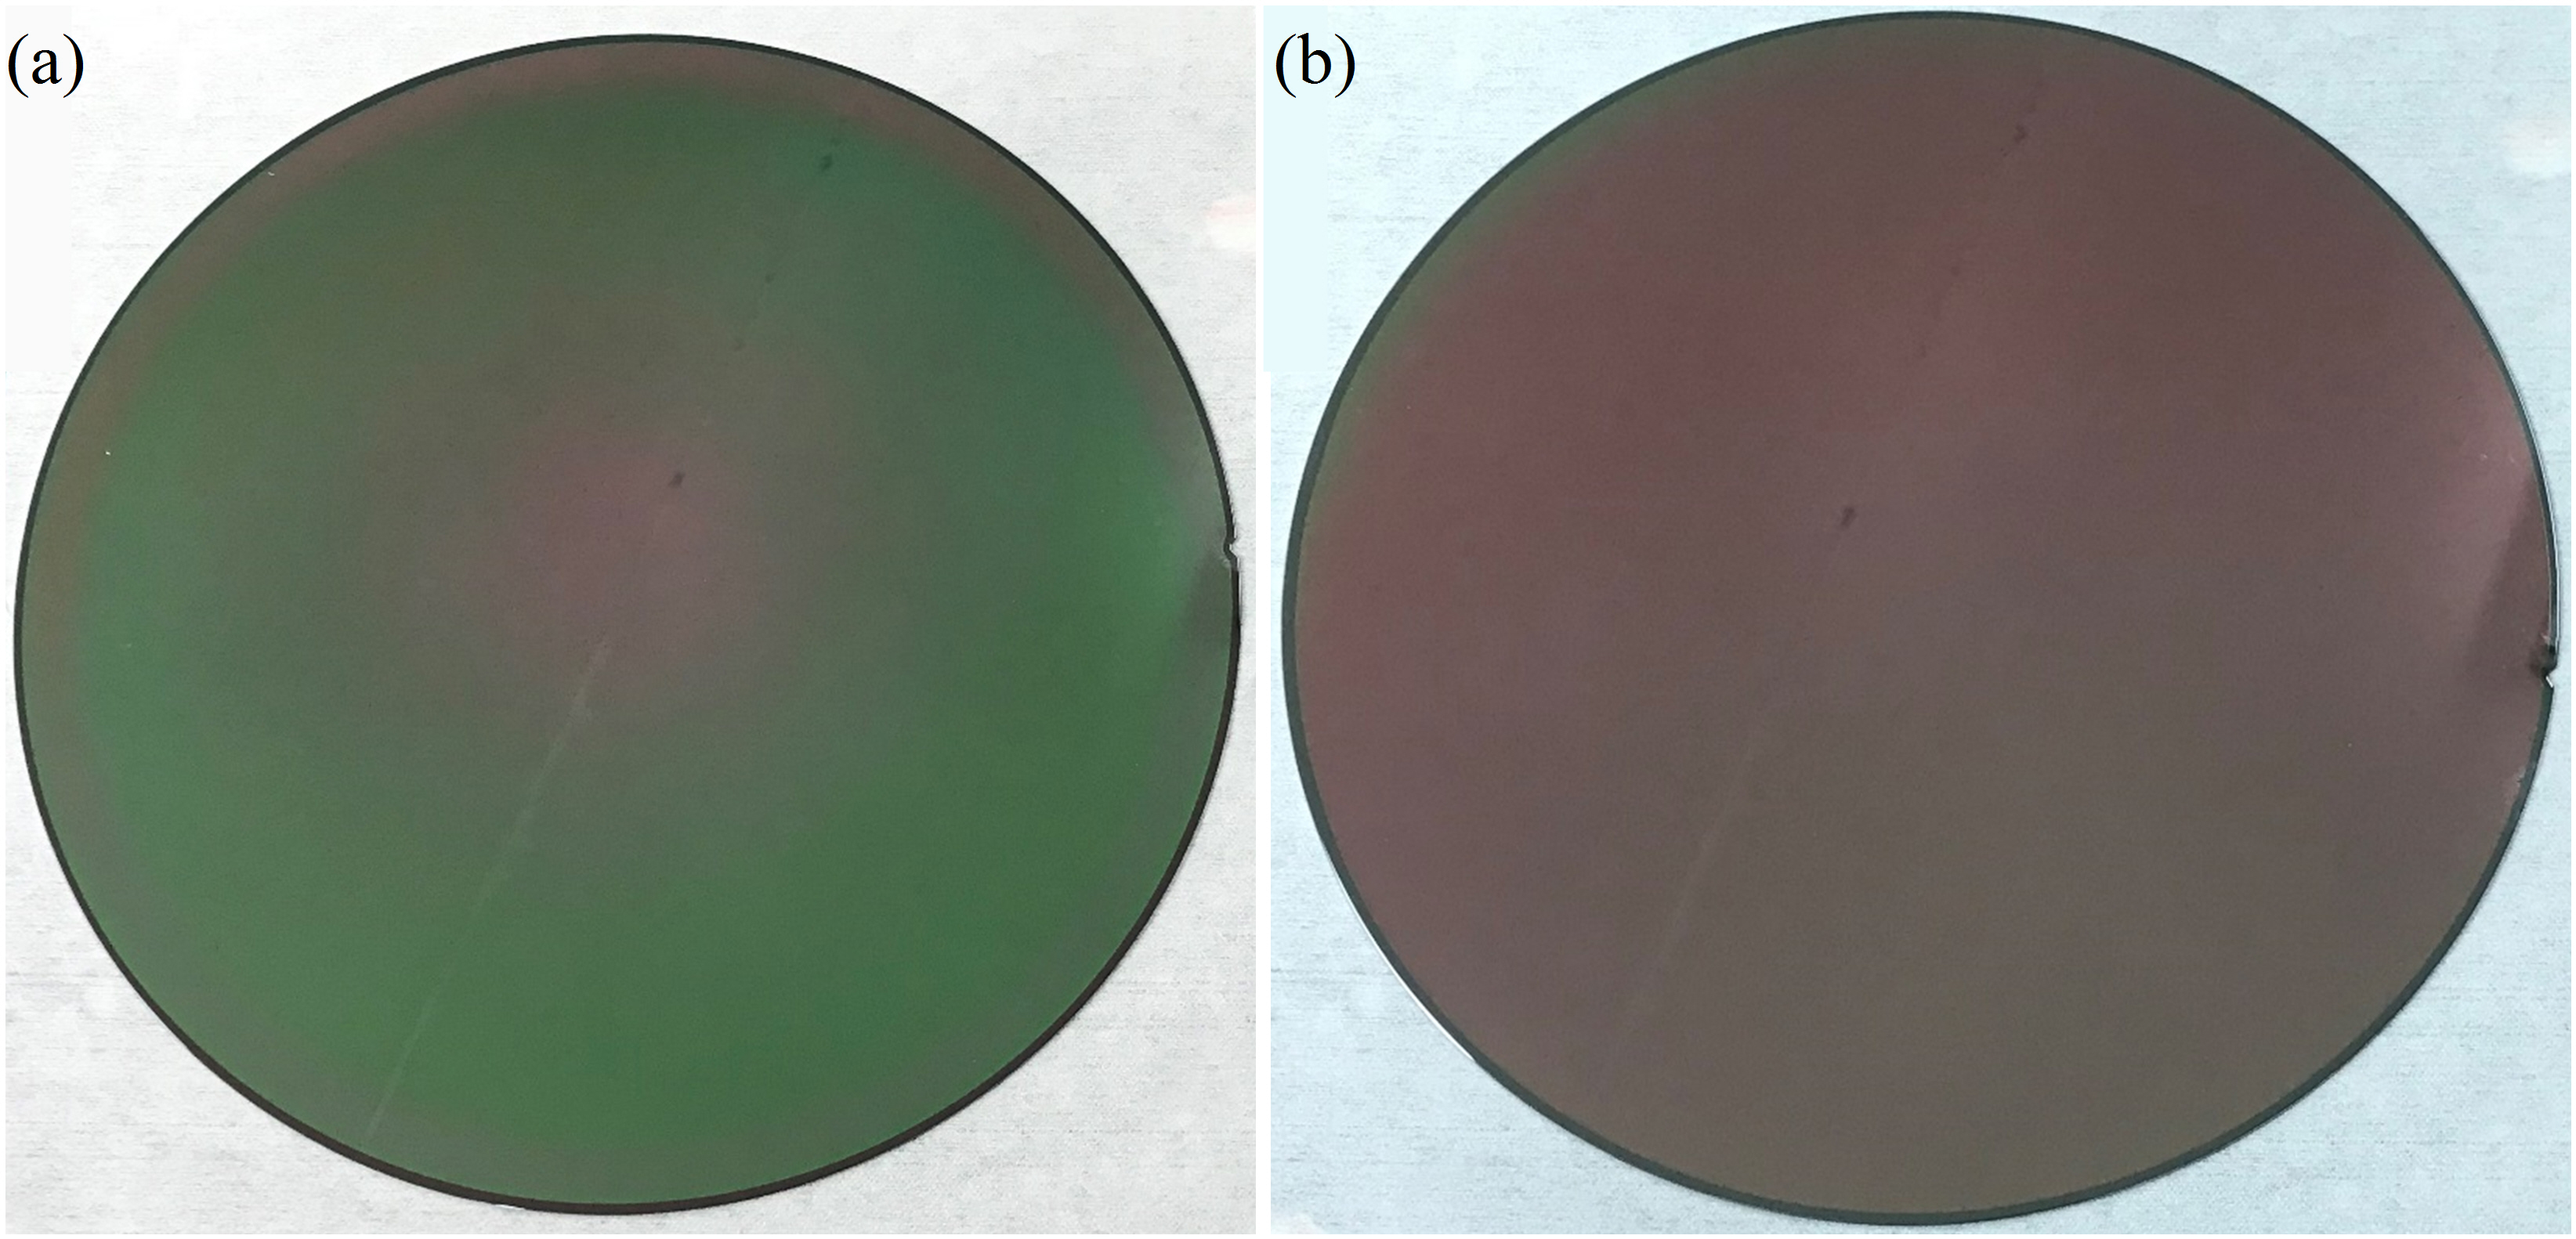
\includegraphics[width=0.9\textwidth]{../Pictures/color_wafer.jpg}};	
		\begin{scope}[x={(image.south east)},y={(image.north west)}]
		\node at (0.25,-0.05) {220$nm$~SOI};
		\node at (0.75,-0.05) {340$nm$~SOI};
		\node[anchor = north,font=\bfseries] at (0.5,-0.15) {\mbox{SOI}不同硅层厚度显示不同颜色};
		\end{scope}}
	\only<2>{\node[anchor=south west,inner sep=0] (image) at (0,0) {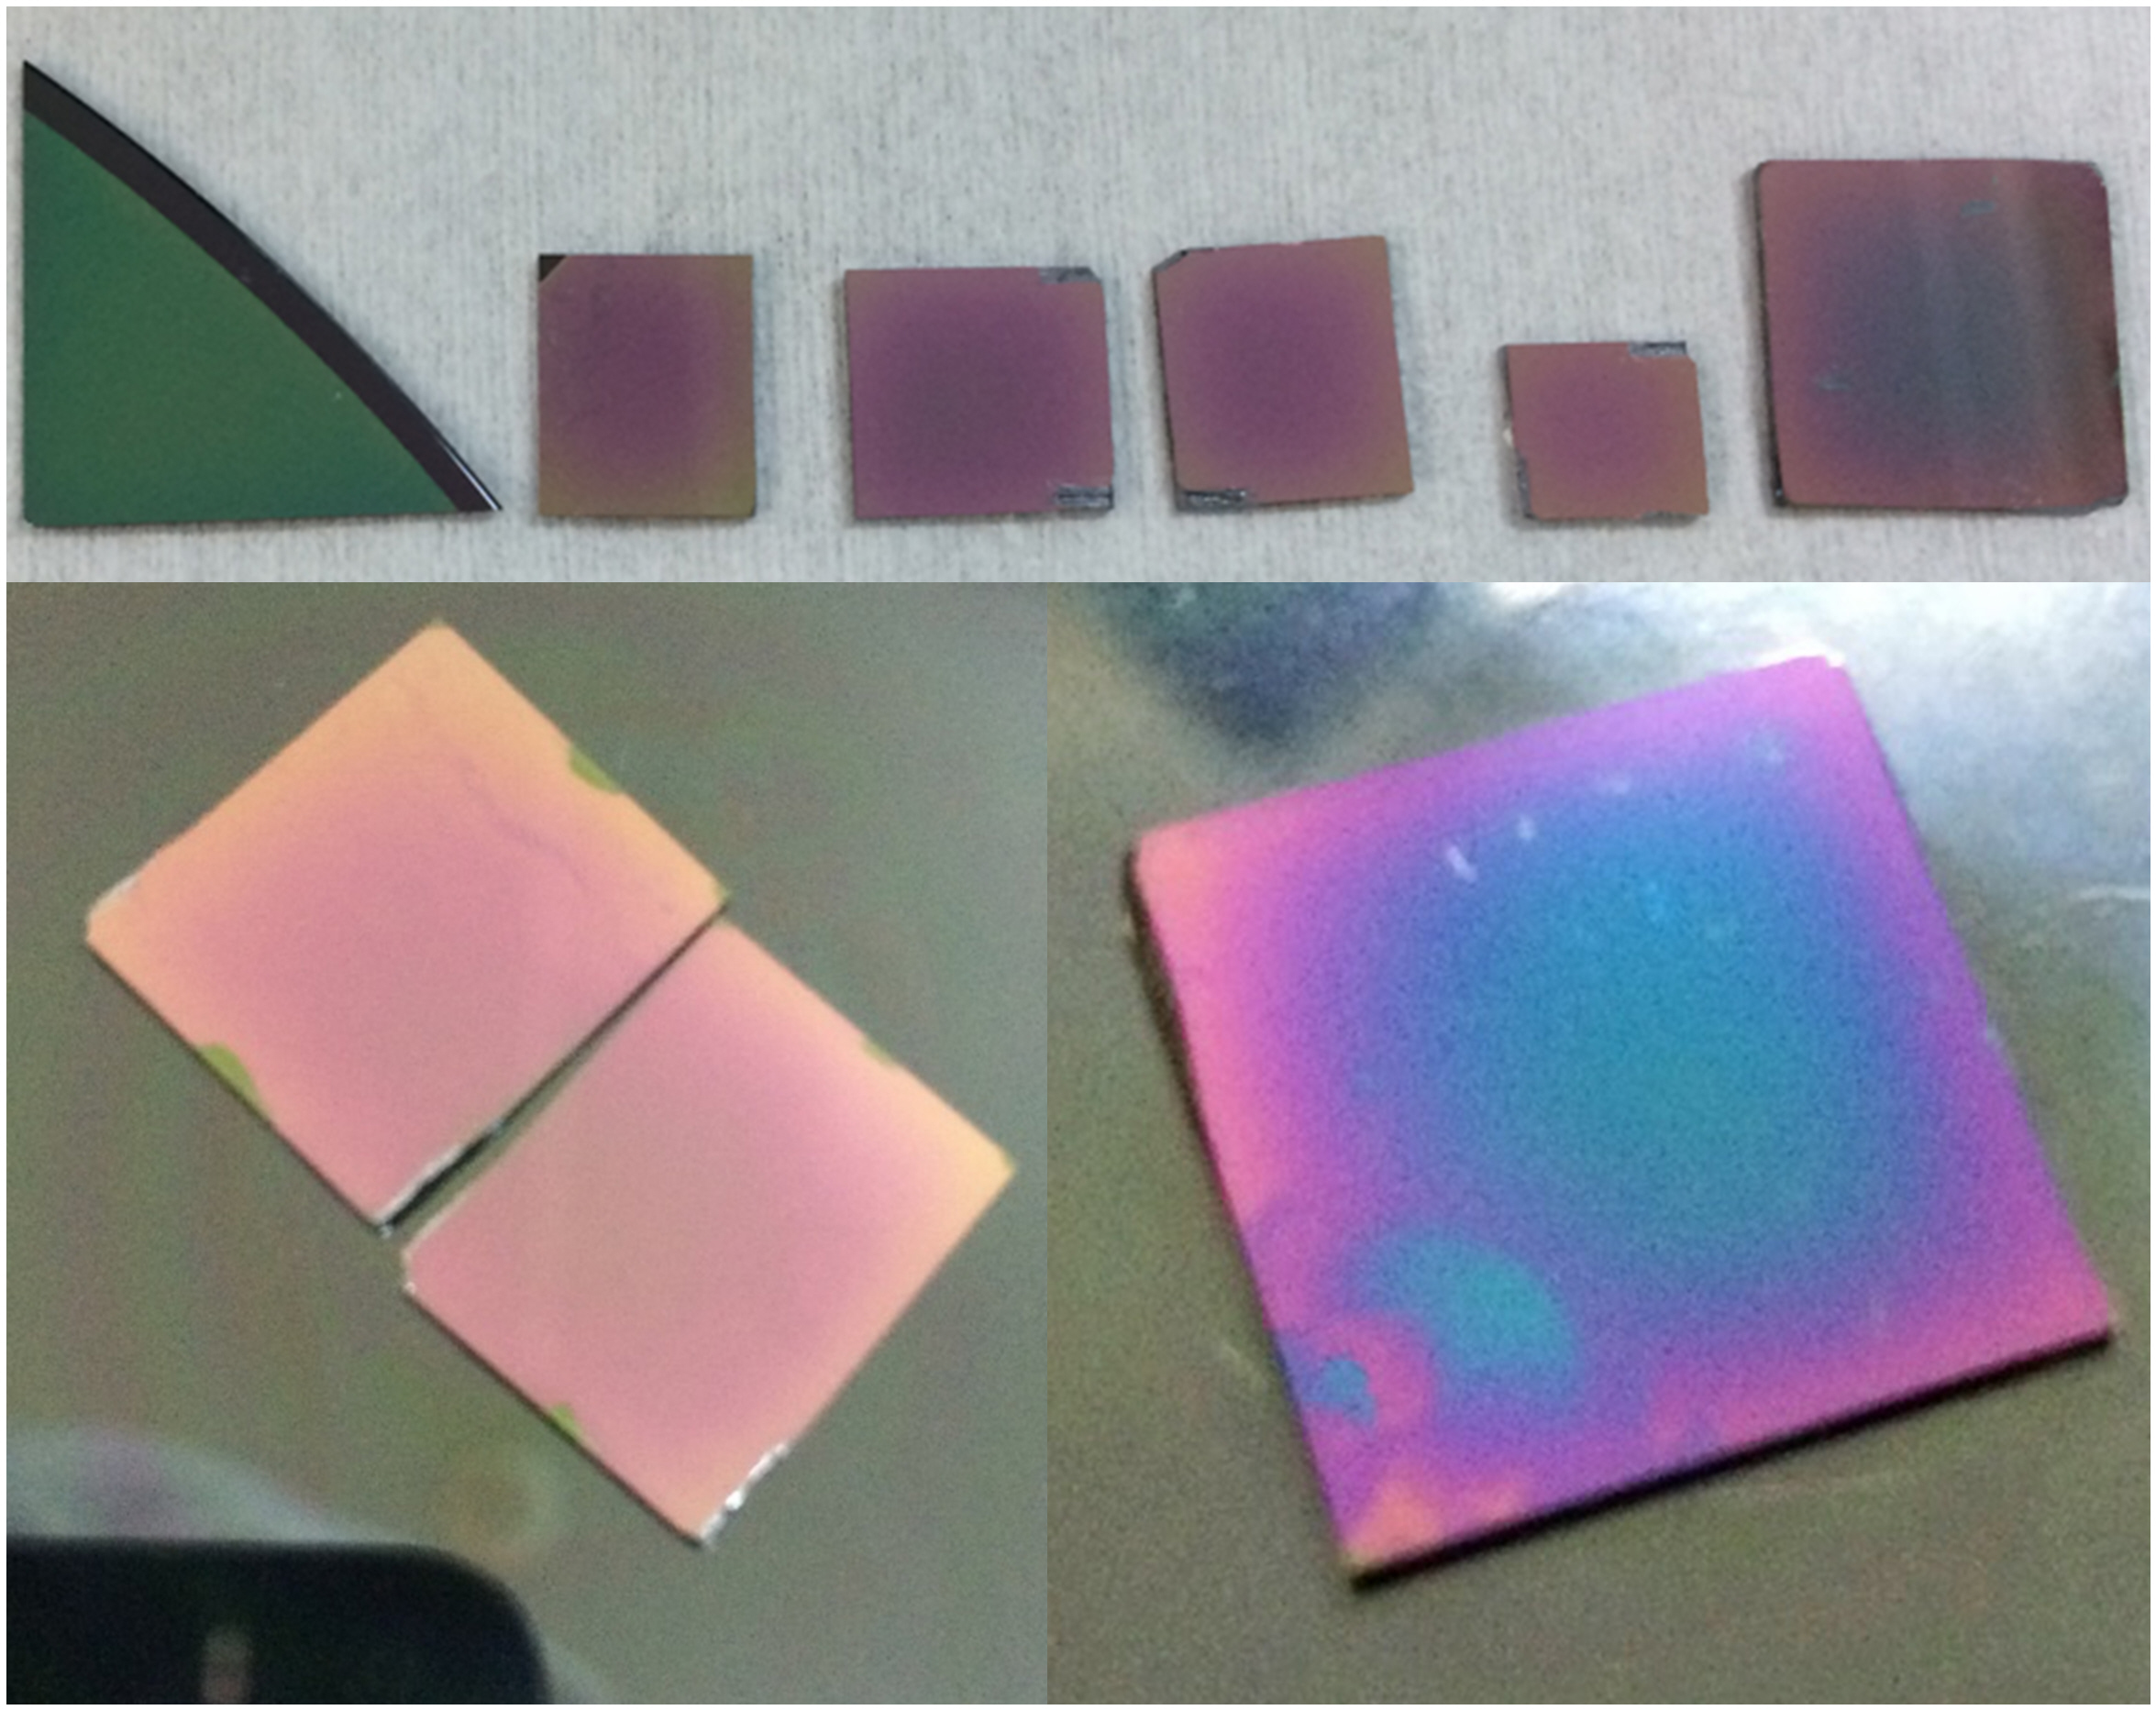
\includegraphics[width=0.7\textwidth]{../Pictures/color_etch_time.jpg}};	
		\begin{scope}[x={(image.south east)},y={(image.north west)}]
		\node at (0.5,-0.05) {不同刻蚀深度对应的\mbox{SOI}的颜色};
		\node[anchor = north,red,draw,font=\bfseries] at (0.73,0.2) {\mbox{ICP}刻蚀速率不均匀};
		\end{scope}}
	\only<3>{\node[anchor=south west,inner sep=0] (image) at (0,0) {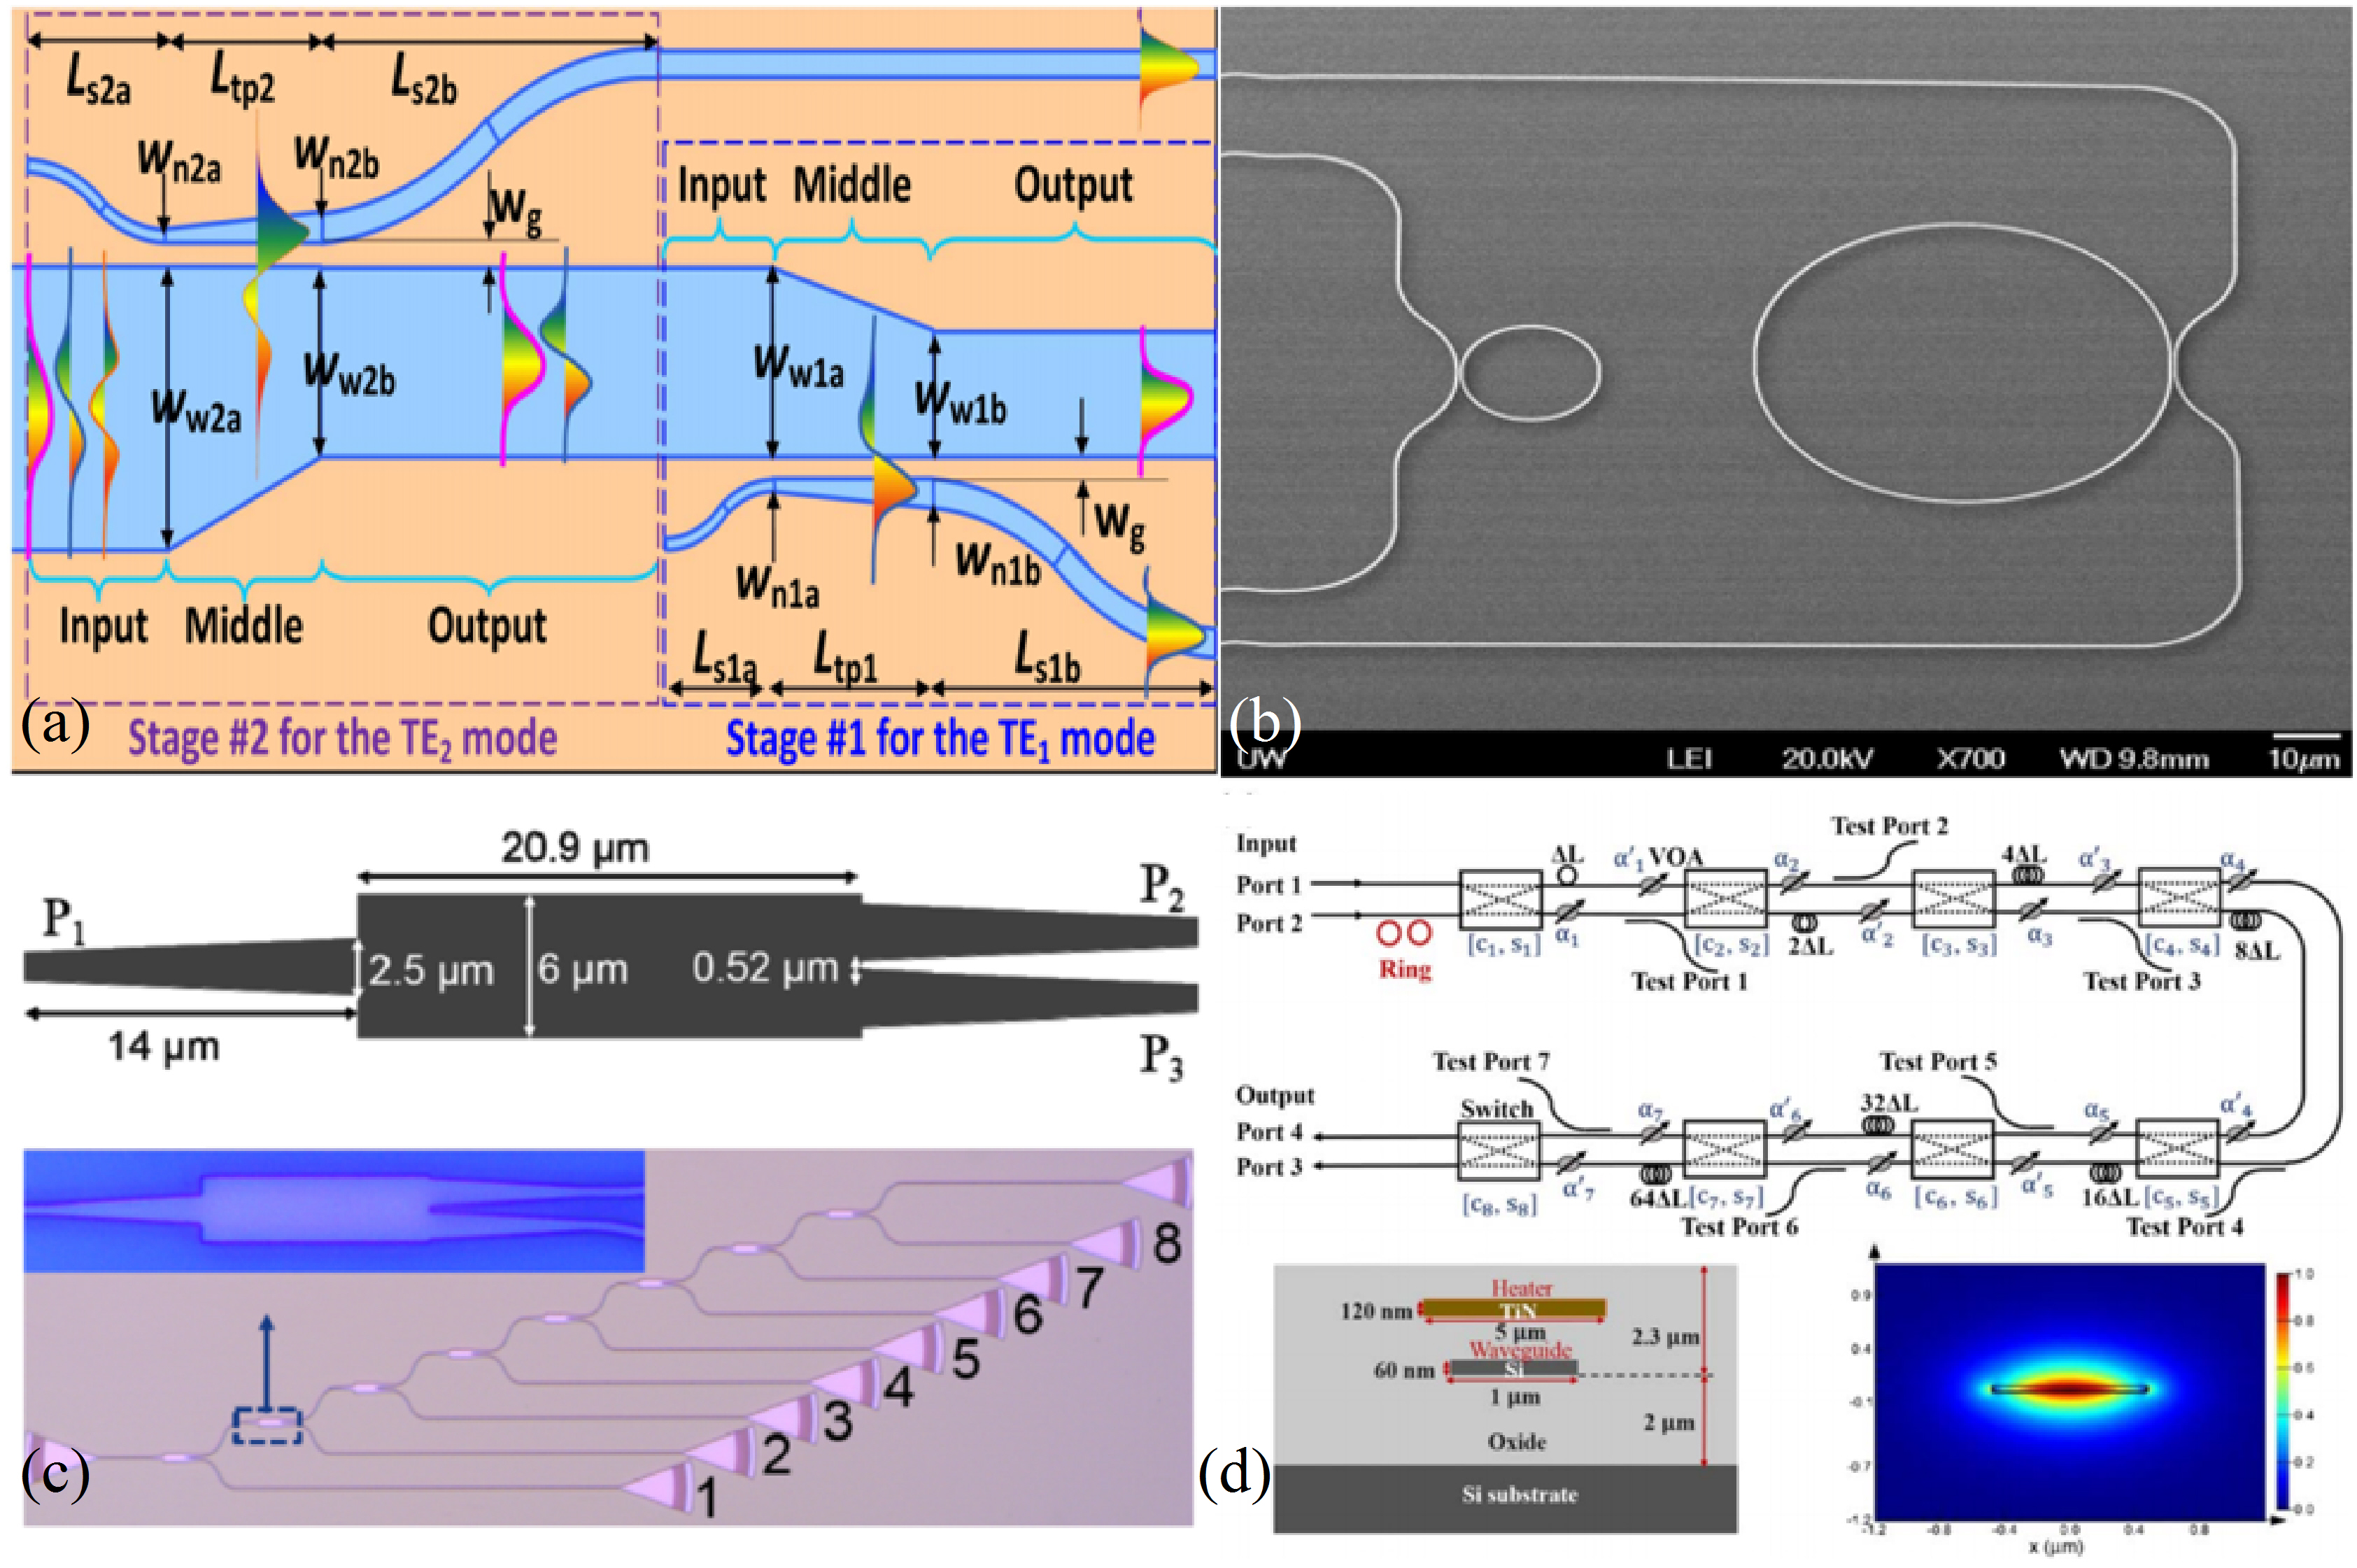
\includegraphics[width=0.9\textwidth]{../Pictures/color_thin_application.jpg}};	
		\begin{scope}[x={(image.south east)},y={(image.north west)}]
		%\draw[help lines,xstep=.1,ystep=.1] (0,0) grid (1,1); %参考线绘制
		\node at (0.5,-0.05) {超薄硅器件};
		\node[anchor = north,red,draw,font=\bfseries] at (0.25,0.7) {模分复用解复用器:50$nm$};
		\node[anchor = north,red,draw,font=\bfseries] at (0.75,0.7) {微环传感器:90$nm$};
		\node[anchor = north,red,draw,font=\bfseries] at (0.25,0.35) {多模干涉耦合器:$60nm$};
		\node[anchor = north,red,draw,font=\bfseries] at (0.75,0.35) {延时线:60$nm$};
		\node[anchor = north east] at (0.52,0.52) {\bfseries\tiny \emph{Li C., Opt. Lett., 42(12)}};
		\node[anchor = north east] at (1.01,0.52) {\bfseries\tiny \emph{Fard S., Opt. Exp., 22(12)}};
		\node[anchor = south east] at (0.52,-0.02-5pt) {\bfseries\tiny \emph{Zou Z., Opt. Exp., 23(16)}};
		\node[anchor = south east] at (1.01,-0.02-5pt) {\bfseries\tiny \emph{Wang X., Optica, 4(5)}};
		\end{scope}}
\end{tikzpicture}
\end{frame}

\begin{frame}{背景介绍}
\centering
\begin{tikzpicture}
\node[anchor=south west,inner sep=0] (image) at (0,0) {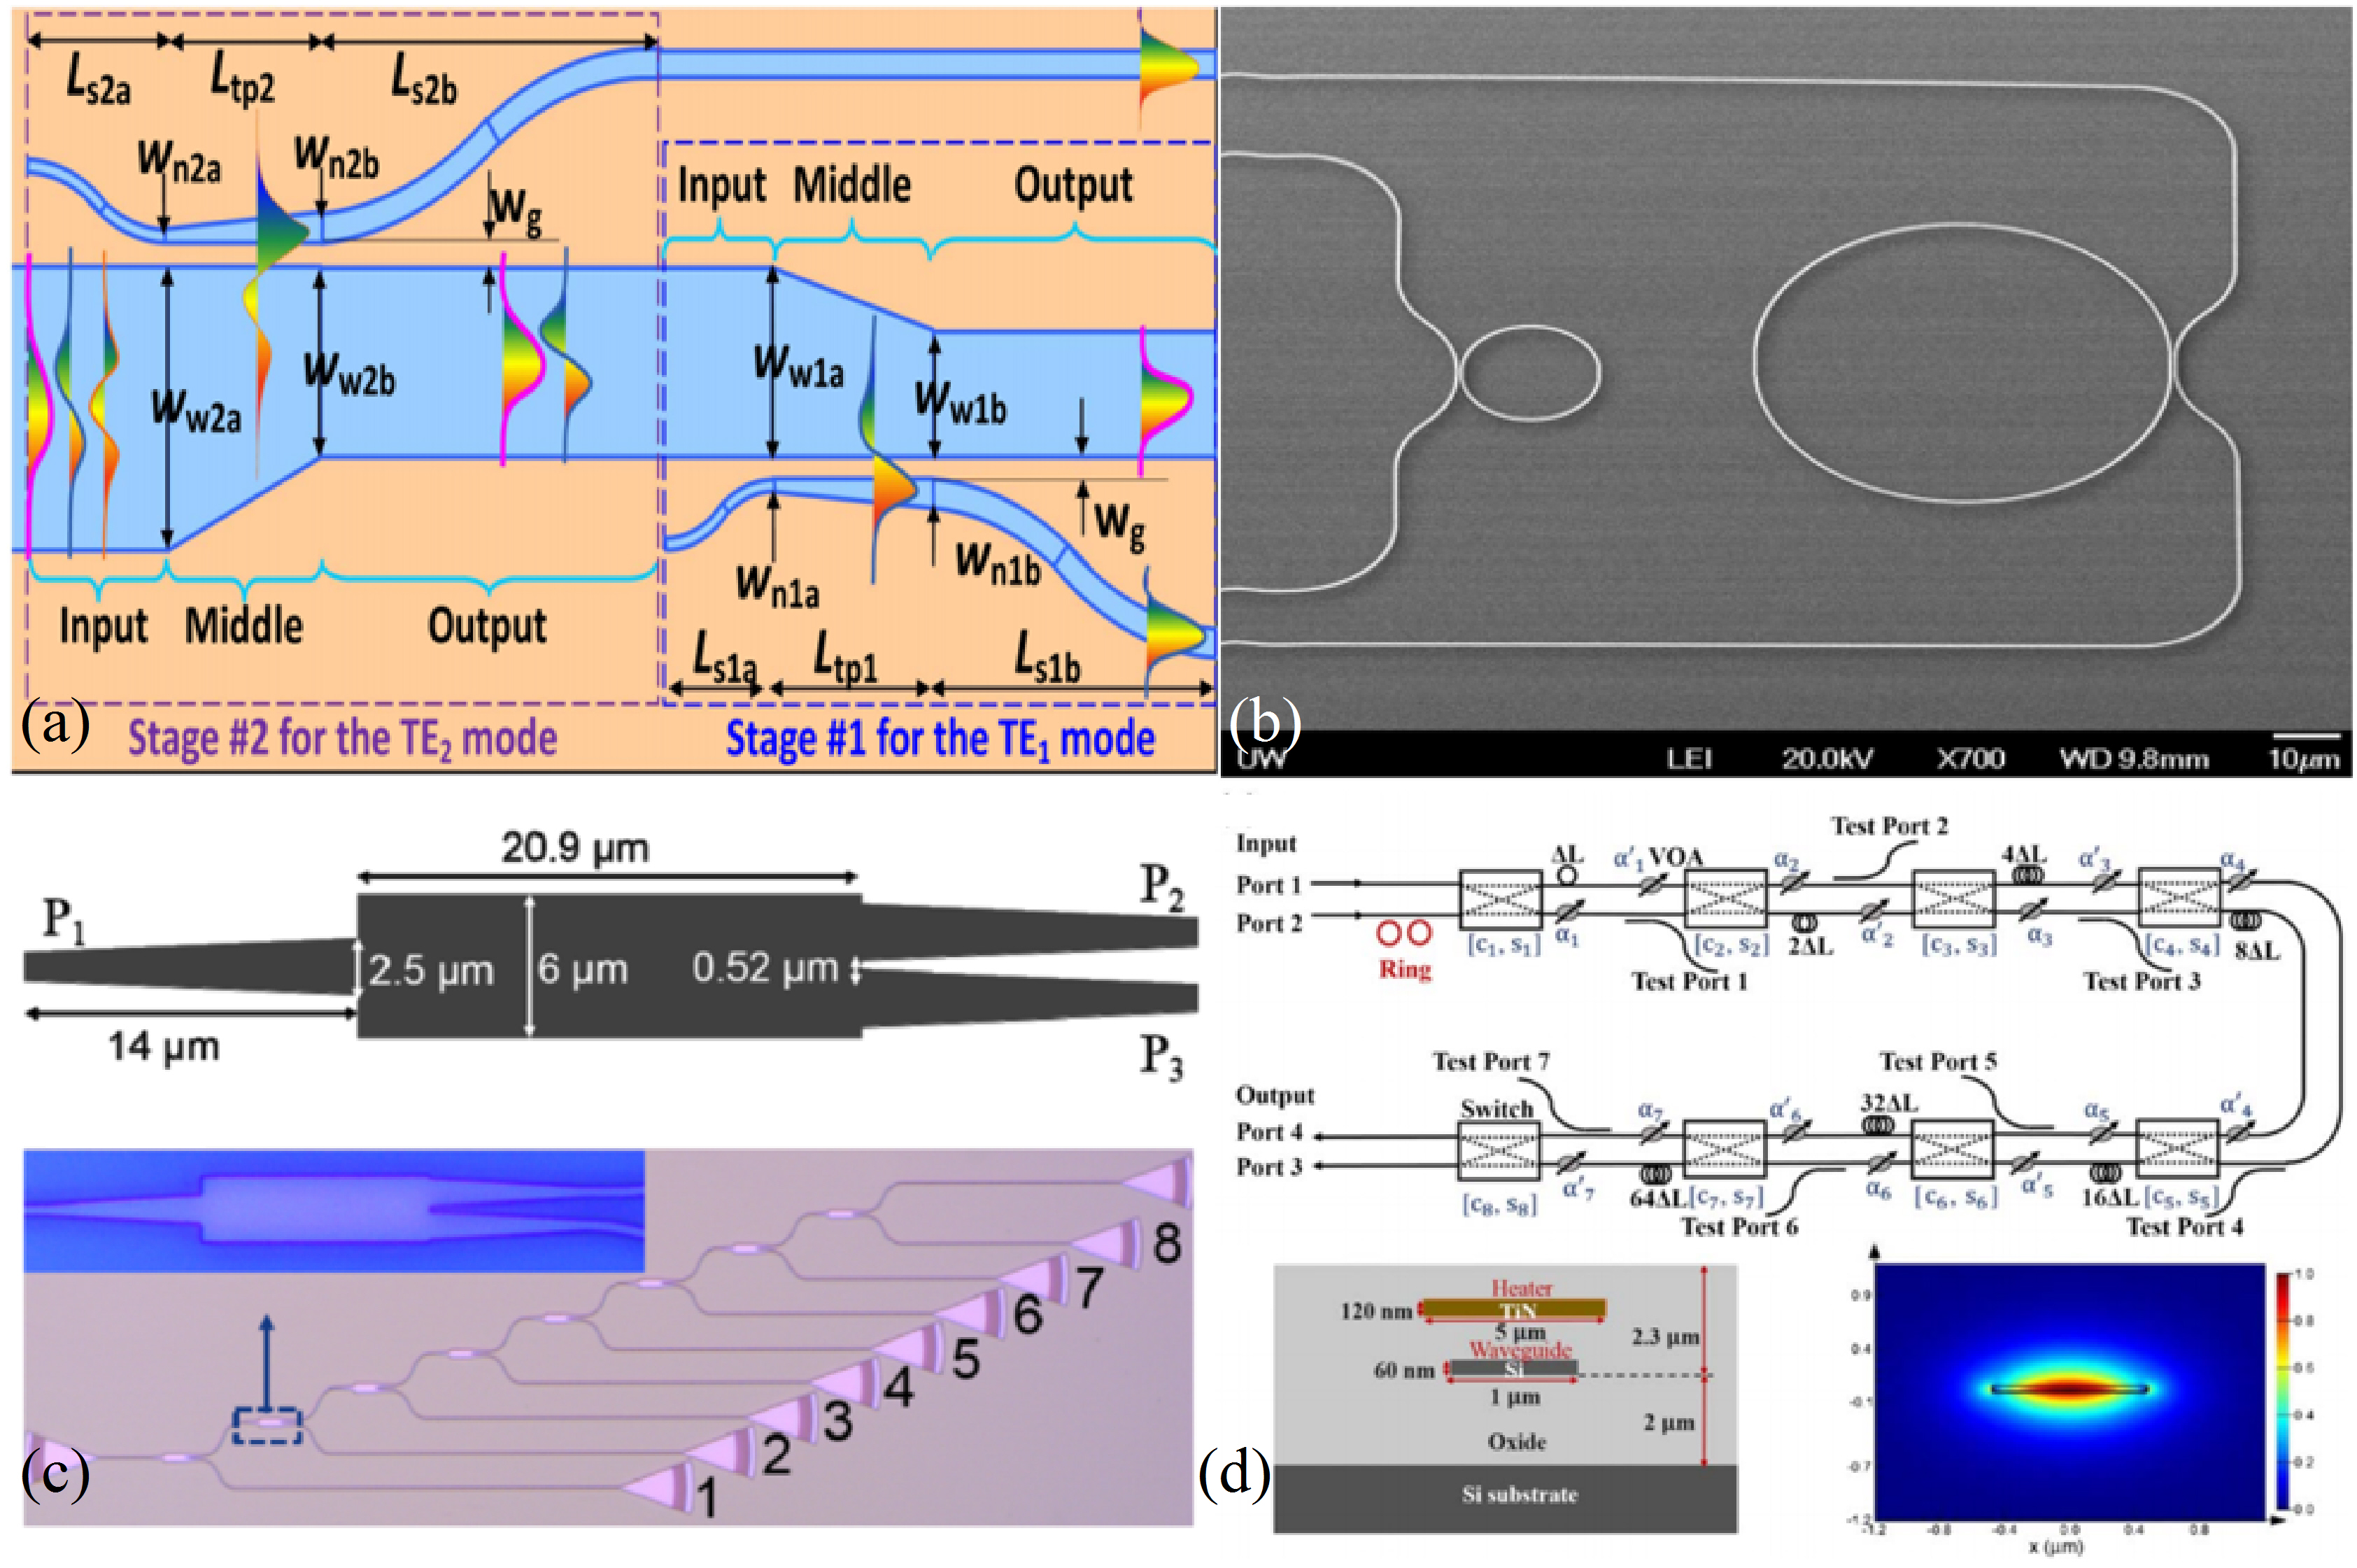
\includegraphics[width=0.9\textwidth]{../Pictures/color_thin_application}};
\begin{scope}[x={(image.south east)},y={(image.north west)}]
	%\draw[help lines,xstep=.1,ystep=.1] (0,0) grid (1,1); %参考线绘制
	\fill [draw=none, fill=white, fill opacity=0.7] (image.north west) -- (image.north east) -- (image.south east) -- (image.south west) -- (image.north west) -- cycle;
	\node[anchor = center,inner sep=0] at (image.center) {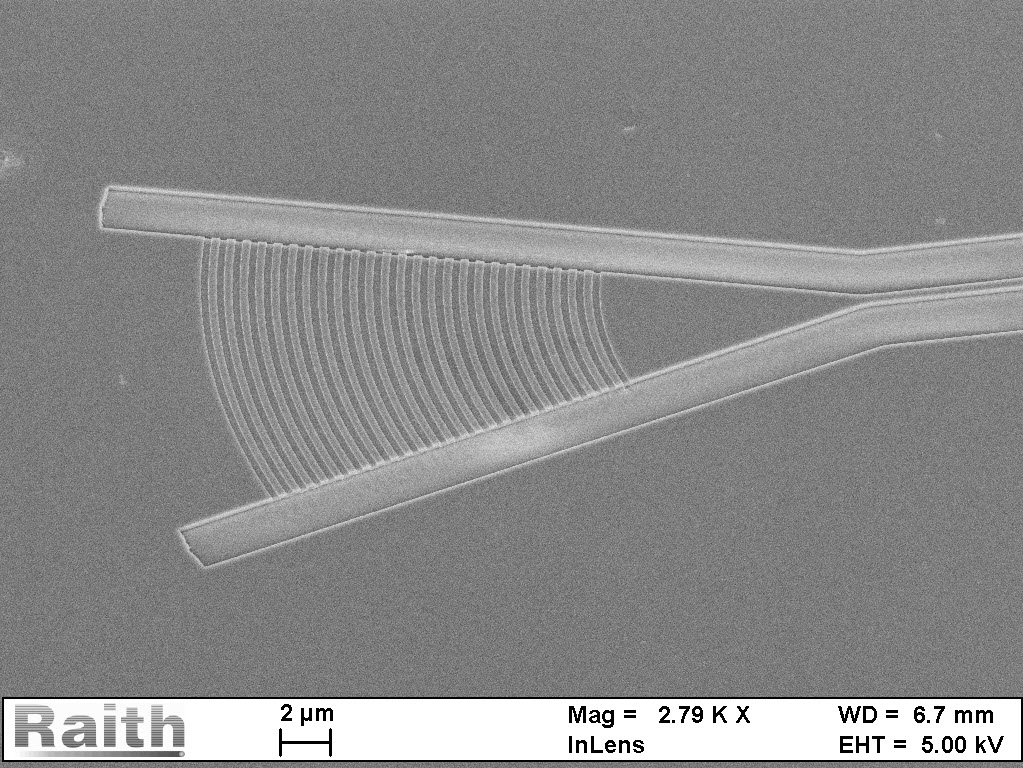
\includegraphics[width=0.7\textwidth]{./Pictures/gratingcoupler.jpg}};
	\node[anchor = north,red,draw,font=\bfseries,yshift=-1.5cm] at (image.center) {220$nm$~SOI刻蚀深度:70$nm$};
\end{scope}
\end{tikzpicture}
\end{frame}

%\begin{frame}{\mbox{SOI}减薄的方法}
%	\begin{columns}
%	\begin{column}[c]{0.6\textwidth}
%		\flushright
%		\begin{tikzpicture}
%			\node[anchor=south west,inner sep=0] (image) at (0,0) {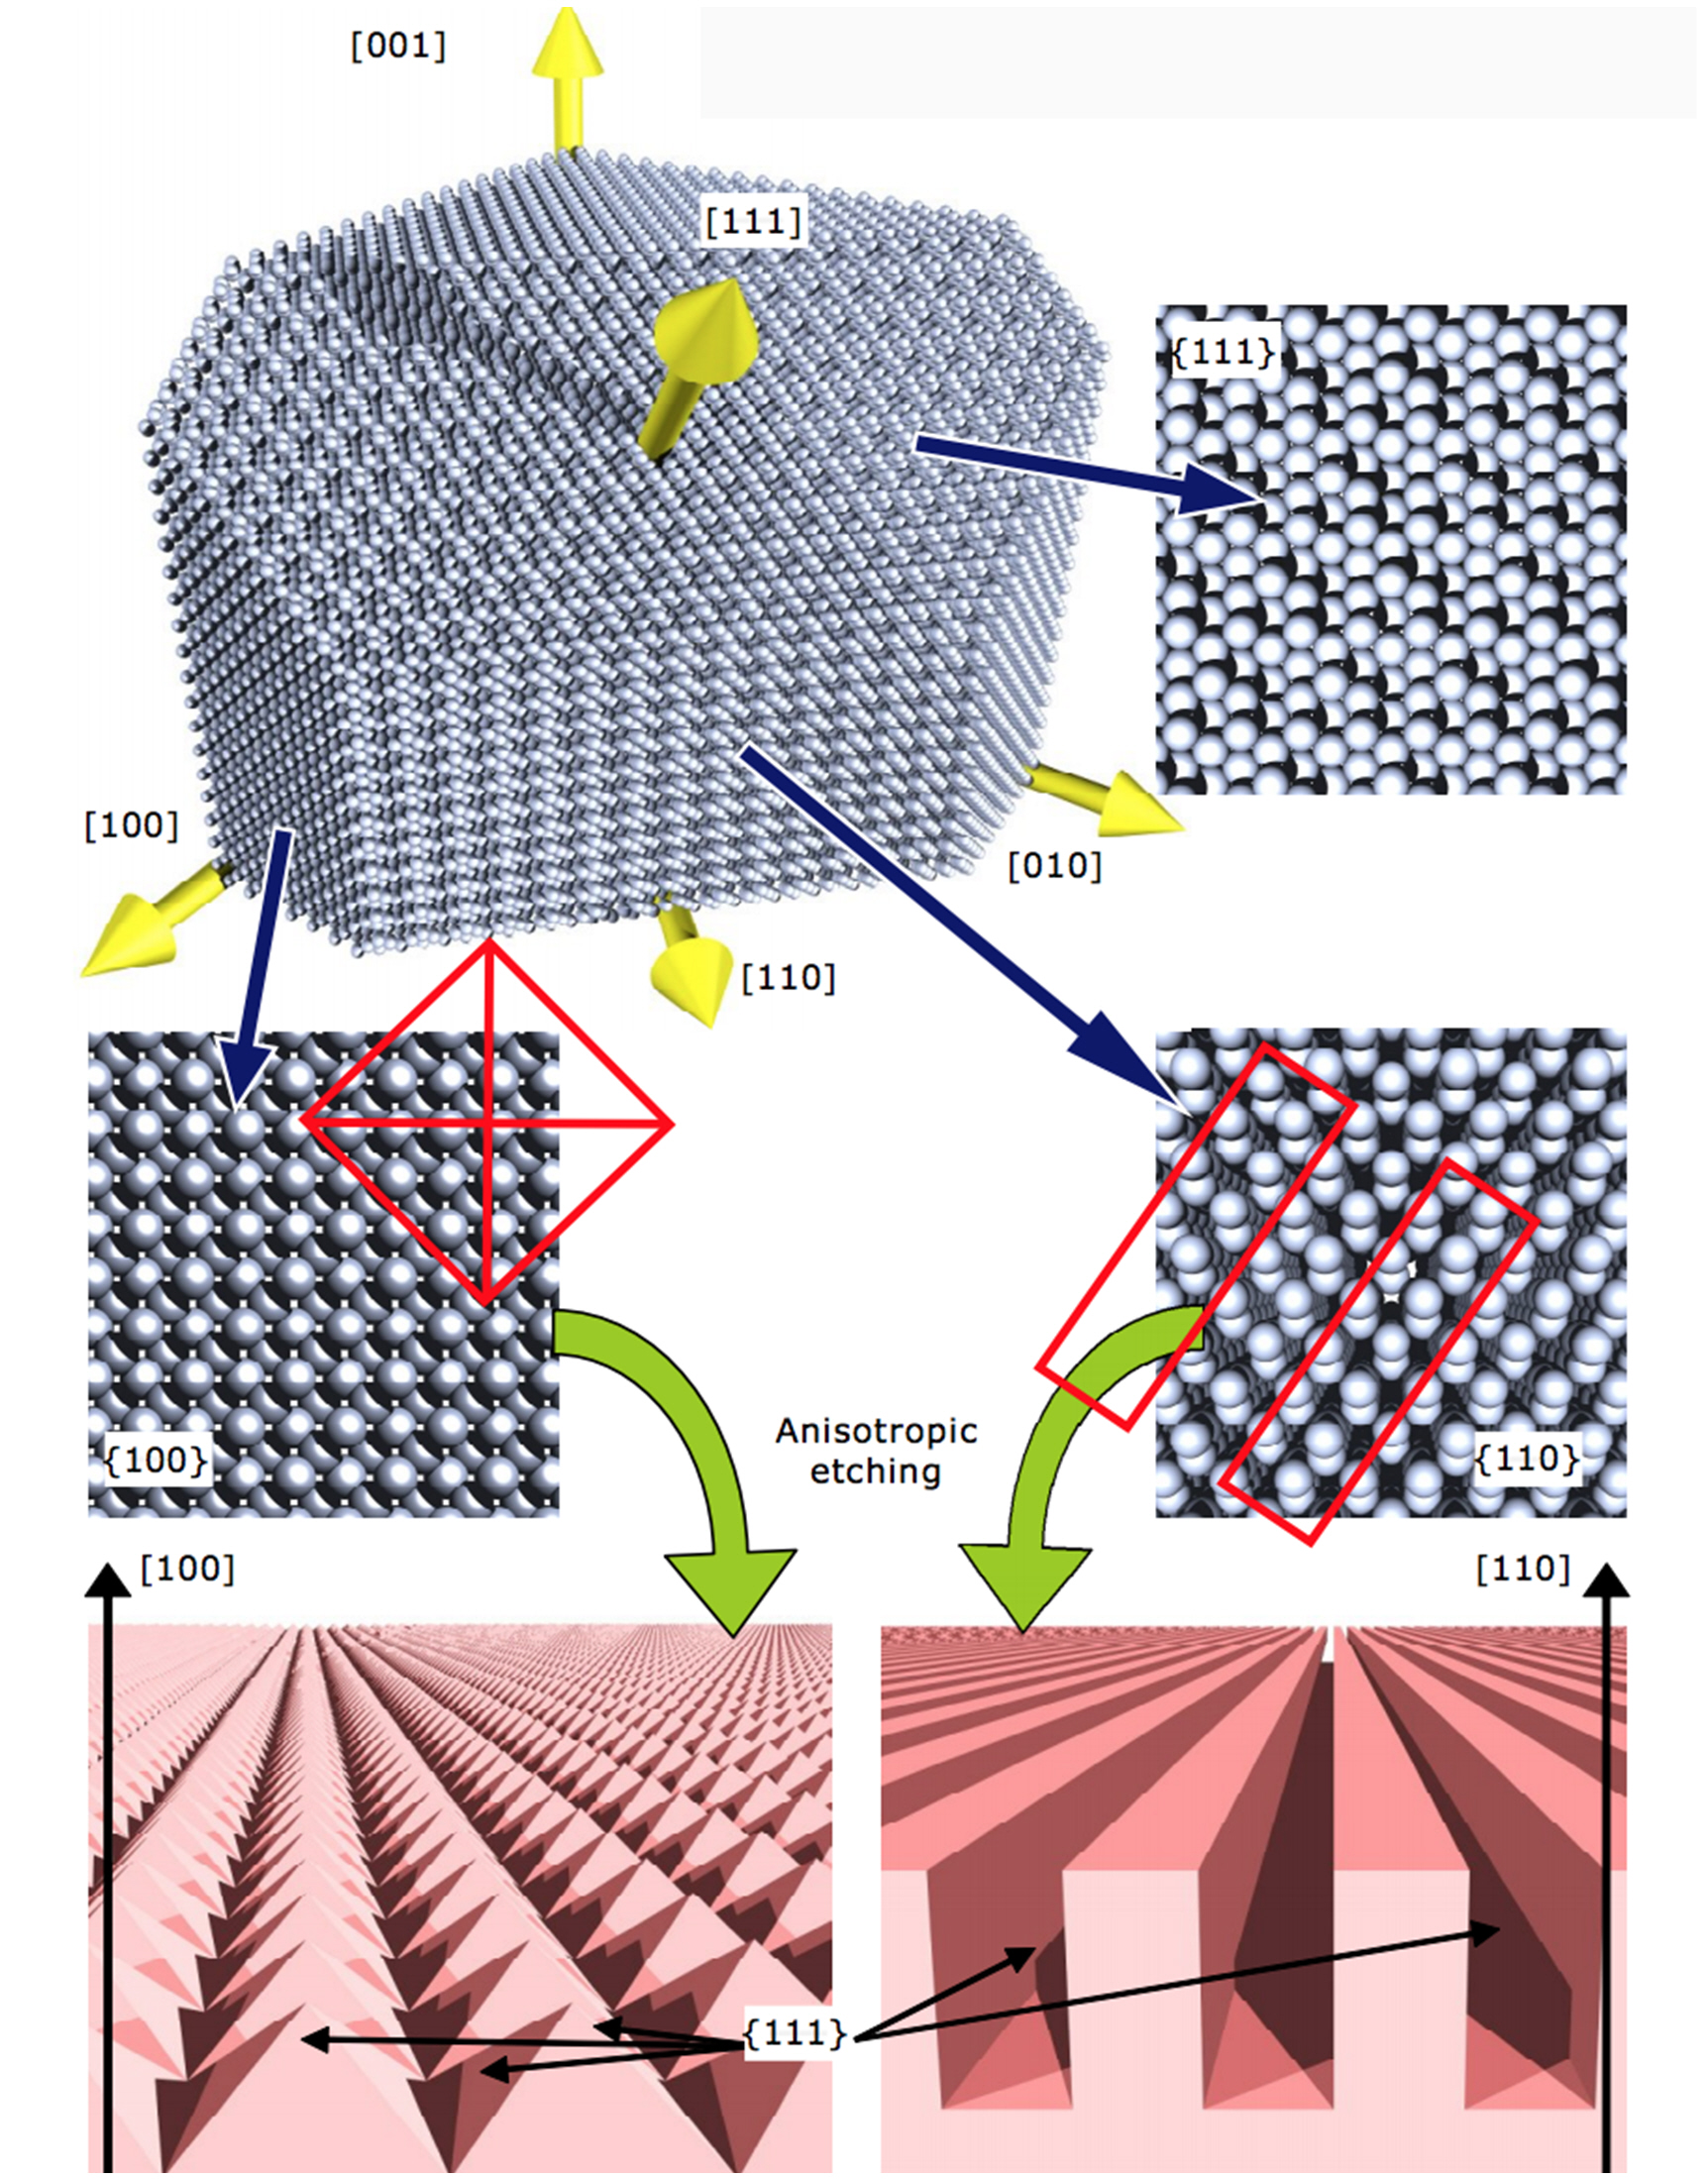
\includegraphics[width=0.8\textwidth]{../Pictures/color_silicon_crystal.jpg}};
%			\begin{scope}[x={(image.south east)},y={(image.north west)}]
%			%\draw[help lines,xstep=.1,ystep=.1] (0,0) grid (1,1); %参考线绘制
%				\node[anchor = center,red,draw,font=\bfseries] at (image.north) {湿法腐蚀};
%			\end{scope}
%		\end{tikzpicture}	
%	\end{column}
%	\begin{column}[c]{0.4\textwidth}
%		\begin{minipage}[c][.6\textheight][c]{\linewidth}
%			\begin{itemize}
%				\item \{111\}:较难腐蚀
%				\item \{100\}:太阳能电池
%				\item \{110\}:微流通道
%			\end{itemize}
%			\onslide+<2>{\zihao{4}\centering\color{red}\bfseries\mbox{ICP}刻蚀\\热氧法}
%		\end{minipage}
%	\end{column}	
%\end{columns}
%\end{frame}

\begin{frame}[t]{光度学与色度学基础}
\centering
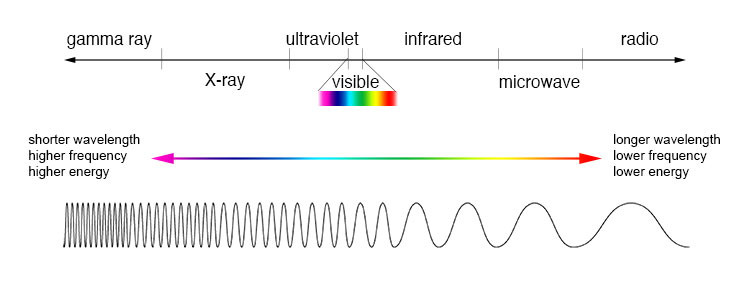
\includegraphics[width=0.9\textwidth]{../Pictures/color_electromagnetic_spectrum.jpg}
\\\vspace{-0.5cm}电磁辐射谱\\
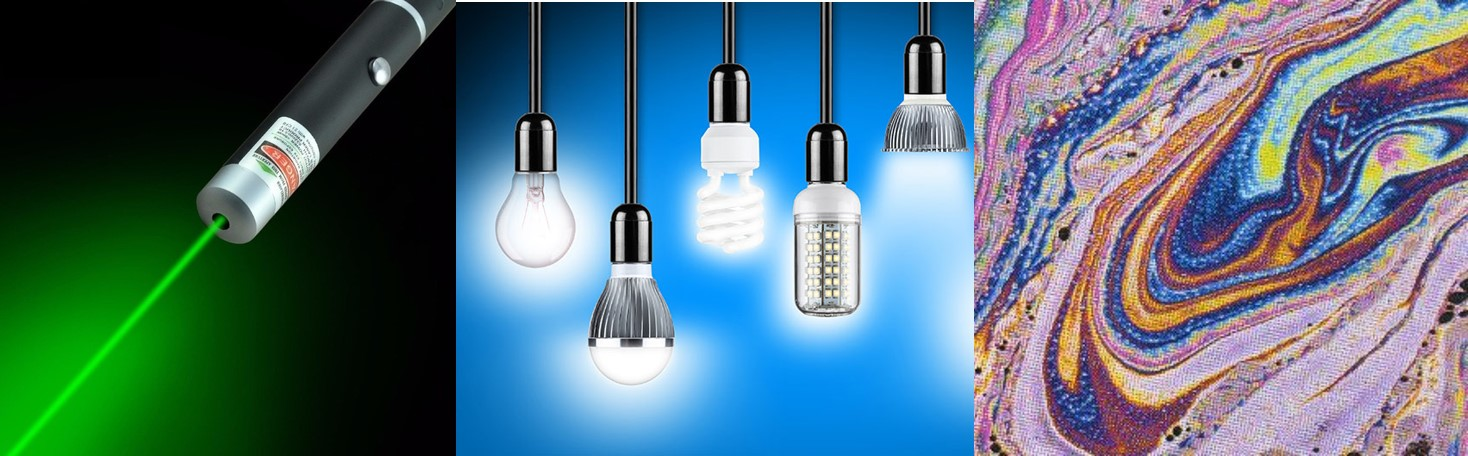
\includegraphics[width=0.9\textwidth]{./Pictures/color.jpg}
\end{frame}

\begin{frame}[t]{光度学与色度学基础}
\uncover<1>{
	\begin{columns}[T] % align columns
		\begin{column}{.48\textwidth}
			\color{red}\rule{\linewidth}{4pt}
			辐射量
			\begin{minipage}[c][.8\textheight][t]{\linewidth}
				\vspace{1cm}
				\begin{itemize}
					\item 辐射能$Q_{e}$
					\item 辐射能通量$\Phi_{e}$
					\item 辐射出射度$M_{e}$
					\item 辐射照度$E_{e}$
				\end{itemize}
			\end{minipage}
		\end{column}%
		\hfill%
		\begin{column}{.48\textwidth}
			\color{blue}\rule{\linewidth}{4pt}
			光学量
			\begin{minipage}[c][.8\textheight][t]{\linewidth}
				\vspace{1cm}
				\begin{itemize}
					\item 光通量$\Phi_{v}$
					\item 光出射度$M_{v}$
					\item 光照度$E_{v}$
					\item 发光强度$I_{v}$
					\item 光亮度$L_{v}$
				\end{itemize}
			\end{minipage}
		\end{column}%
\end{columns}}

\only<2>{
\centering
\vspace{-7cm}
\begin{tikzpicture}
\node[anchor=south west,inner sep=0] (image) at (0,0) {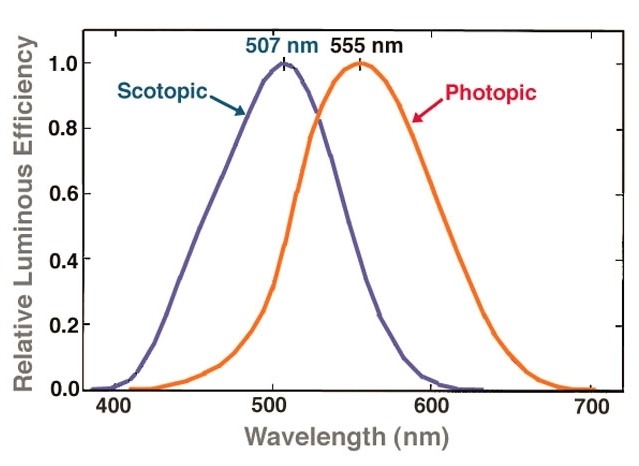
\includegraphics[width=0.8\textwidth]{../Pictures/color_luminous_efficiency.jpg}};
\begin{scope}[x={(image.south east)},y={(image.north west)}]
%\draw[help lines,xstep=.1,ystep=.1] (0,0) grid (1,1); %参考线绘制
	\node[anchor = center,red,draw,font=\bfseries,xshift=2cm] at (image.center) {明视觉};
	\node[anchor = center,red,draw,font=\bfseries,xshift=-2cm] at (image.center) {暗视觉};
\end{scope}
\end{tikzpicture}}
%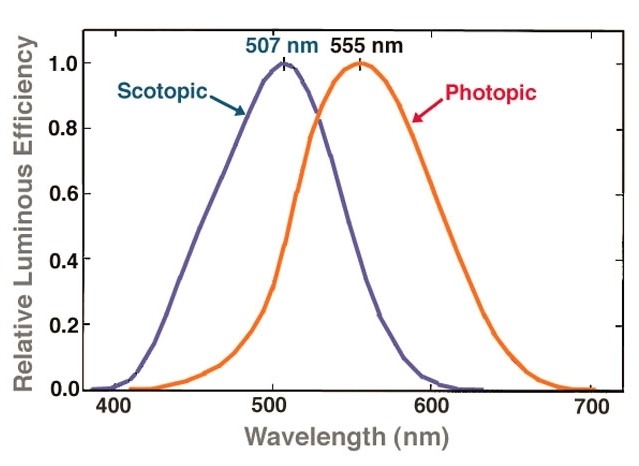
\includegraphics[width=0.7\textwidth]{../Pictures/color_luminous_efficiency.jpg}}
\end{frame}

\begin{frame}[t]{CIE1931-RGB系统}% if there are block, equations in front, you can not move the pictures upward.
\begin{overprint}[\textwidth]
\onslide<1>{
	\begin{minipage}[c][\textheight][t]{\linewidth}
		\begin{block}{}
			\begin{itemize}
				\item 红、绿、蓝三种颜色以不同的量值(有的可能为负值)相混合,可以匹配出任何颜色。
				\item 红、绿、蓝不是唯一的能匹配所有颜色的三种颜色。三种颜色,只要其中的每一种都不能用其他两种混合产生出来,就可以用它们匹配所有的颜色。
			\end{itemize}
		\end{block}
		\centering\vspace{0.5cm}
		{\zihao{4}\color{red}\bfseries 颜色匹配函数}
		\begin{equation*}
			\zihao{4}
			C(\lambda)\equiv\overline{r}(\lambda)+\overline{g}(\lambda)+\overline{b}(\lambda)			
		\end{equation*}
	\end{minipage}}
%a line is need, otherwise the picture will be on the right.

\onslide+<2->{
	\centering
	\vspace{-7.5cm}
	\begin{tikzpicture}
		\node[anchor=south west,inner sep=0] (image) at (0,0) {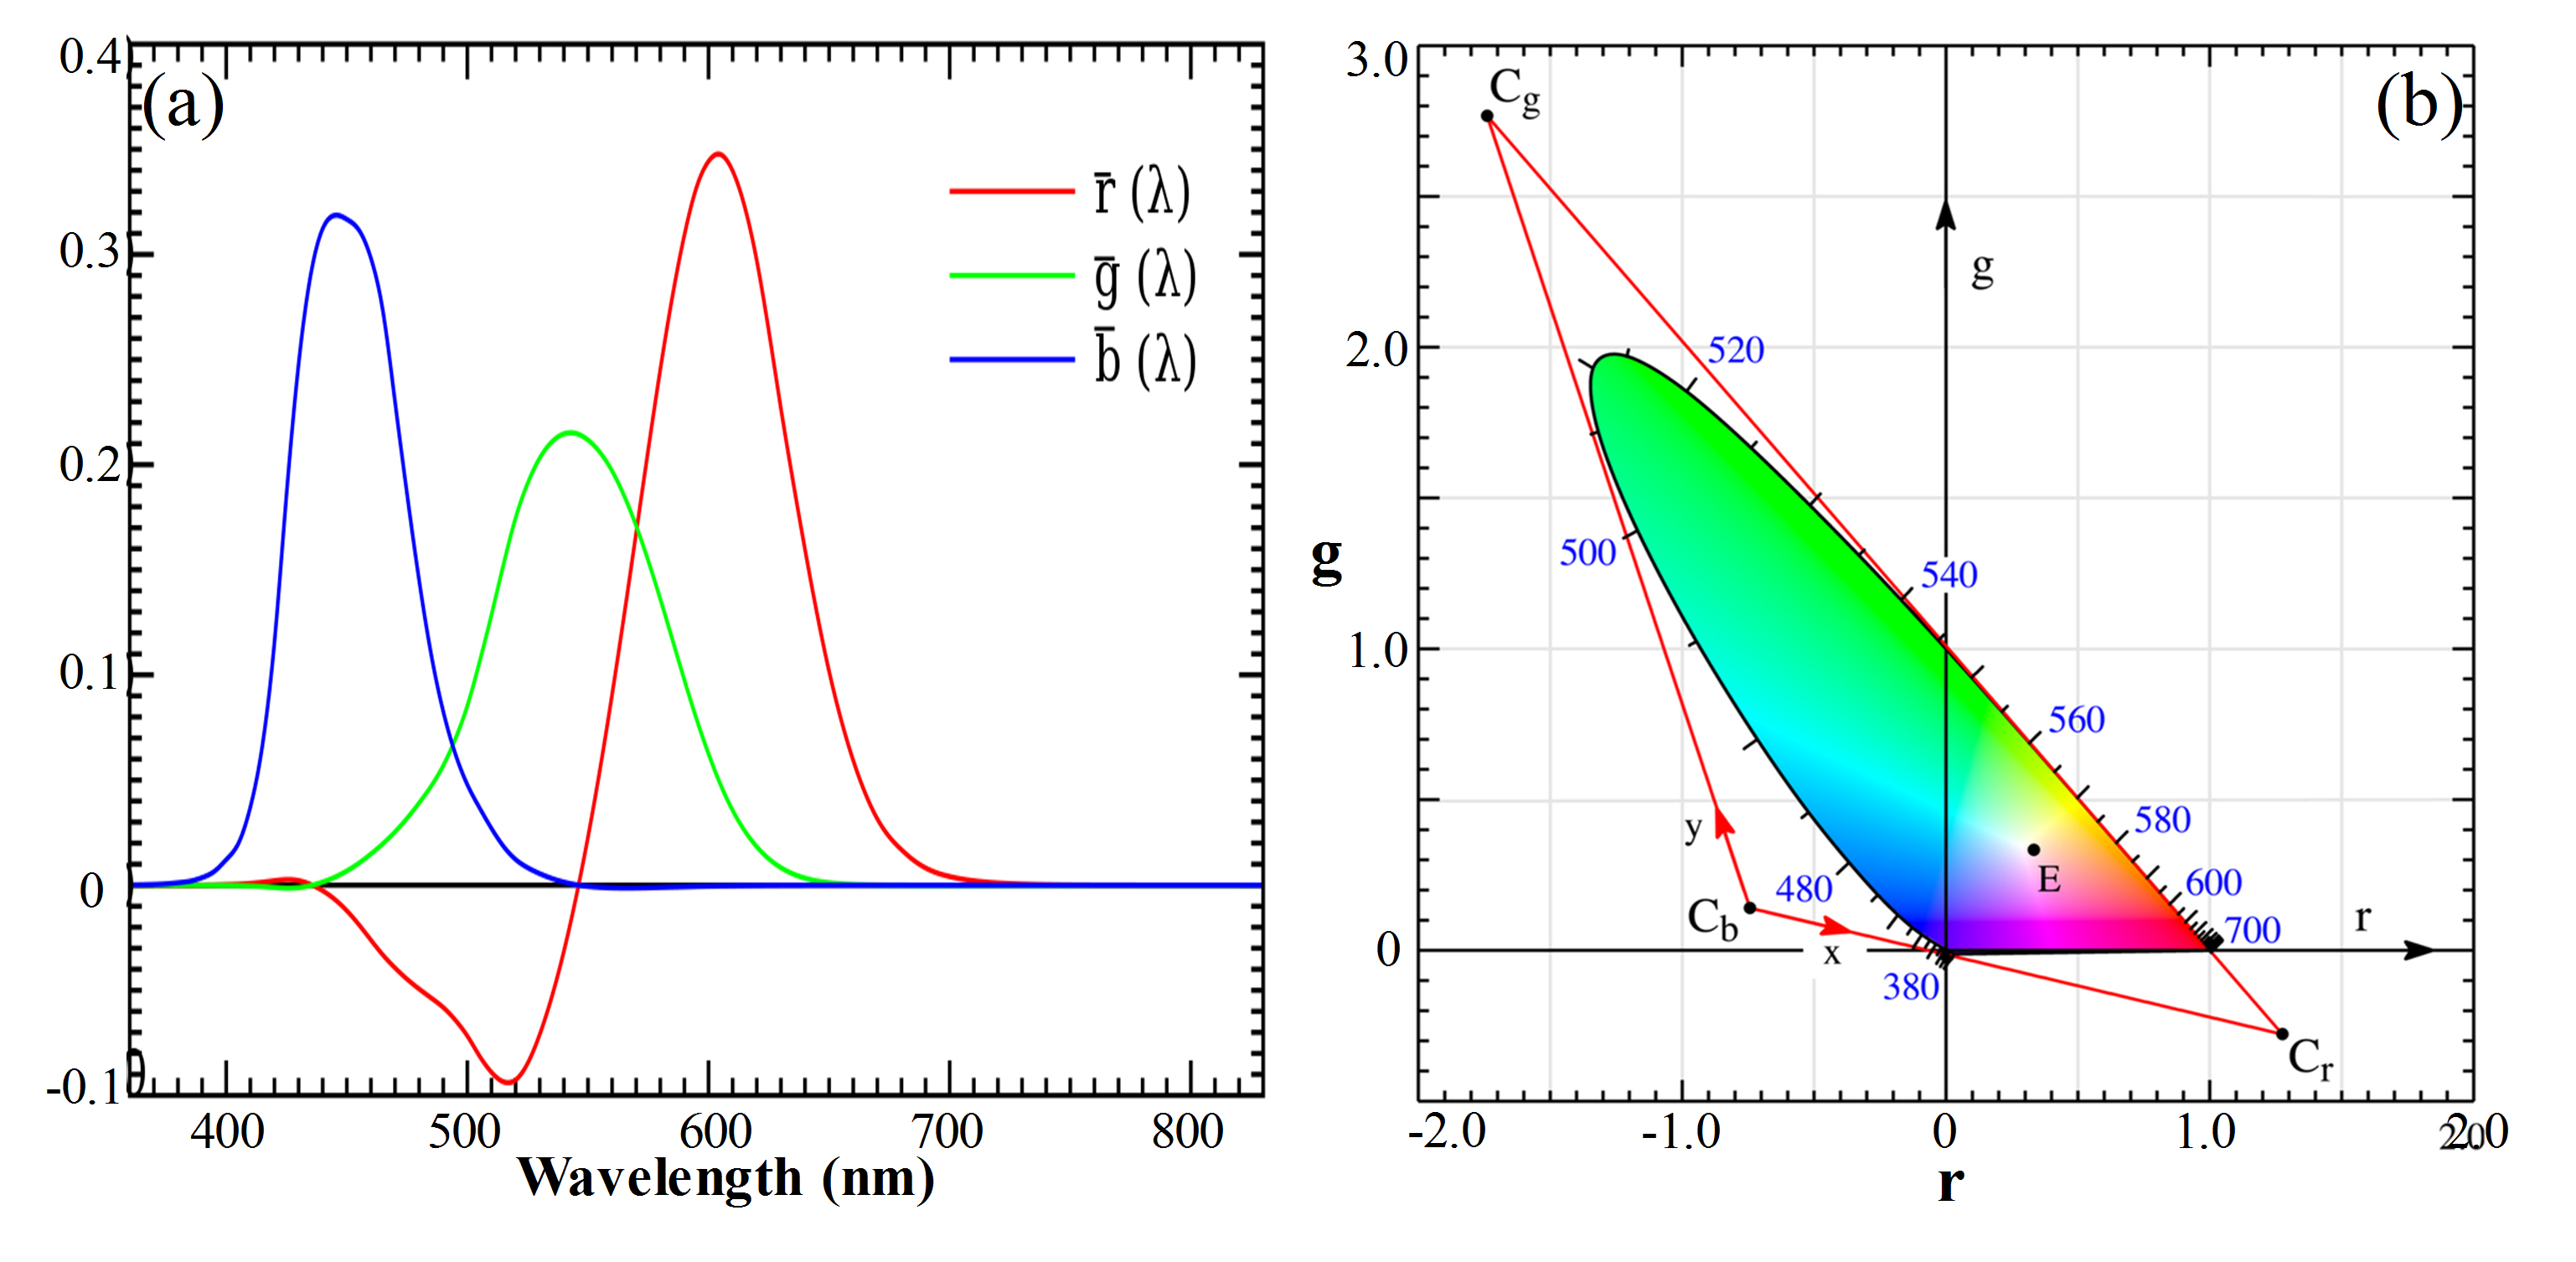
\includegraphics[width=\textwidth]{../Pictures/color_rgb_combined.jpg}};
		\begin{scope}[x={(image.south east)},y={(image.north west)}]
			%\draw[help lines,xstep=.1,ystep=.1] (0,0) grid (1,1); %参考线绘制
		\only<3>{\node[anchor = center,red,draw,font=\bfseries] at (0.7,0.8) {负值};}
		\end{scope}
	\end{tikzpicture}}
%	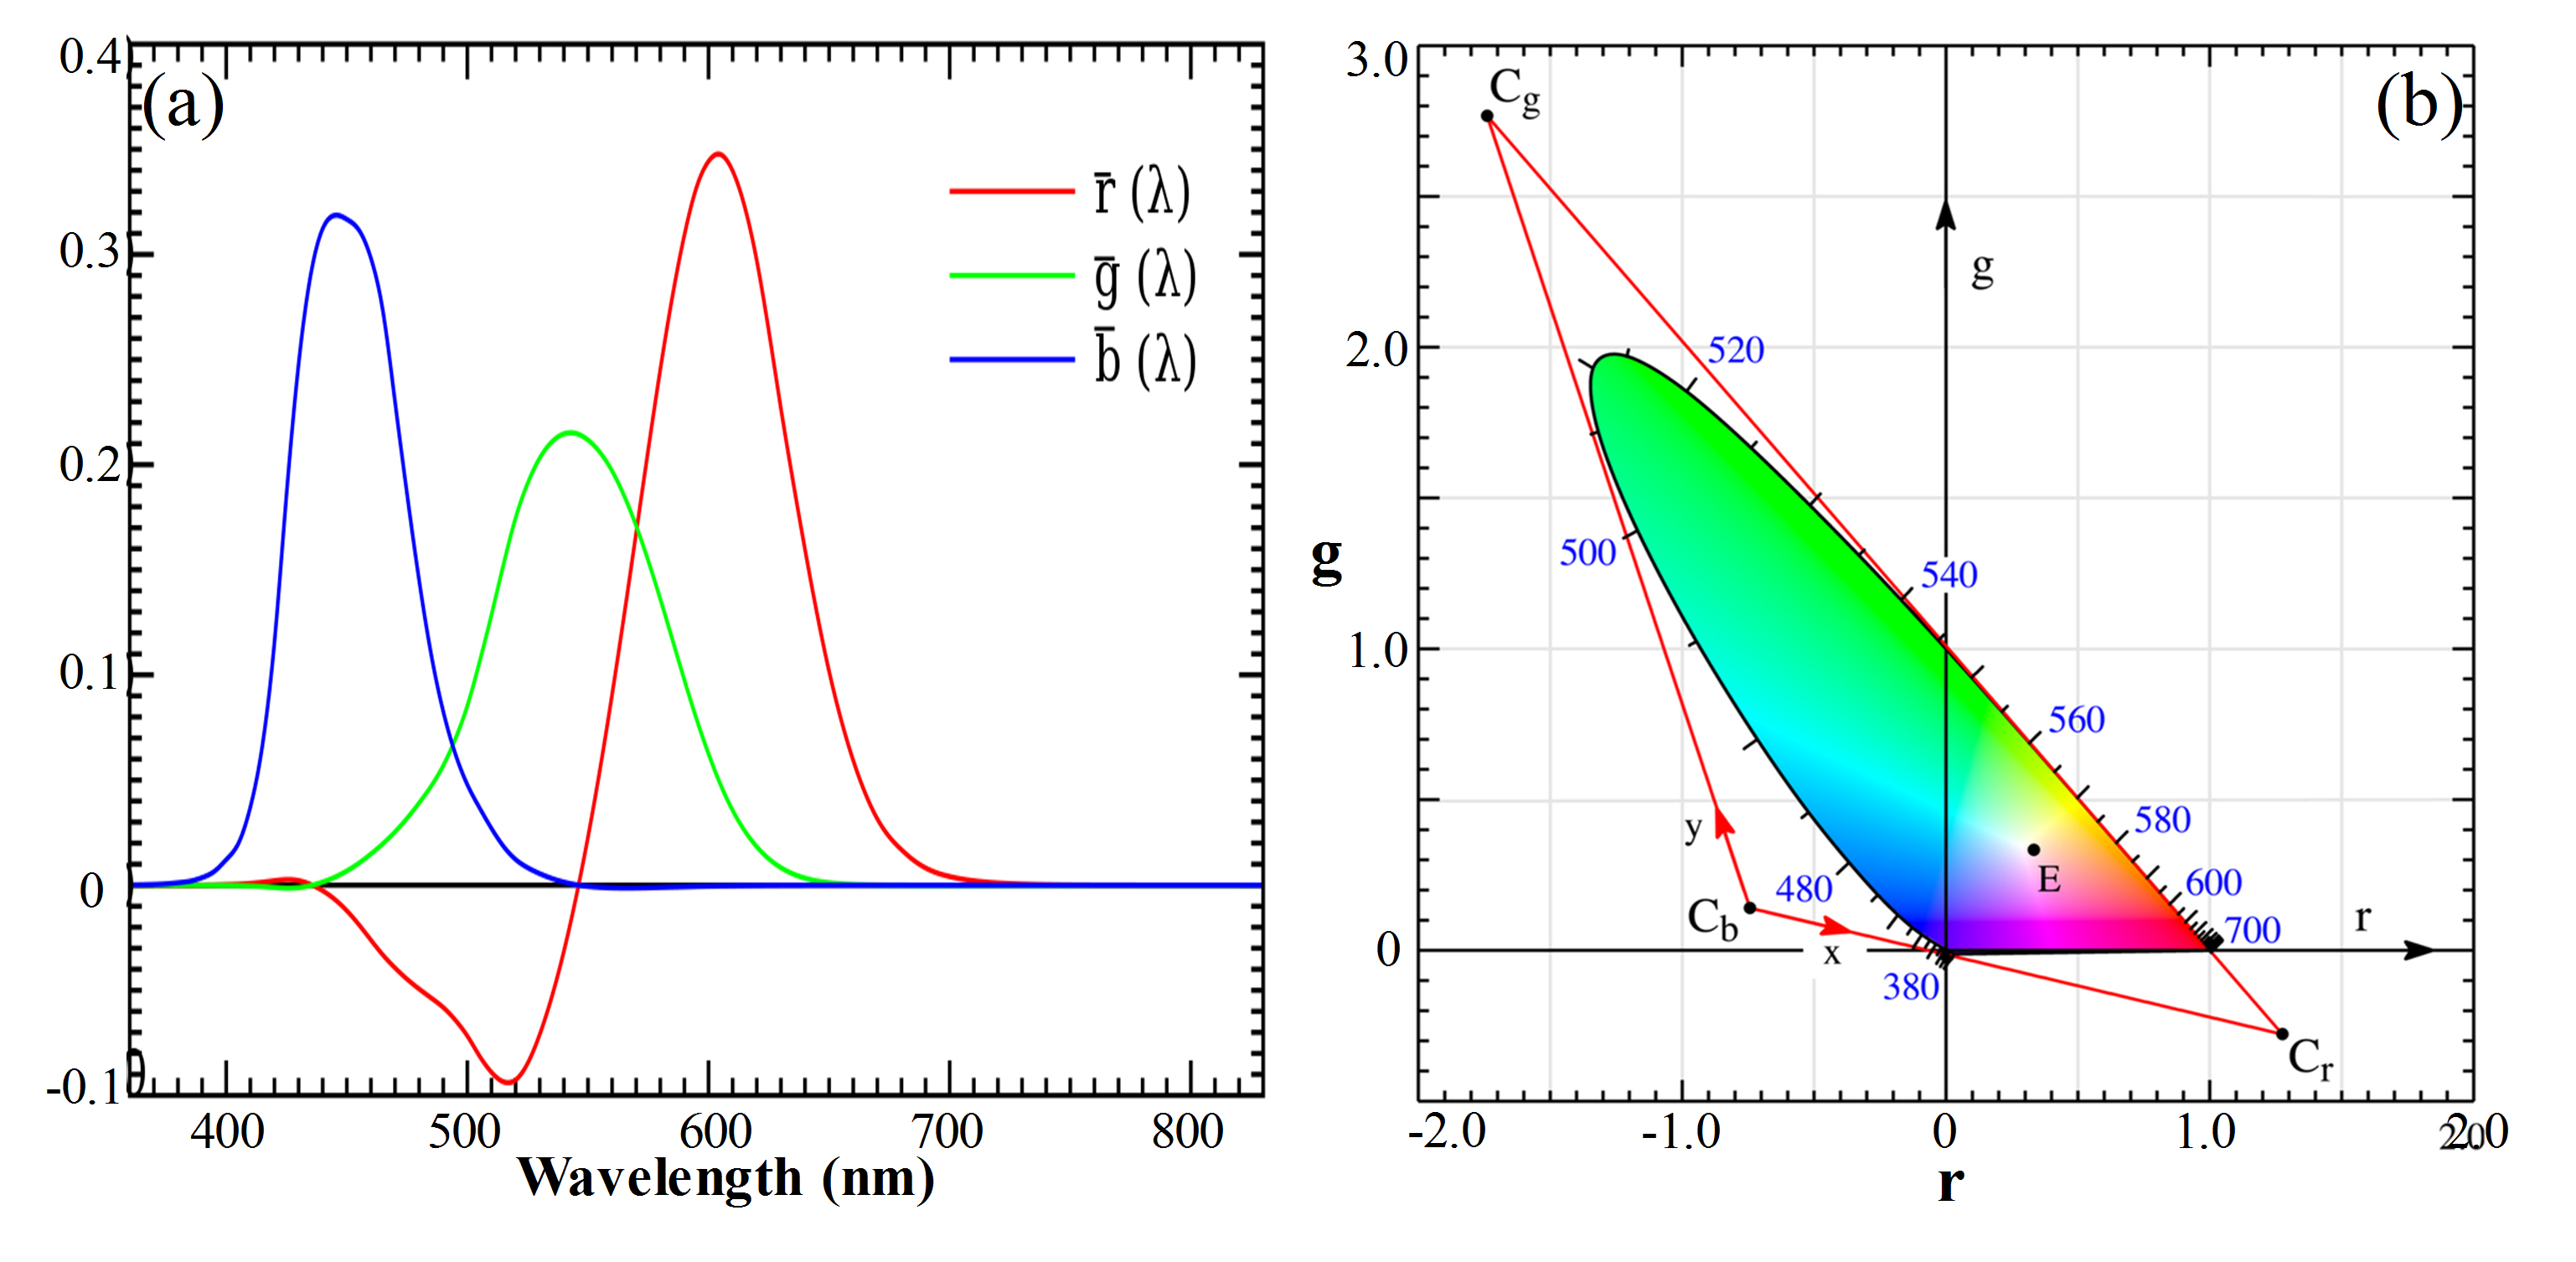
\includegraphics[width=\textwidth]{../Pictures/color_rgb_combined.jpg}}
\end{overprint}
\end{frame}

\begin{frame}{CIE1931-XYZ系统}
\begin{overprint}[\textwidth]
	\onslide<1>{
		\begin{minipage}[c][\textheight][t]{\linewidth}
			\begin{block}{X、Y、Z三原色选取规则}
				\begin{itemize}
					\item 用此三原色匹配等能光谱色,三刺激值不应出现负值。
					\item 实际不存在的颜色在色品图上所占的面积应尽量小。
					\item 用Y刺激值表示颜色的亮度,同时亦表示色度;而X和Z刺激值只表示色度,不代表亮度。
				\end{itemize}
			\end{block}
			\centering
			\begin{tabular}[t]{|cccc|}
				\hline
				& r & g & b  \\
				\hline
				(X) & 1.2750 & -0.2778 & 0.0028  \\
				\hline
				(Y)	& -1.7392 & 2.7671 & -0.0279  \\
				\hline
				(Z)	& -0.7431 & 0.1409 & 1.6022  \\
				\hline
			\end{tabular}
	\end{minipage}}
	%a line is need, otherwise the picture will be on the right.
	
	\onslide+<2>{
		\centering
		\vspace{-8cm}
		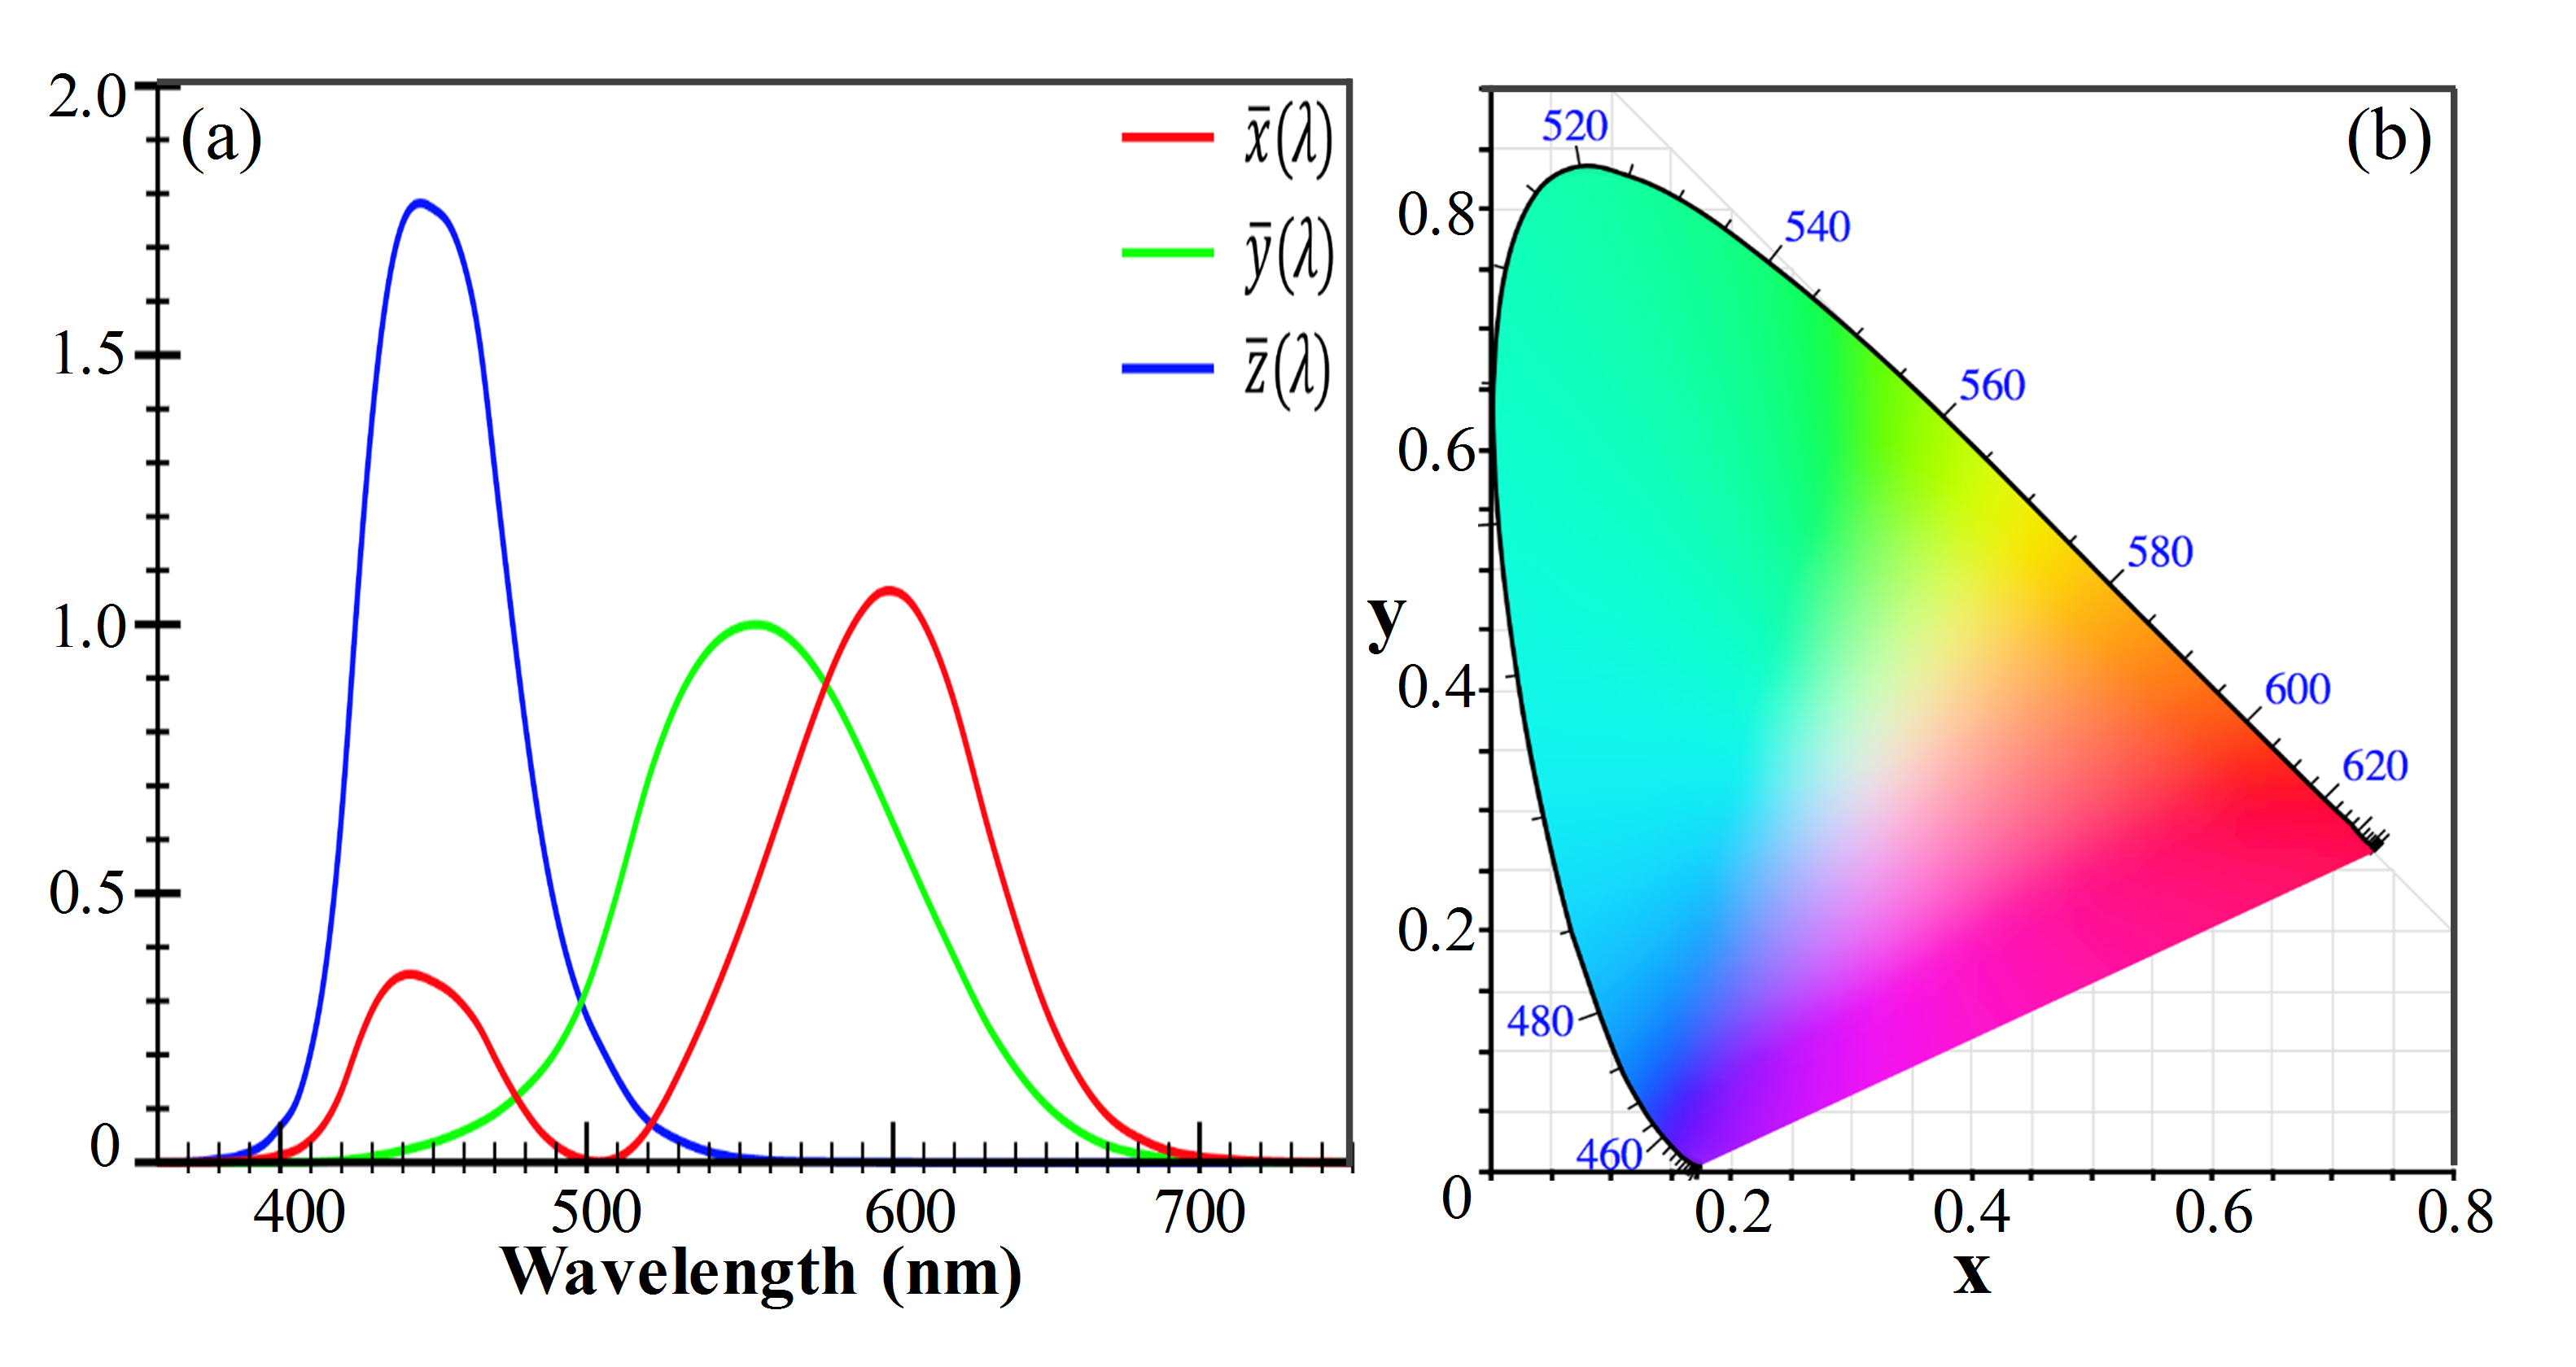
\includegraphics[width=\textwidth]{../Pictures/color_xyz_combined.jpg}}
\end{overprint}
\end{frame}

\begin{frame}[t]{XYZ坐标与RGB坐标的转换}
\begin{columns}
	\begin{column}[c]{0.35\textwidth}
		\begin{tikzpicture}
		\node[anchor=south west,inner sep=0] (image) at (0,0) {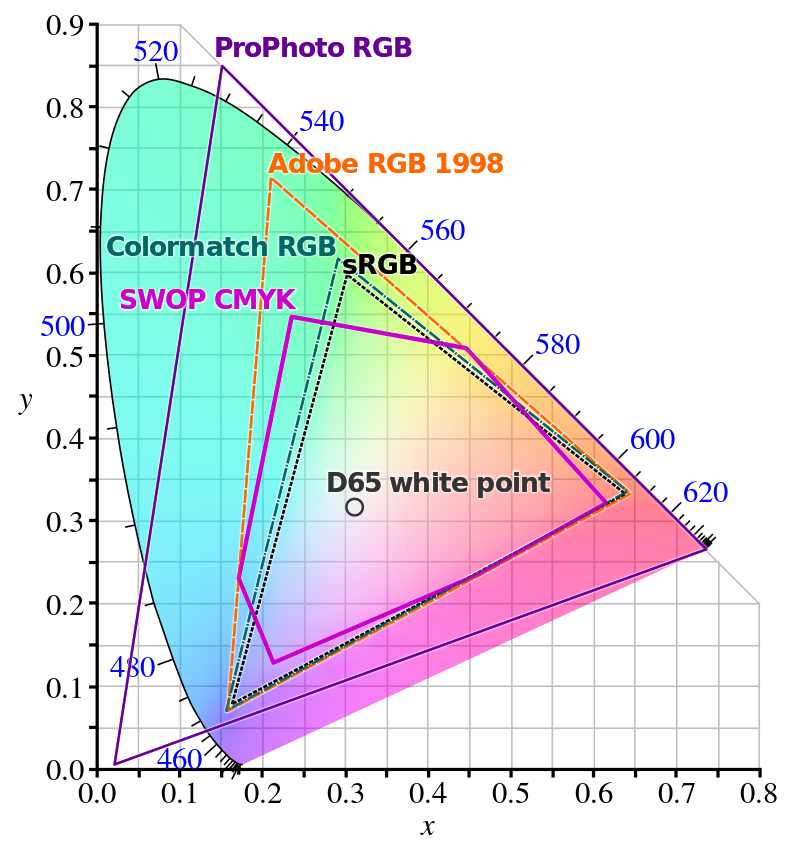
\includegraphics[width=1.1\textwidth]{./Pictures/different_rgb.png}};
		\end{tikzpicture}	
	\end{column}
	\begin{column}[c]{0.65\textwidth}
		\begin{minipage}[c][0.8\textheight][c]{\linewidth}
			\small\centering
			\mbox{\mbox{sRGB}三原色与参考白\mbox{xyY}坐标点}
			\begin{tabular}[t]{|ccccc|}
				\hline
				& Red & Green & Blue & White point \\
				\hline
				x & 0.6400 & 0.3000 & 0.1500 & 0.3127 \\
				\hline
				y	& 0.3300 & 0.6000 & 0.0600 & 0.3290 \\
				\hline
				Y	& 0.2126 & 0.7152 & 0.0722 & 1.0000 \\
				\hline
			\end{tabular}
		\begin{equation*}
			\left[\begin{array}{c}
			R\\G\\B
			\end{array}
			\right]=
			\begin{bmatrix}
			3.2406 & -1.5372 & -0.4986\\
			-0.9689 & 1.8758 & 0.0415\\
			0.0557 & -0.2040 & 1.570
			\end{bmatrix}
			\begin{bmatrix}
			X\\Y\\Z
			\end{bmatrix}
		\end{equation*}
		\begin{equation*}
			c_{srgb} = \left\{
			\begin{array}{lcc}
			12.92c_{rgb}, &     & c_{rgb}\le0.0031308\\
			(1+a)c_{rgb}^{1/2.4}-a,&     & c_{rgb}>0.0031308
			\end{array}
			\right.
		\end{equation*}
		\end{minipage}
	\end{column}	
\end{columns}
\end{frame}

\begin{frame}{\mbox{SOI}色谱图的计算}
	\centering
	\only<1>{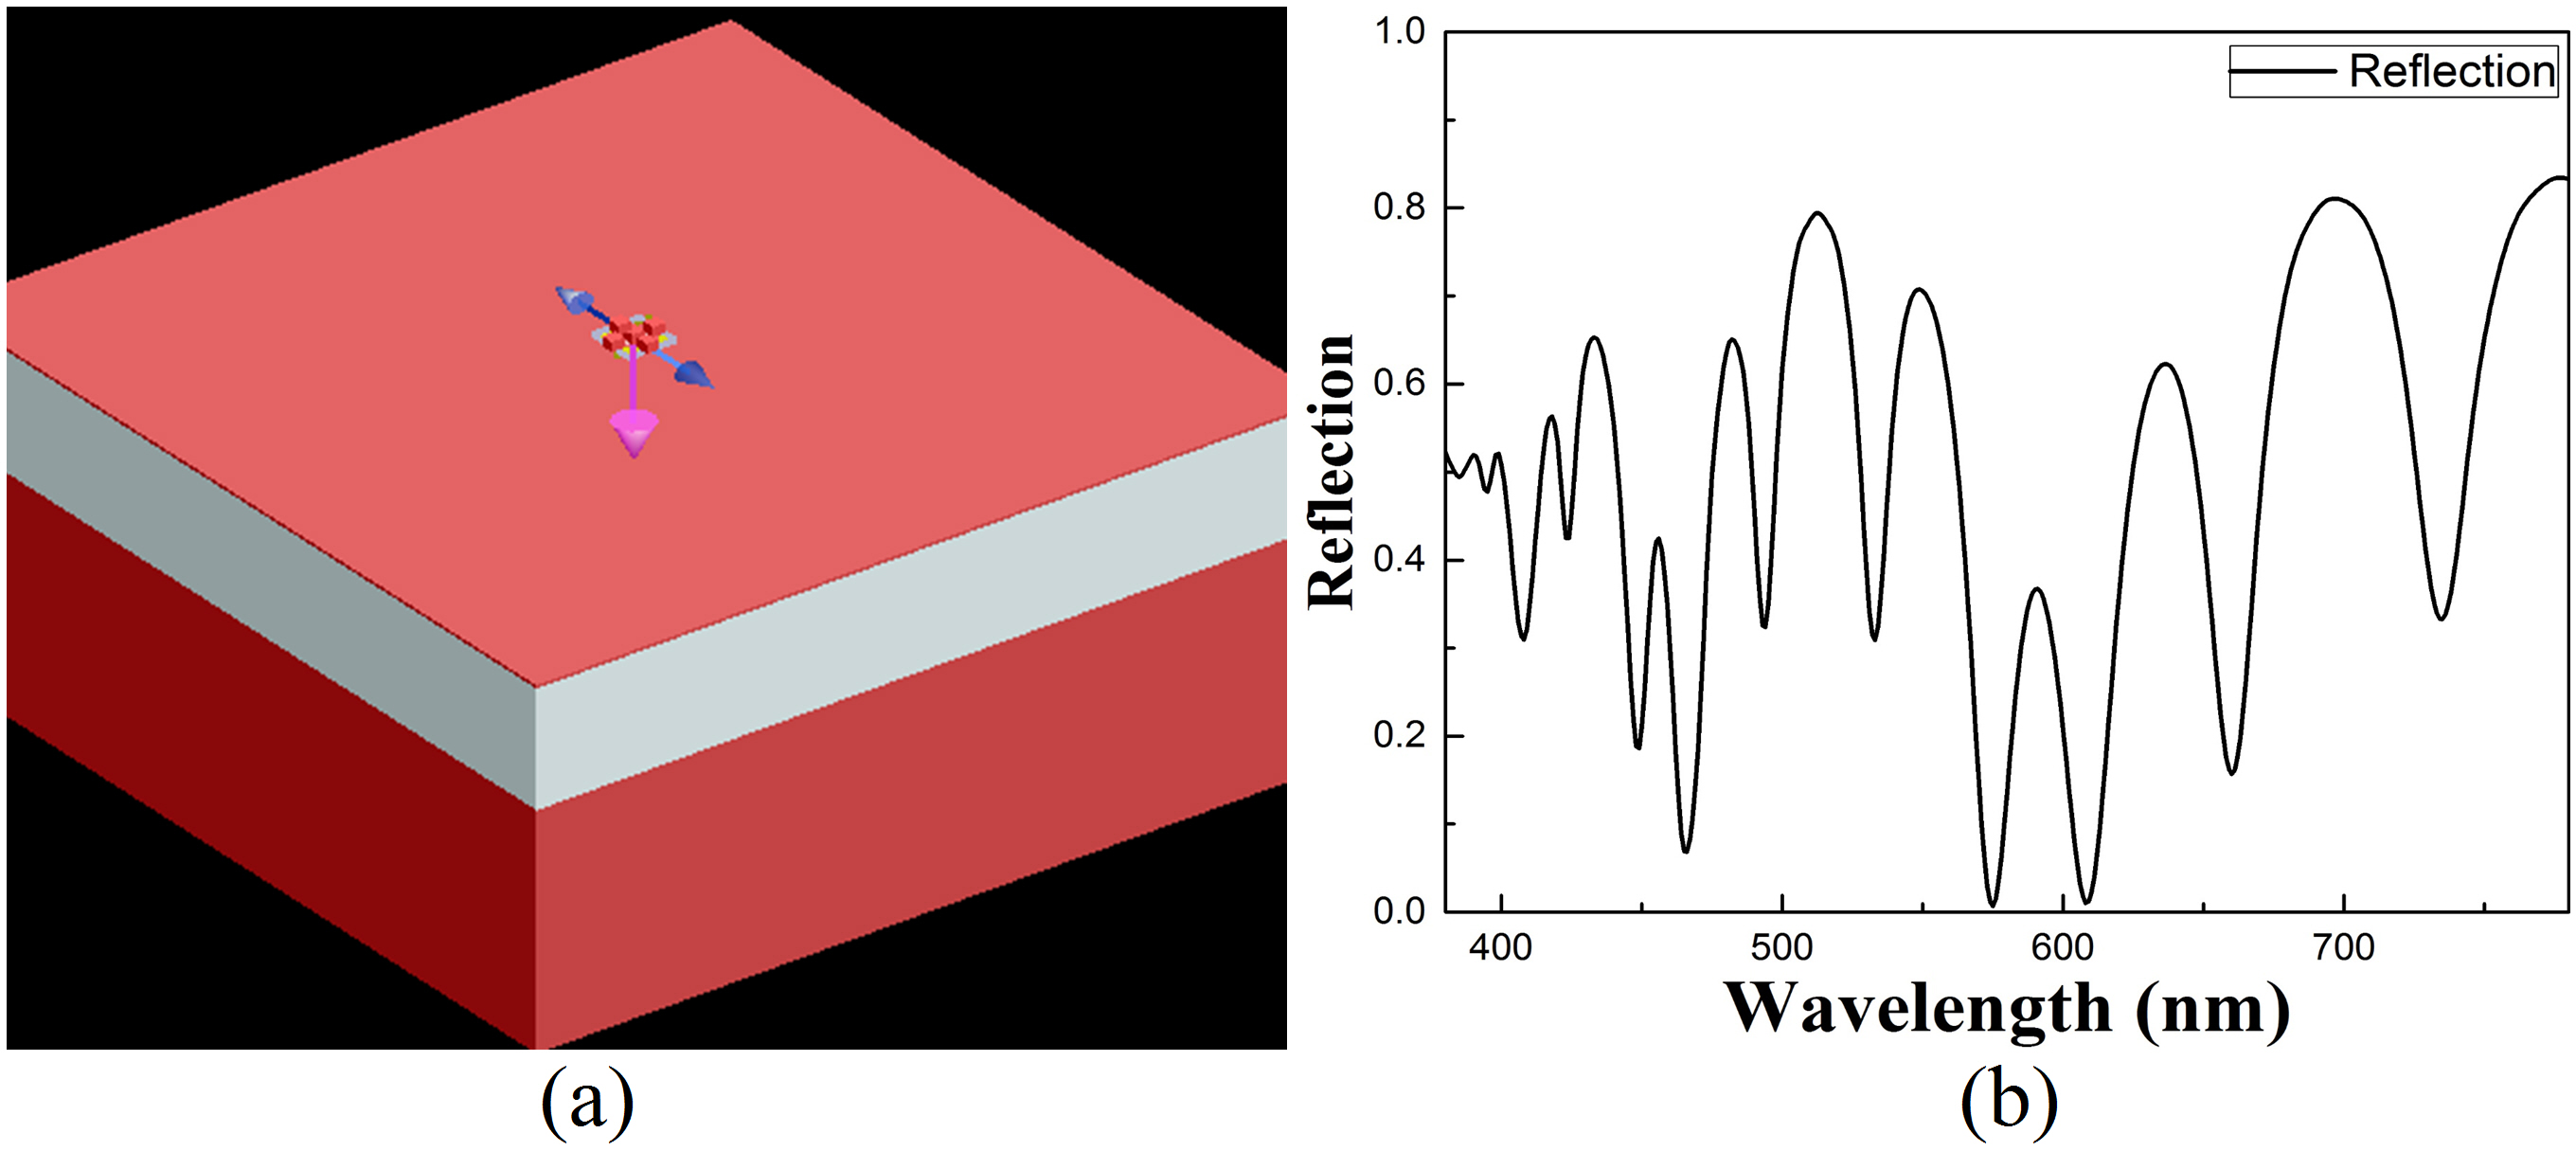
\includegraphics[width=\textwidth]{../Pictures/color_reflection.jpg}\\\hspace{0.5cm}{\centering\zihao{4}\bfseries 仿真模型}}
	\only<2>{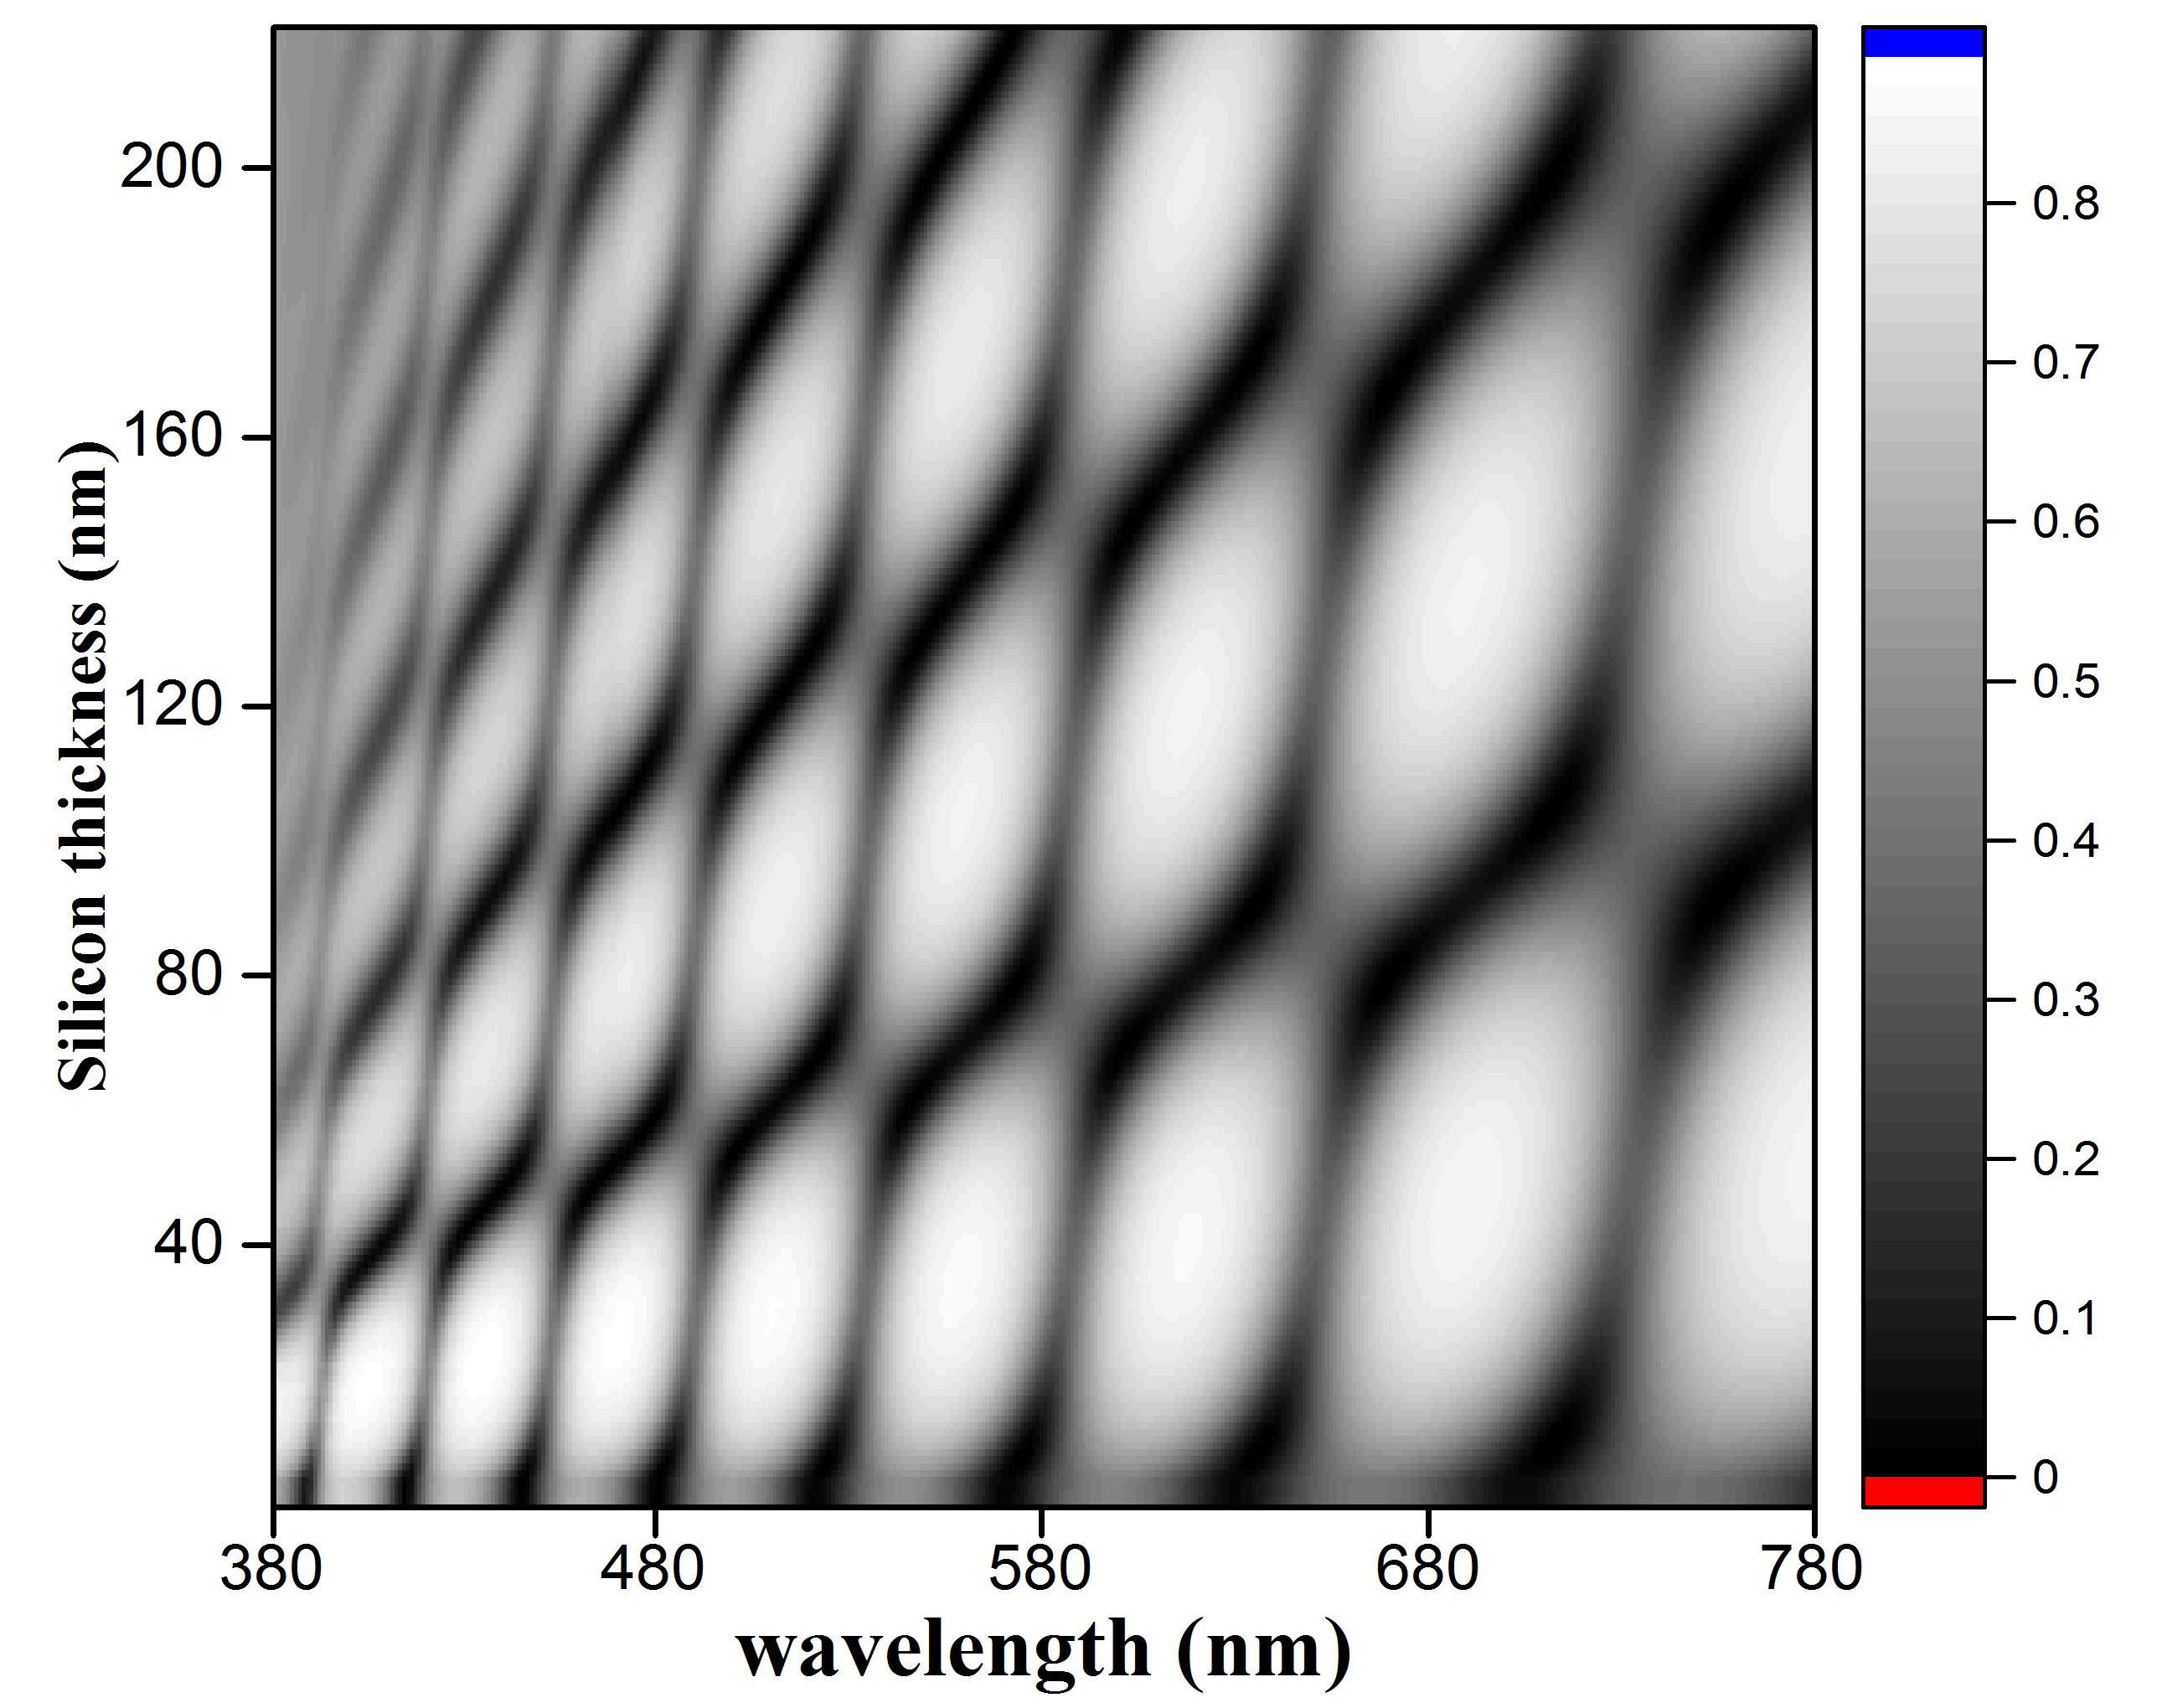
\includegraphics[width=0.7\textwidth]{../Pictures/color_reflection_all.jpg}\\\hspace{0.7cm}{\centering\zihao{4}\bfseries 不同硅层厚度下的反射率}}
	\only<3>{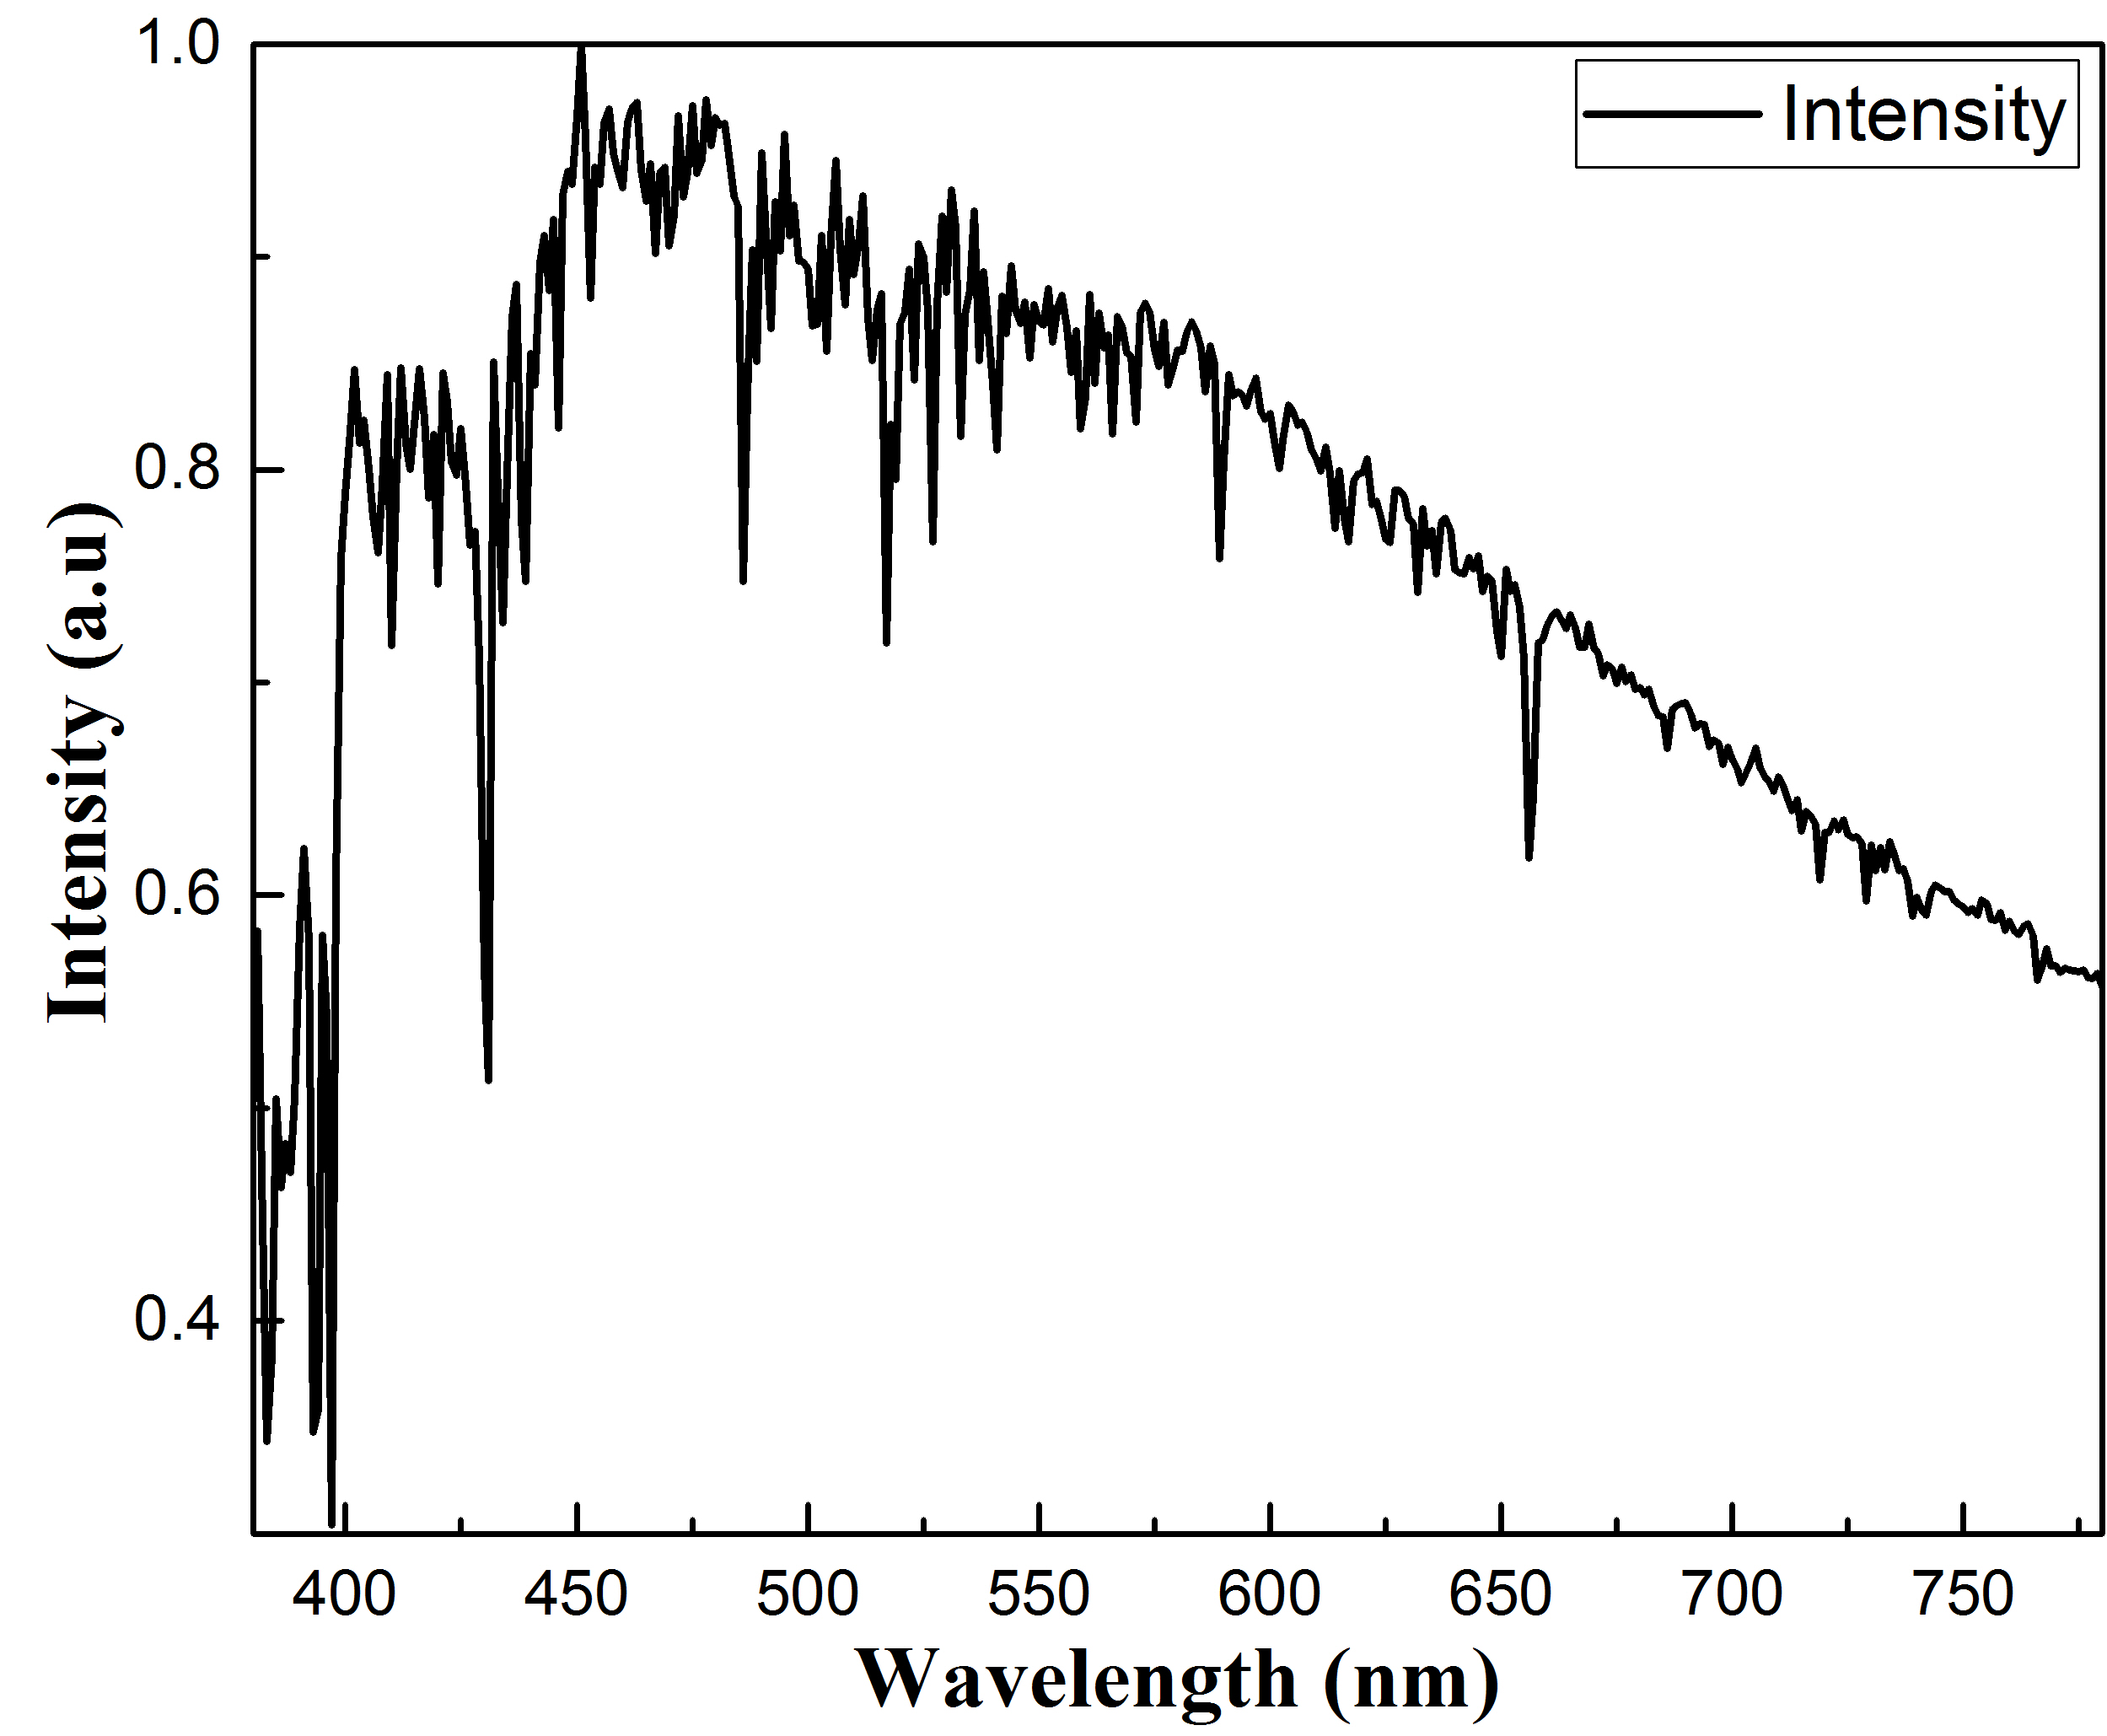
\includegraphics[width=0.7\textwidth]{../Pictures/color_sun_spectrum.jpg}\\\hspace{1cm}{\centering\zihao{4}\bfseries 太阳光谱\mbox{(from NREL)}}}
	\only<4>{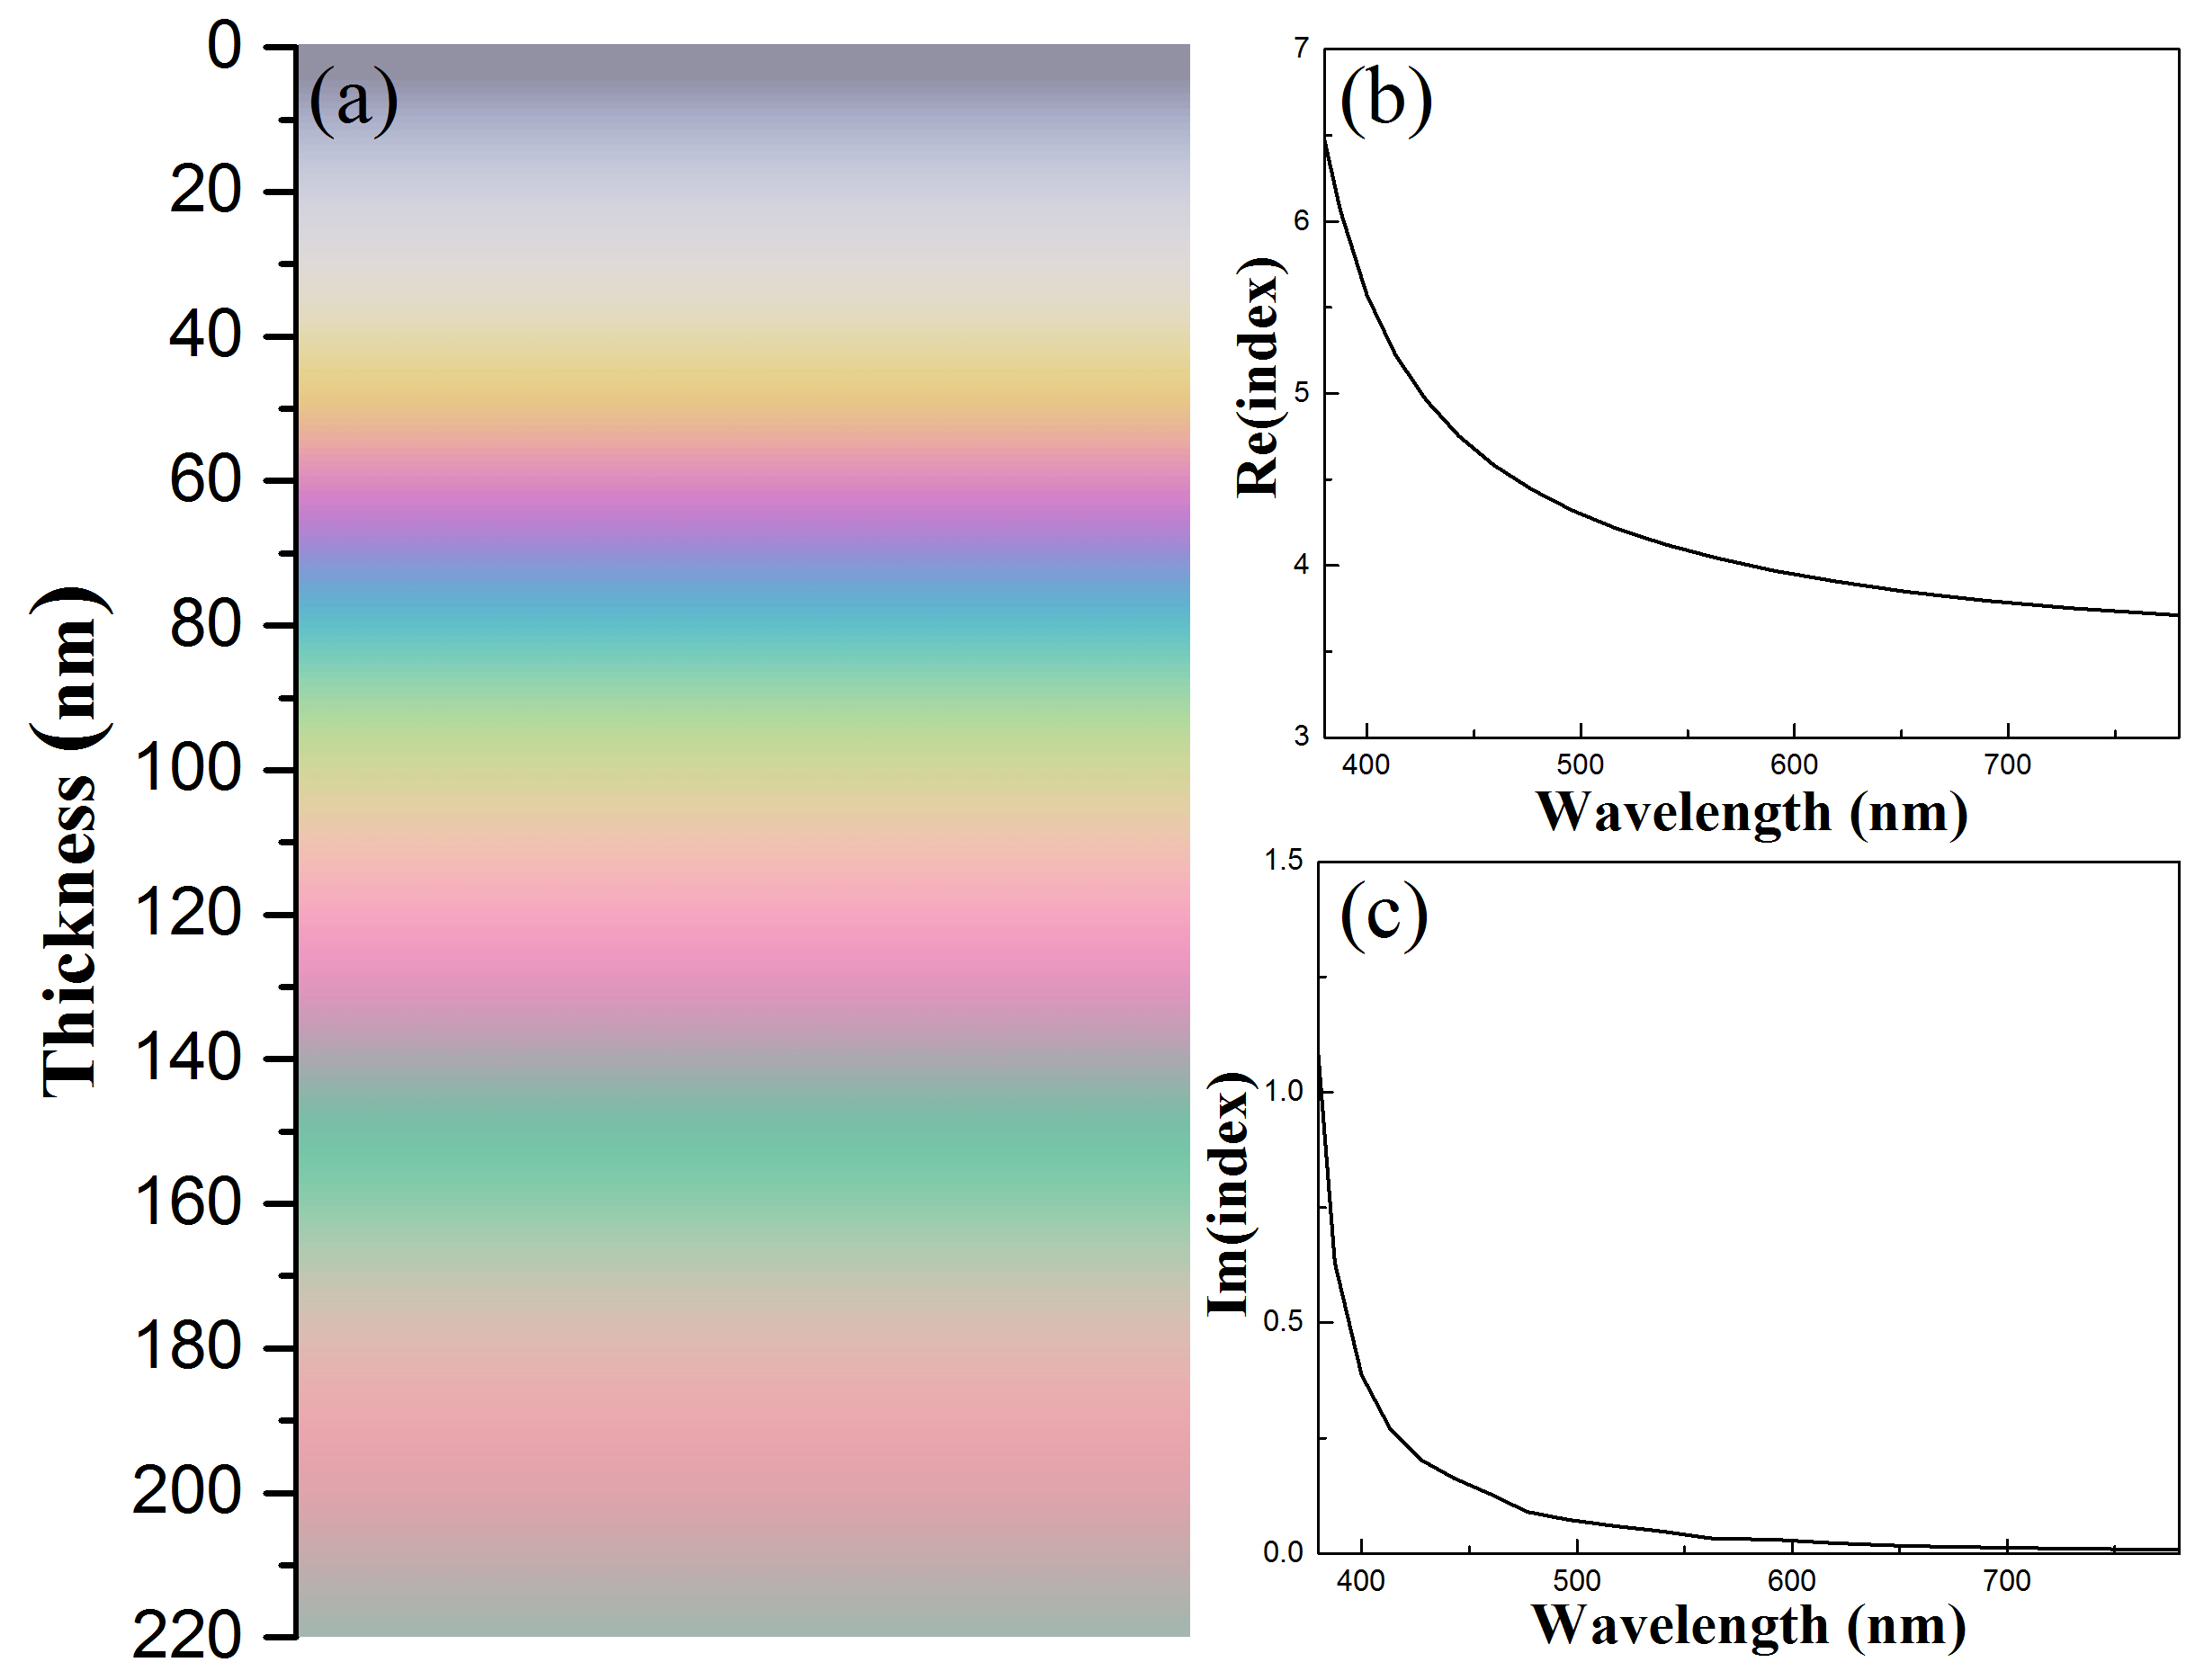
\includegraphics[width=0.8\textwidth]{../Pictures/color_220nm.jpg}\\\hspace{-2.8cm}{\centering\bfseries \mbox{SOI}芯片色谱图}}
	\only<5>{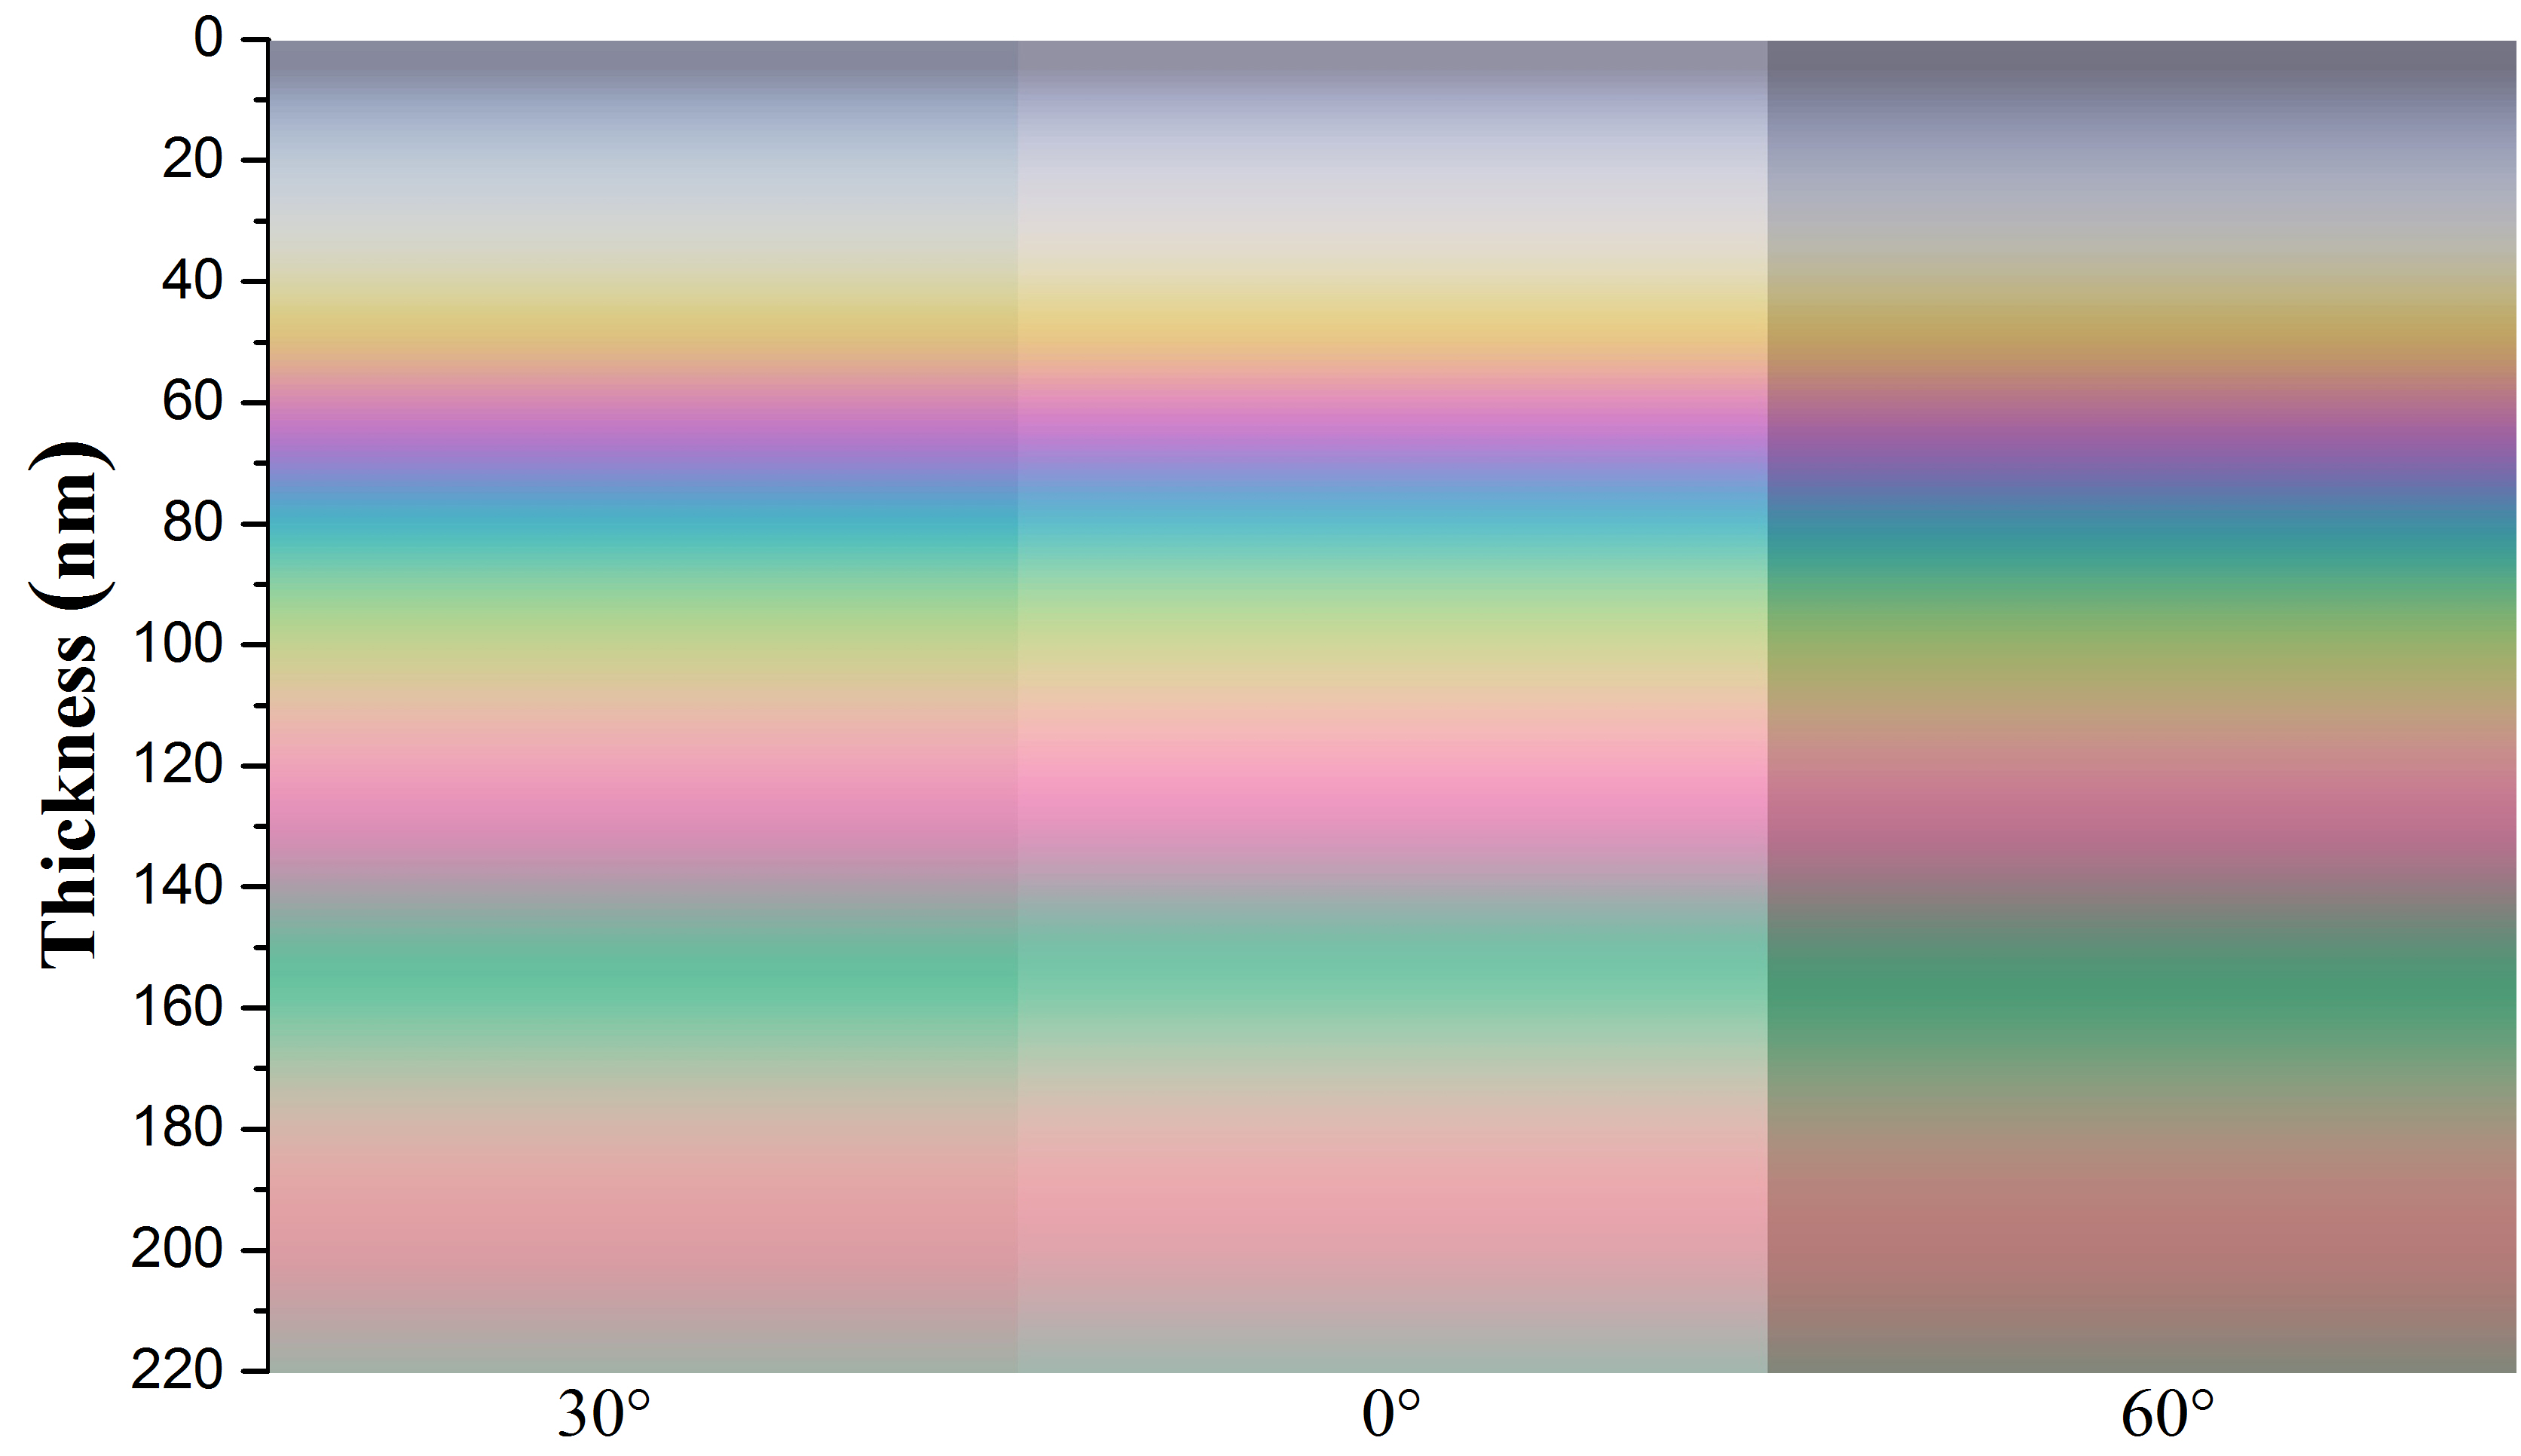
\includegraphics[width=0.9\textwidth]{../Pictures/color_compare.jpg}\\\hspace{1cm}{\centering\zihao{4}\bfseries 不同观察角度下的色谱图}}
\end{frame}

\begin{frame}{颜色比较法测定硅层厚度}
\onslide<1>{\begin{columns}
	\begin{column}[c]{0.35\textwidth}
		\flushright
		\begin{tikzpicture}
		\node[anchor=south west,inner sep=0] (B) at (0,0) {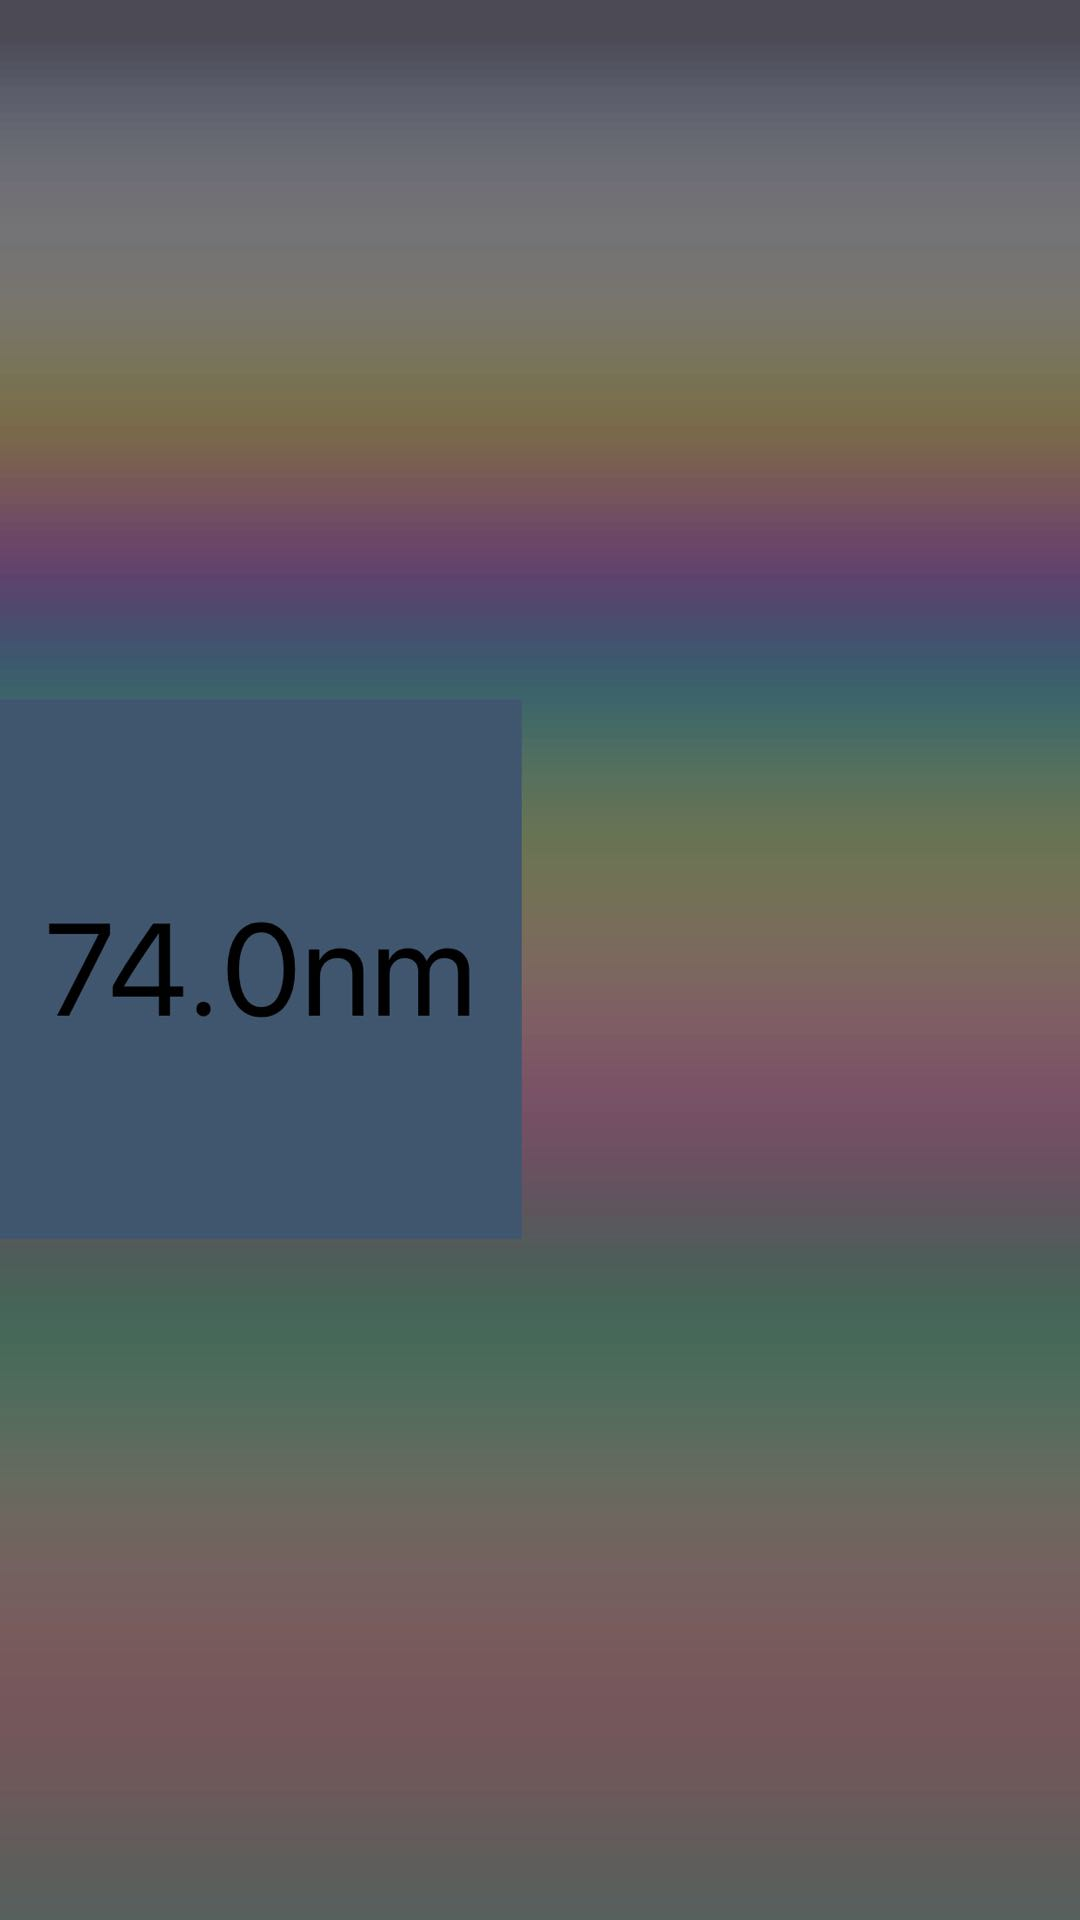
\includegraphics[width=0.9\textwidth]{../Pictures/color_app.jpeg}};
		\node[anchor = north,font=\bfseries] at (B.south) {软件界面};
		\only<2,3>{\fill [draw=none, fill=white, fill opacity=0.7] (B.north west) -- (B.north east) -- (B.south east) -- (B.south west) -- (B.north west) -- cycle;}
		\end{tikzpicture}	
	\end{column}
	\begin{column}[c]{0.65\textwidth}
		\begin{minipage}[c][0.8\textheight][c]{\linewidth}
			\begin{tikzpicture}
			\node[anchor=south west,inner sep=0] (B) at (0,0) {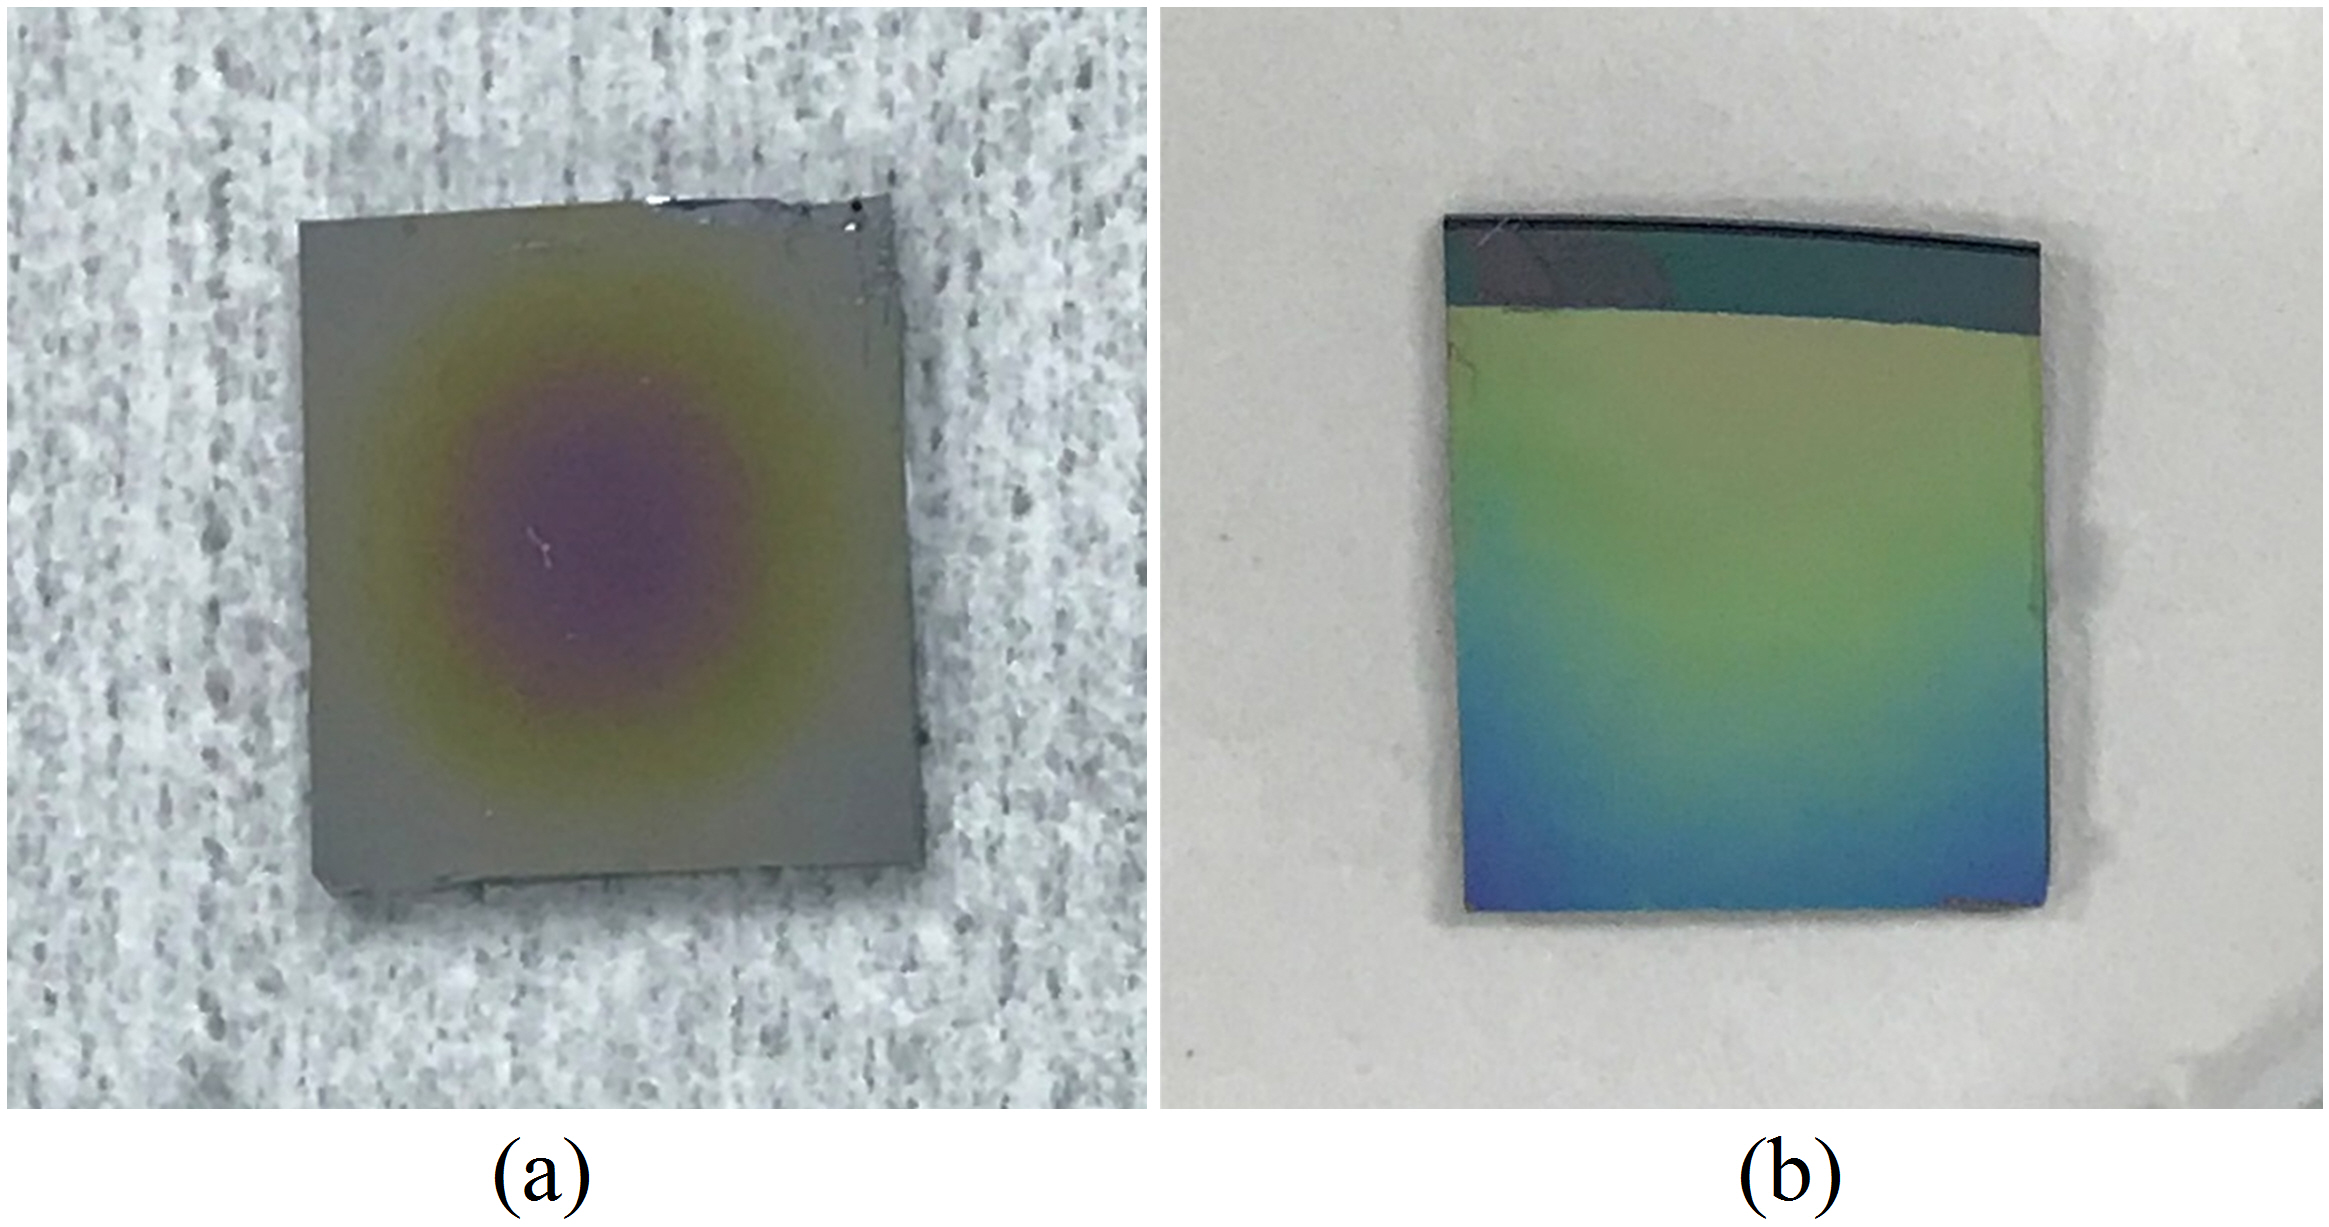
\includegraphics[width=\textwidth]{../Pictures/color_experiment.jpg}};
			\node[anchor = north,font=\bfseries,draw,red,xshift=-1.7cm] at (B.south) {中心厚度65~nm};
			\node[anchor = north,font=\bfseries,draw,red,xshift=1.7cm] at (B.south) {中心厚度90~nm};
			\only<2,3>{\fill [draw=none, fill=white, fill opacity=0.7] (B.north west) -- (B.north east) -- (B.south east) -- (B.south west) -- (B.north west) -- cycle;}
			\end{tikzpicture}	
		\end{minipage}
	\end{column}	
\end{columns}}
\only<2,3>{
	\centering
	\vspace{-7cm}
	\begin{tikzpicture}
		\node[anchor=south west,inner sep=0] (image) at (0,0) {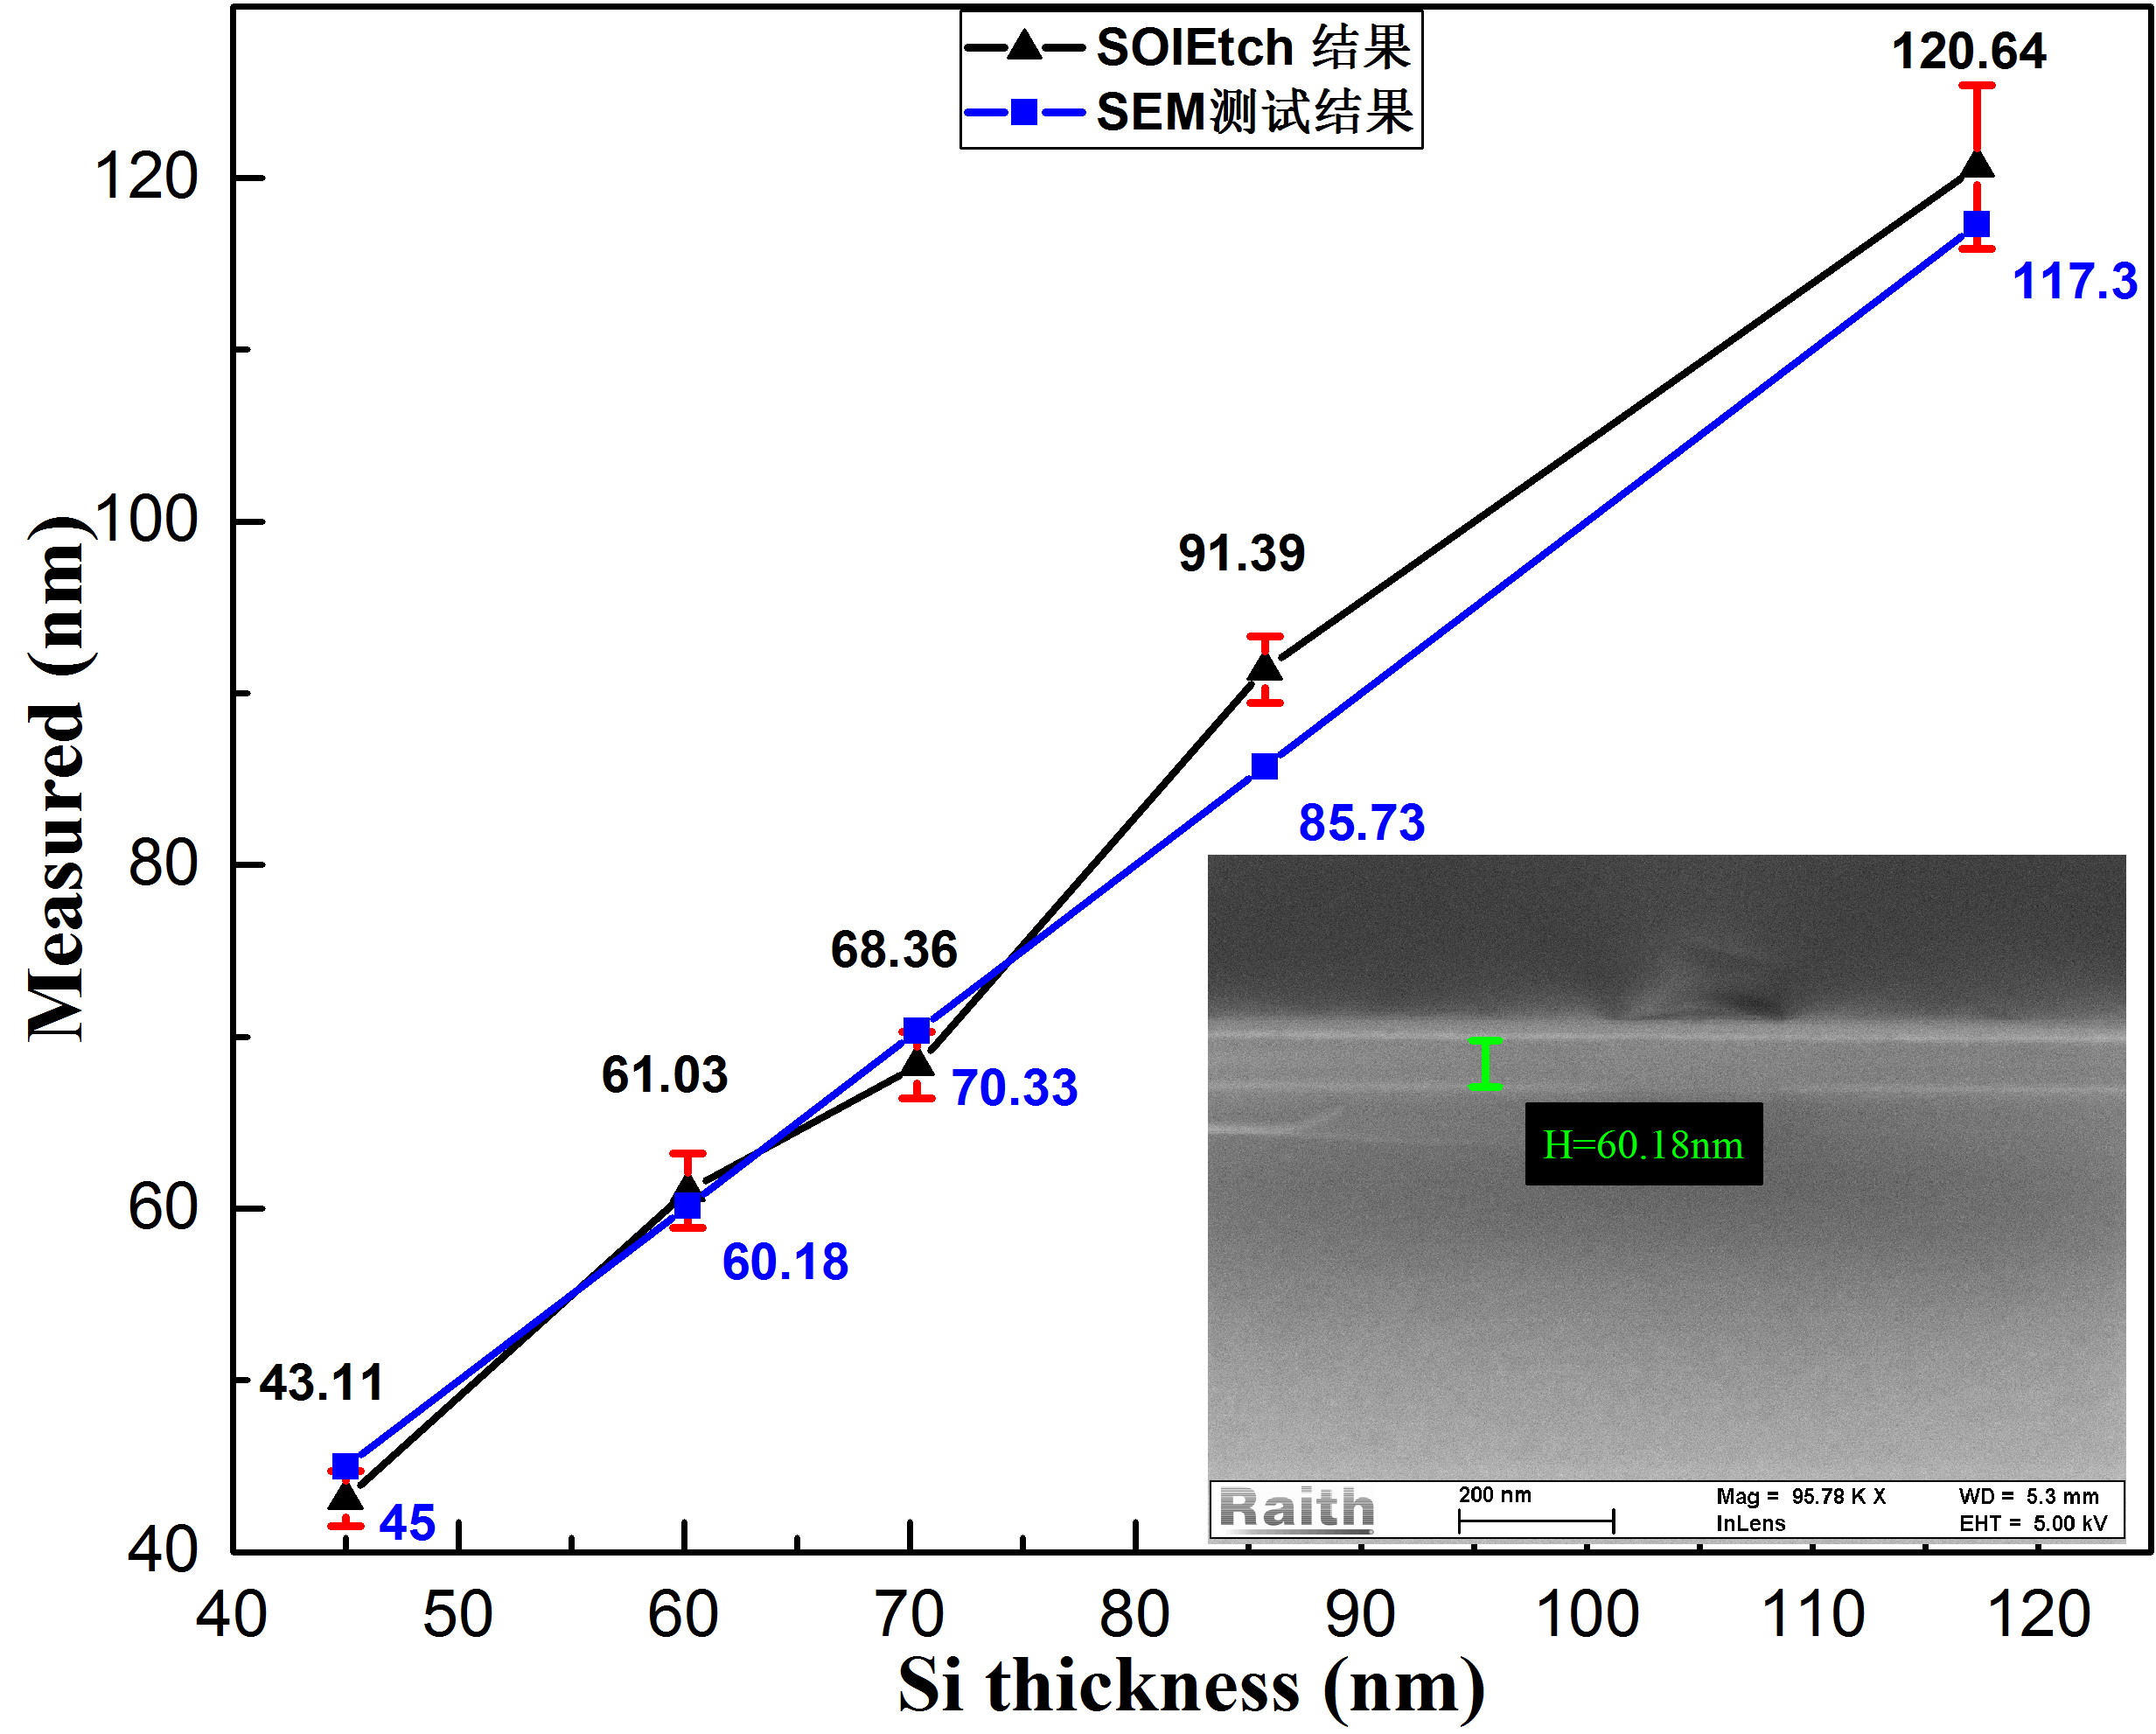
\includegraphics[width=0.7\textwidth]{../Pictures/color_experiment_measure.jpg}};
		\begin{scope}[x={(image.south east)},y={(image.north west)}]
		%\draw[help lines,xstep=.1,ystep=.1] (0,0) grid (1,1); %参考线绘制
			\only<3>{\node[anchor = center,red,draw,font=\bfseries] at (0.45,0.8) {平均值误差小于5.66~nm};}
		\end{scope}
	\end{tikzpicture}}
\end{frame}

\begin{frame}{颜色比较法测定硅层厚度}
\centering
\begin{tikzpicture}
	\node[anchor=south west,inner sep=0] (image) at (0,0) {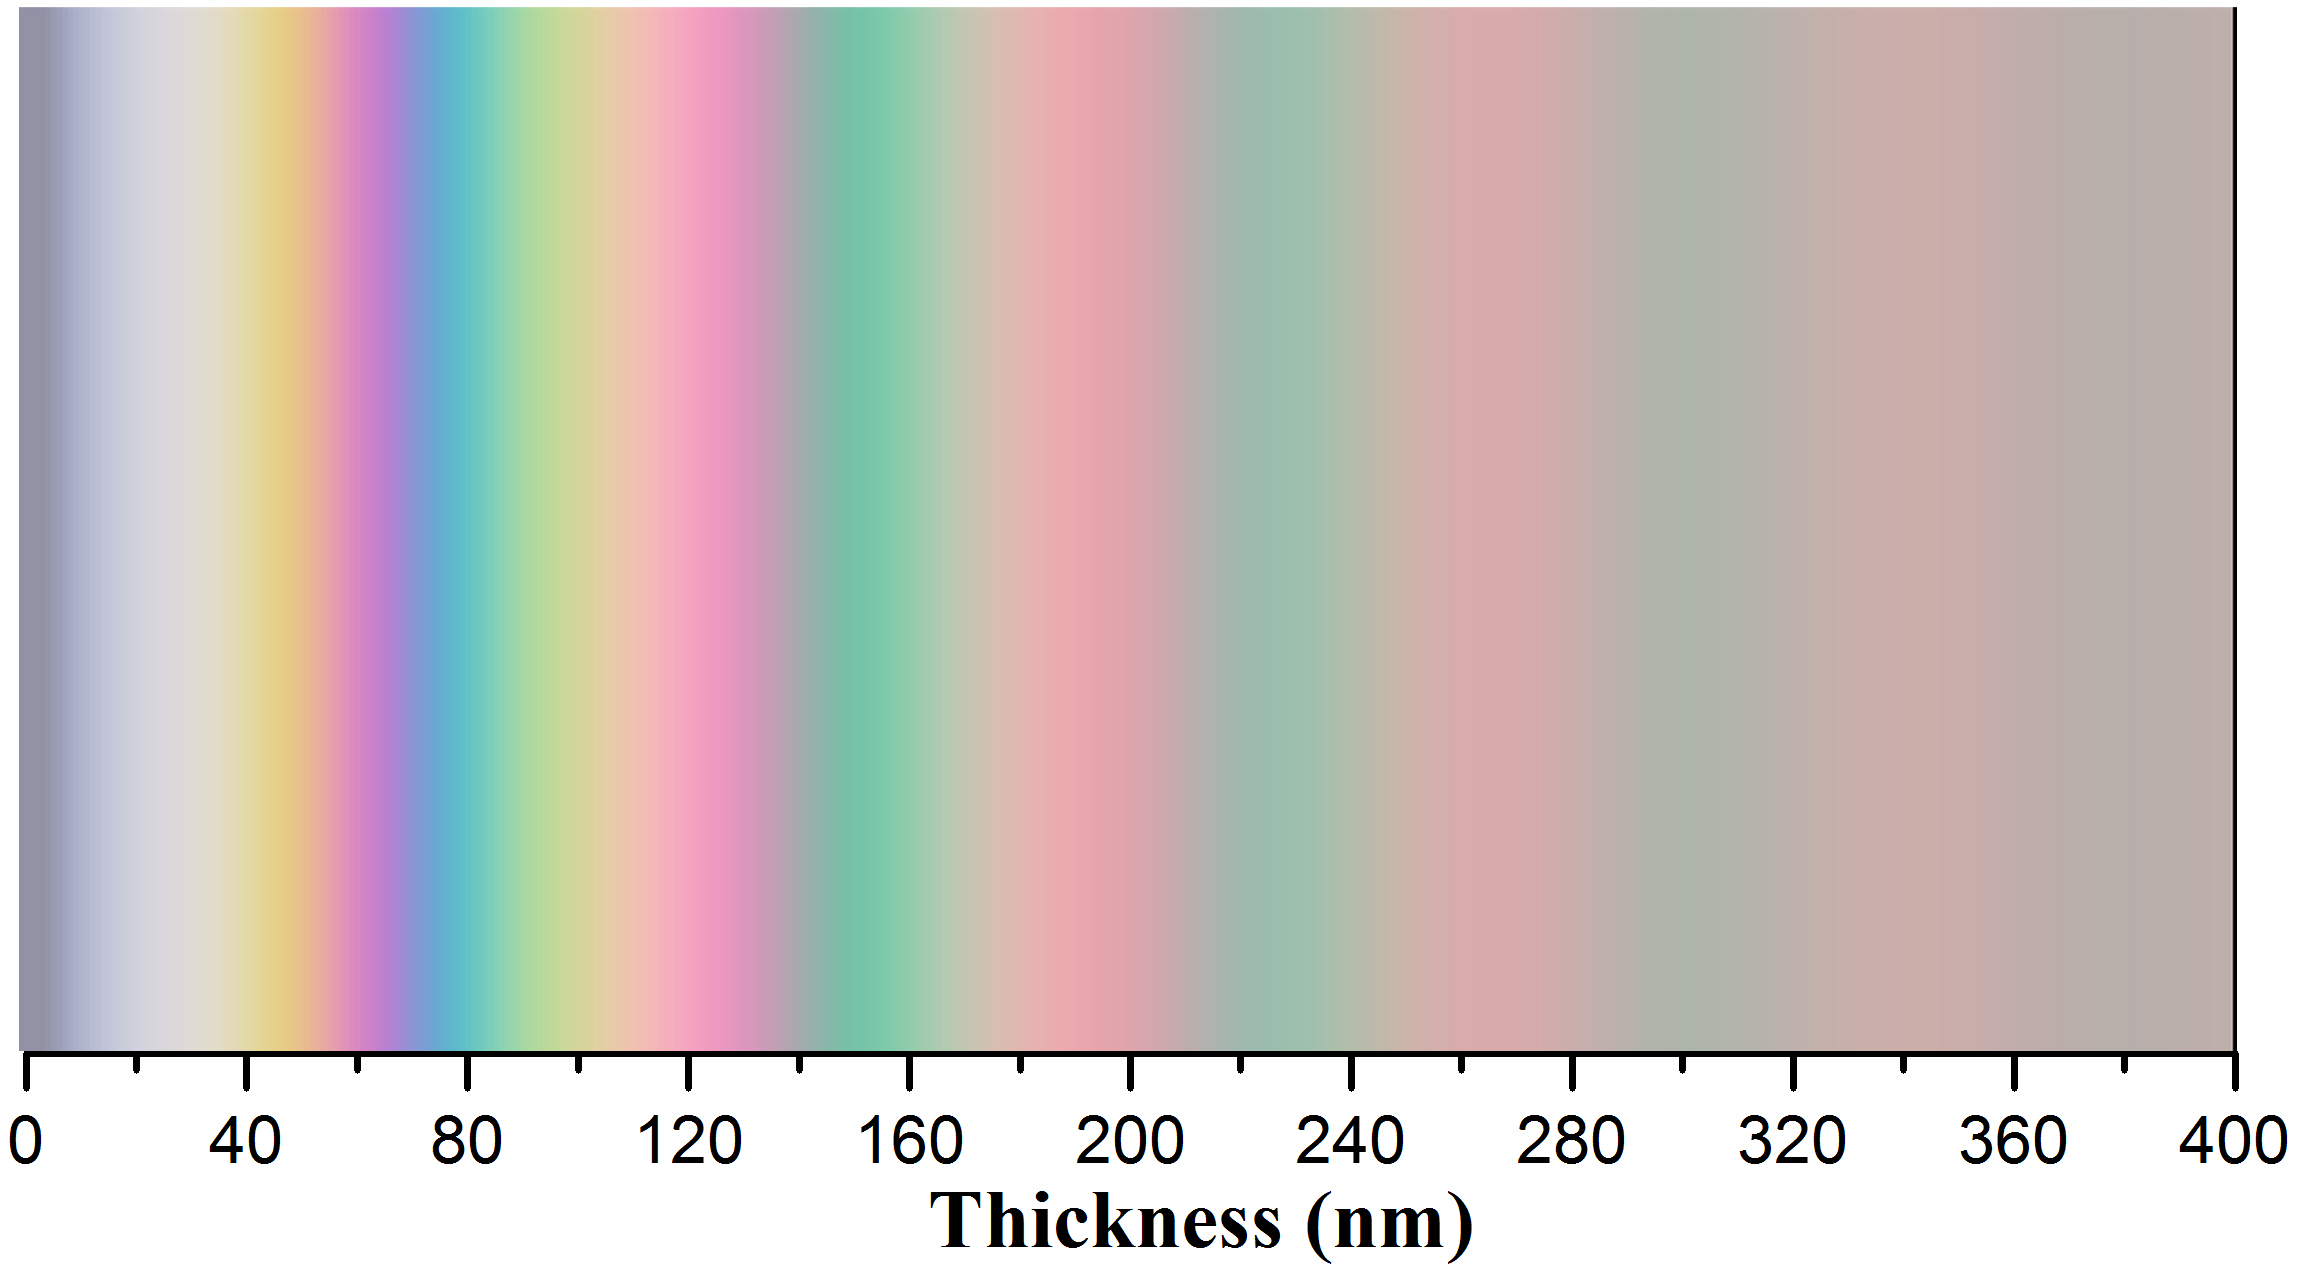
\includegraphics[width=0.8\textwidth]{../Pictures/color_400nm.jpg}};
	\begin{scope}[x={(image.south east)},y={(image.north west)}]
	%\draw[help lines,xstep=.1,ystep=.1] (0,0) grid (1,1); %参考线绘制
	\node[anchor = north,font=\bfseries] at (image.south) {0\~{}400~nm SOI芯片色谱图};
	\only<2>{
		\draw [ultra thick,line width=3mm,red,arrows=-{stealth},inner sep=4pt] (0.2,0.5) -- (0.8,0.5);
		\node[anchor = south,red,draw,font=\bfseries] at (0.5,0.62) {对比度逐渐降低};}
	\end{scope}
\end{tikzpicture}
\end{frame}

\begin{frame}{小结}
\zihao{4}
\begin{itemize}
	\item 提出了利用颜色比较的方法来测定\mbox{SOI}硅层\\厚度的方法
	\item 利用软件辅助,实现了当硅层厚度小于120~nm时,平均测量误差小于{\color{red}5.66~nm}
\end{itemize}
\end{frame}

\subsection{自脉冲\mbox{DFB}激光器及其应用}
\frame{\tableofcontents[currentsubsection]}
\begin{frame}{两段式自脉冲\mbox{DFB}激光器原理}	
\begin{columns}
		\begin{column}[c]{0.48\textwidth}
		\begin{minipage}[c][.3\textheight][c]{\linewidth}
			\begin{itemize}
				\item 色散自调Q开关(\mbox{dispersive self-Q-switching})
				\item 空间烧孔效应产生自脉冲
				\item 利用拍频产生自脉冲
			\end{itemize}
		\end{minipage}
	\end{column}	
	\begin{column}[c]{0.52\textwidth}
		\begin{tikzpicture}
		\node[anchor=south west,inner sep=0] (image) at (0,0) {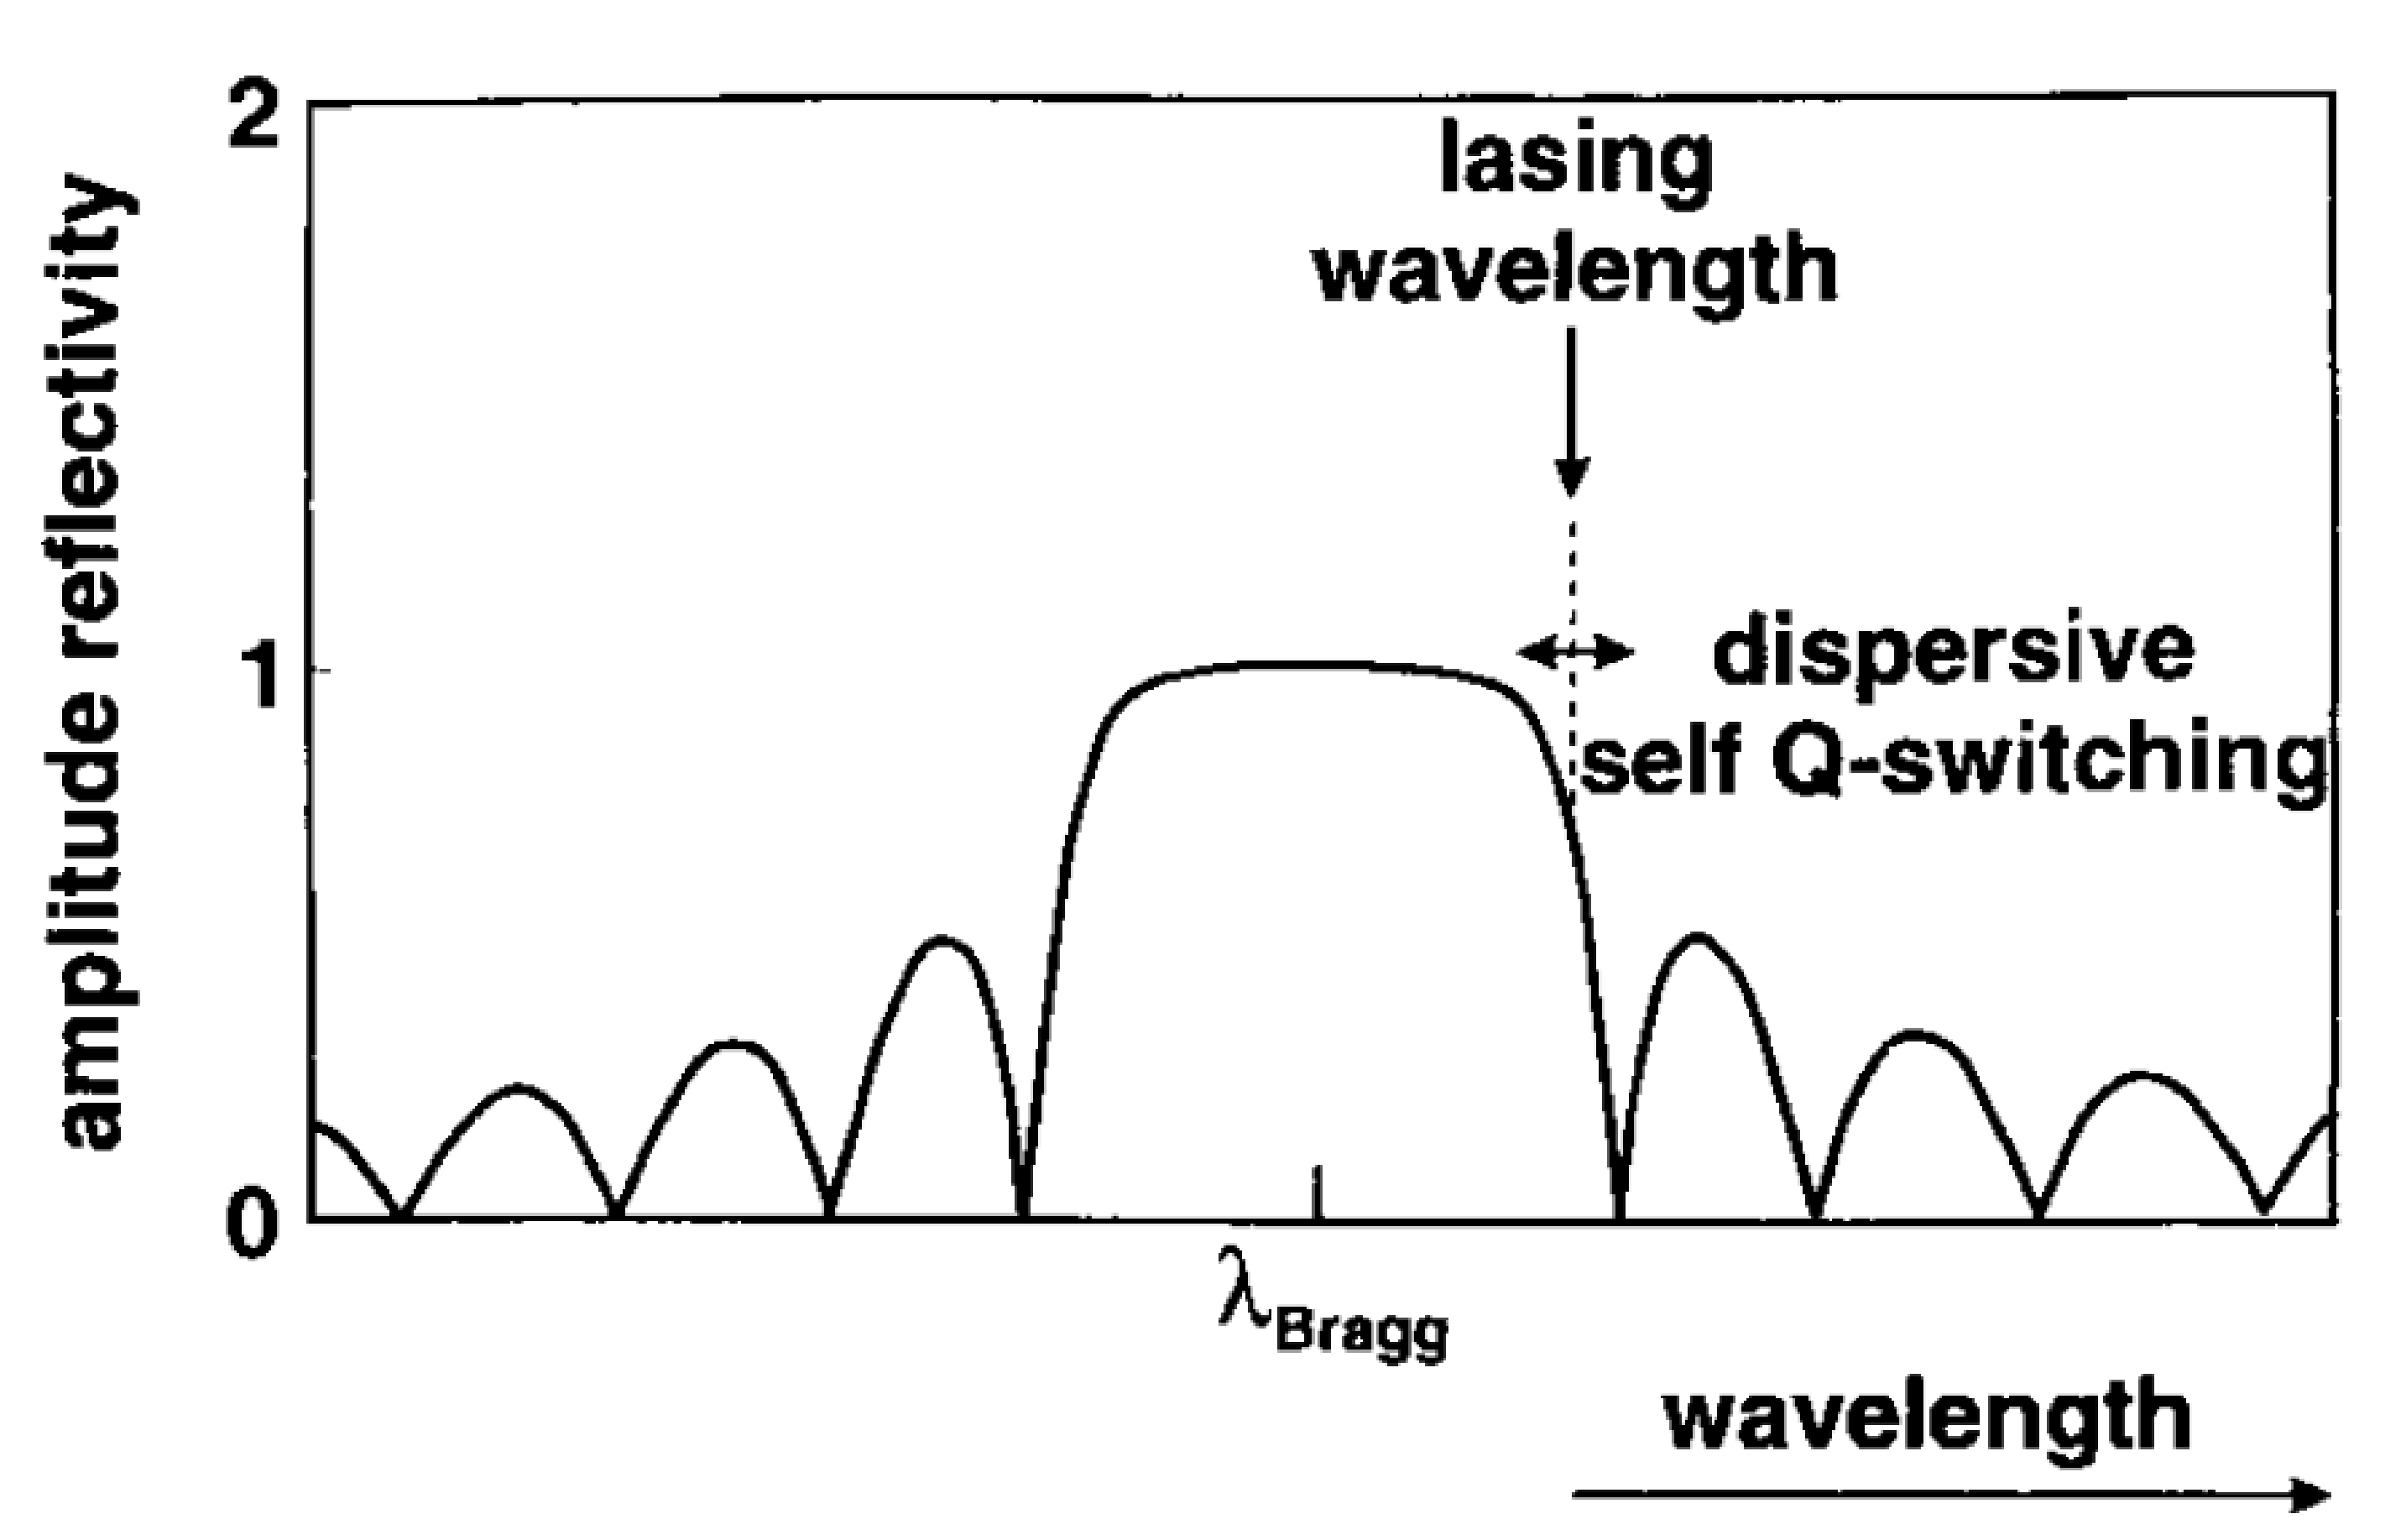
\includegraphics[width=0.95\textwidth]{../Pictures/laser_selfQswitching.jpg}};
		\node[anchor=south,inner sep=4pt]  at (image.north) {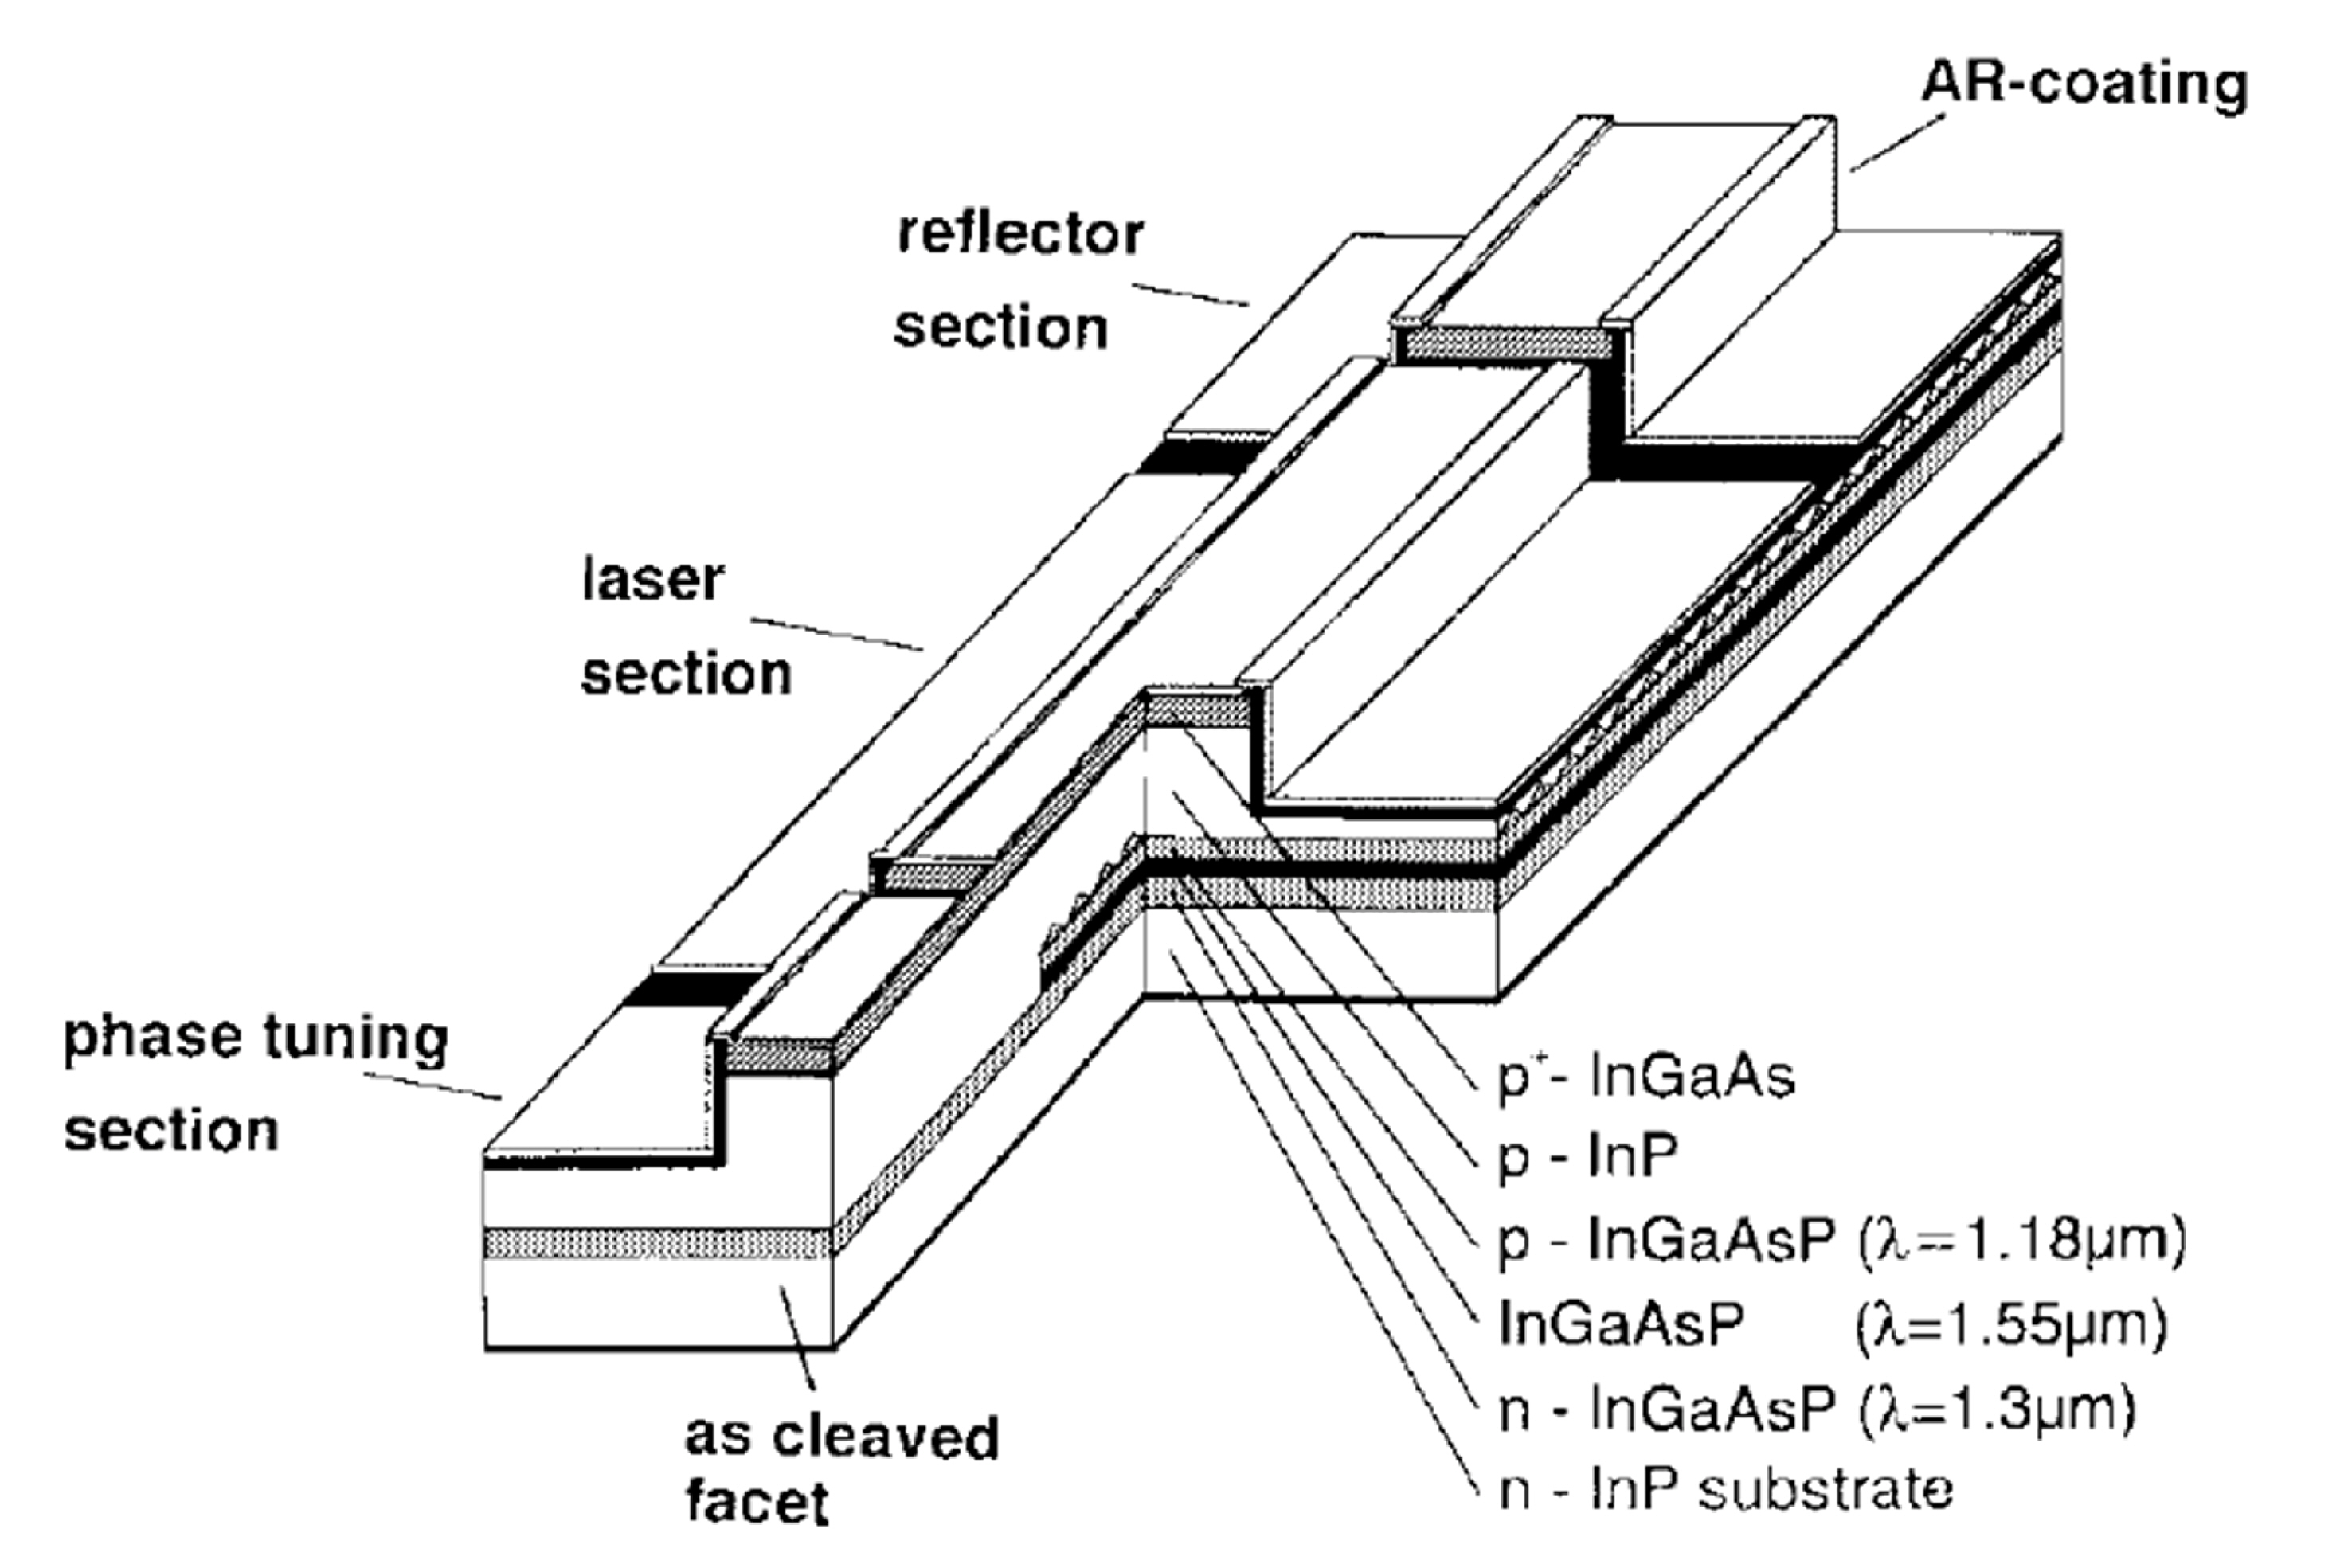
\includegraphics[width=0.95\textwidth]{../Pictures/laser_twosectiondfb.jpg}};
		\node[anchor = south east,inner sep=0] at (image.north east) {\bfseries\tiny \emph{Mohrle M., Photon. Technol. Lett. 4(9)}};
			\begin{scope}[x={(image.south east)},y={(image.north west)}]
				%\draw[help lines,xstep=.1,ystep=.1] (0,0) grid (1,1); %参考线绘制
				 \draw<1,3> [ultra thick,red,arrows=-{stealth}] (0.66,0.2) -- (0.66,0.53);
				 \draw<2> [ultra thick,red,arrows=-{stealth}] (0.72,0.2) -- (0.72,0.53);
			\end{scope}
		\end{tikzpicture}	
	\end{column}
\end{columns}
\end{frame}

\begin{frame}{硅基III-V混合集成技术}
\centering
\begin{tikzpicture}
\node[anchor=south west,inner sep=0] (image) at (0,0) {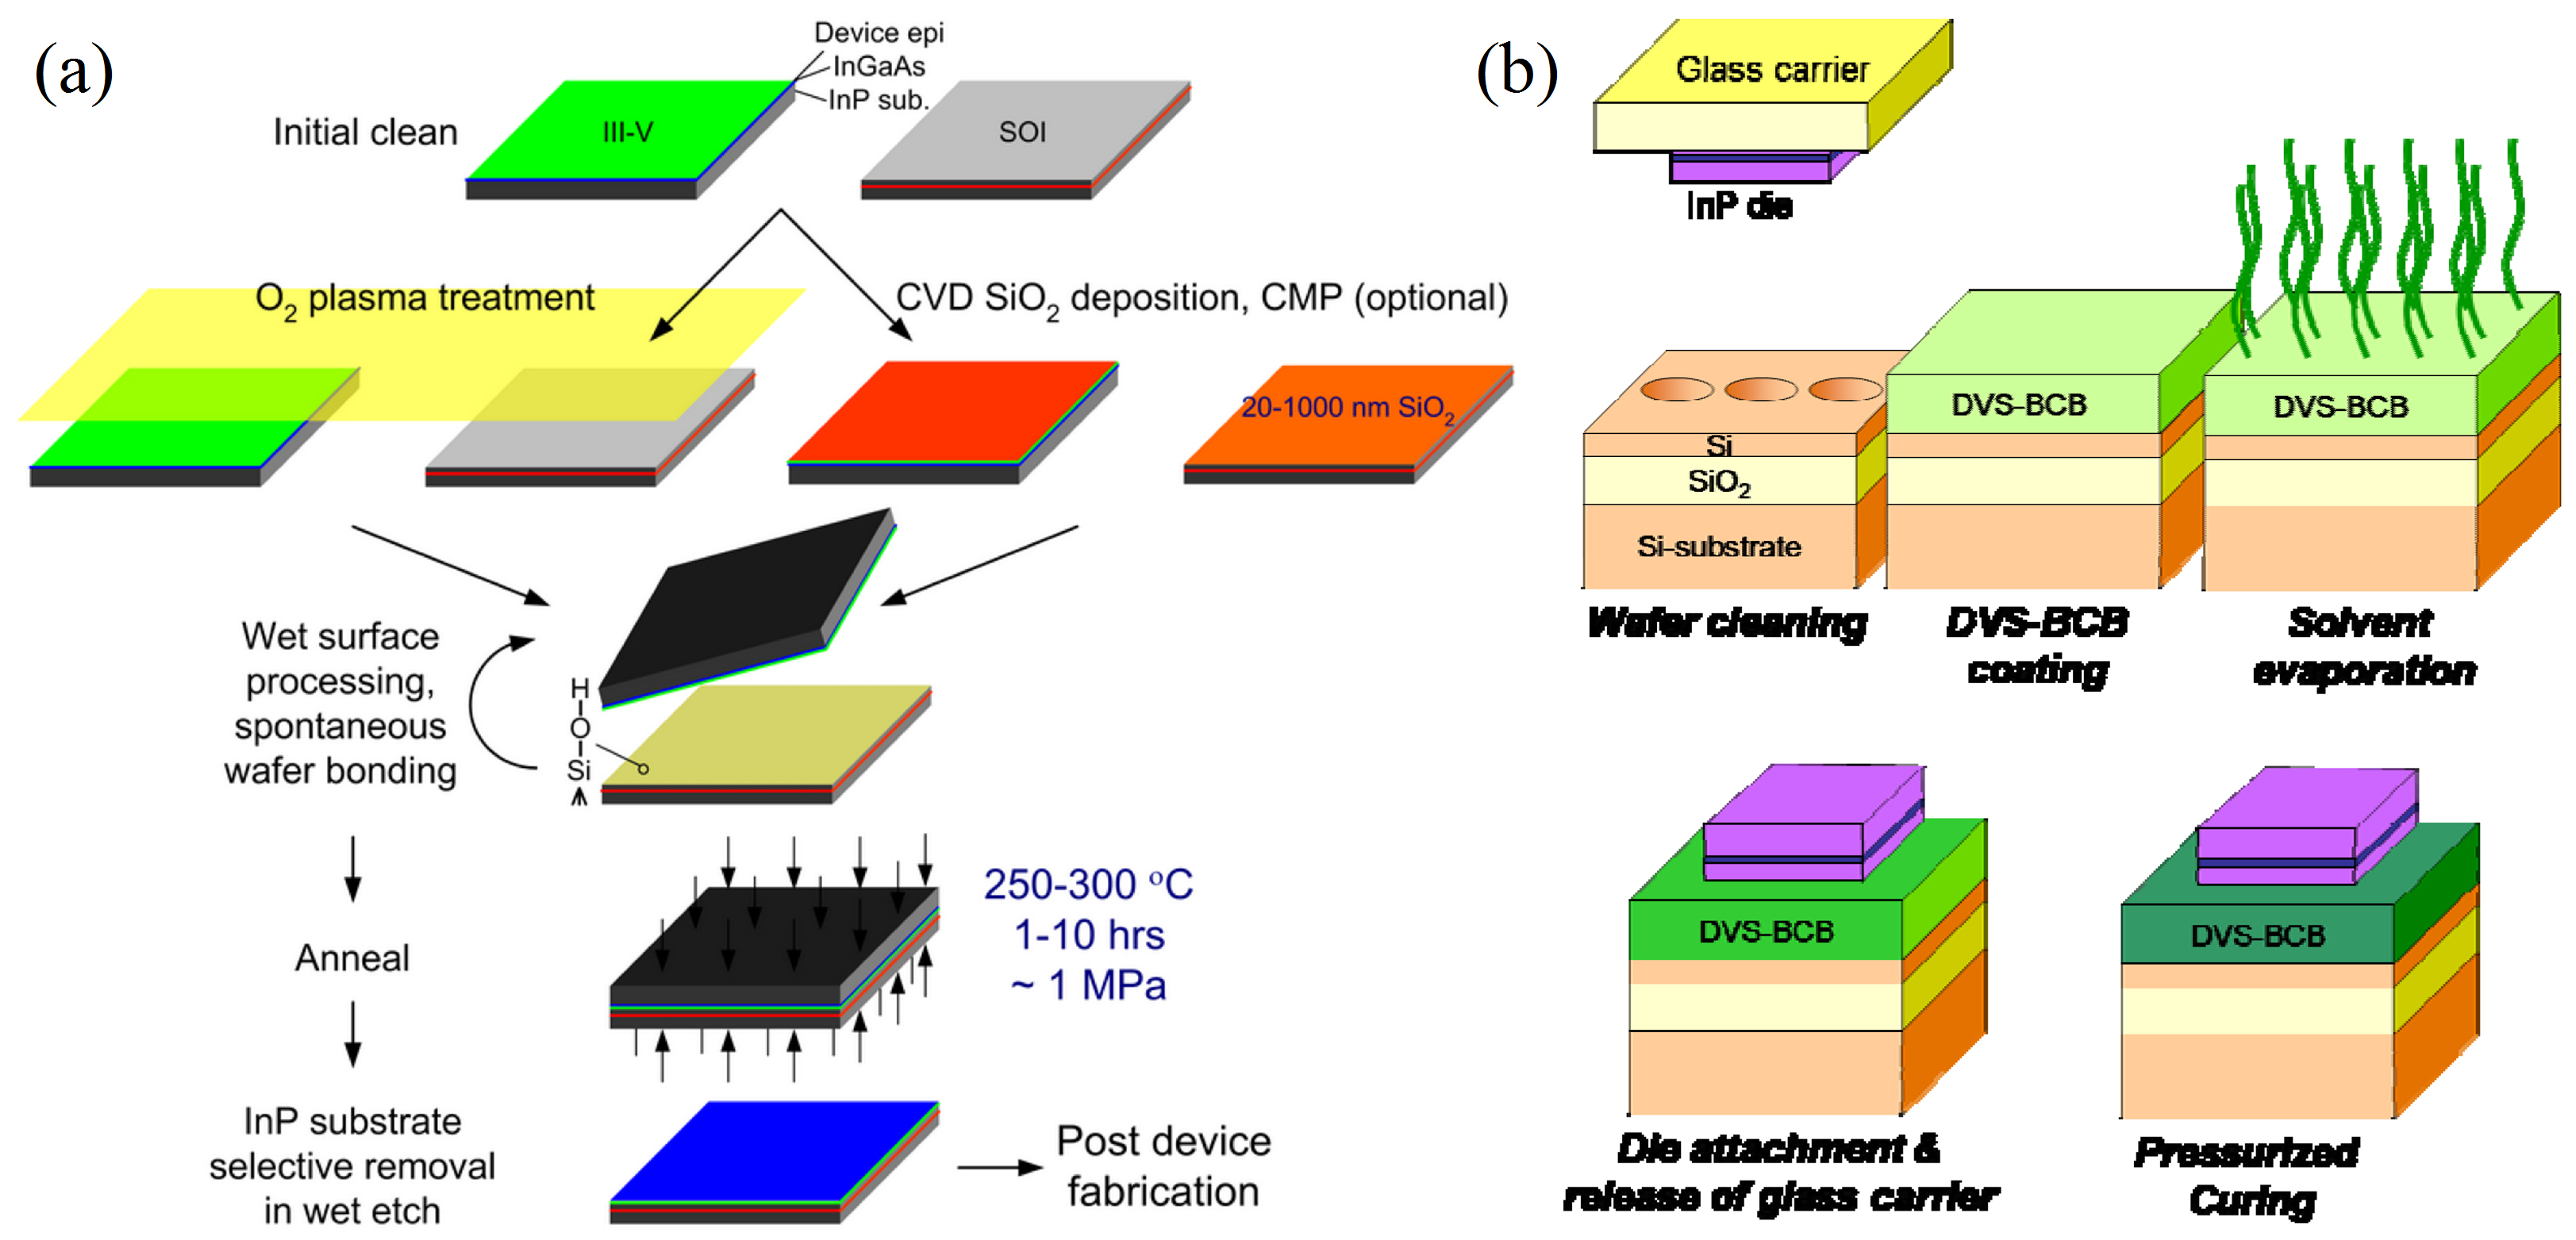
\includegraphics[width=\textwidth]{../Pictures/laser_bonding.jpg}};
	\begin{scope}[x={(image.south east)},y={(image.north west)}]
	%\draw[help lines,xstep=.1,ystep=.1] (0,0) grid (1,1); %参考线绘制
	\node[anchor = north,inner sep=4pt,font=\bfseries] at (0.25,0) {共价键键合};
	\node[anchor = north,inner sep=4pt,font=\bfseries] at (0.75,0) {胶键合};
	\end{scope}
\end{tikzpicture}
\end{frame}

\begin{frame}{器件的设计}
\uncover<1>
{
\centering{\mbox{III-V}外延片的材料参数}
\begin{table}[h]
	\centering
	\zihao{6}
	\begin{tabular}[t]{|llll|}
		\hline
		\textbf{名称} & \textbf{材料组分} & \textbf{掺杂浓度 ($\pmb{cm^{-3}}$)} & \textbf{厚度($\pmb{nm}$)} \\
		\hline
		Sacrificial & InP & - &  200 \\
		\hline 
		Sacrificial & InGaAs & - &  200 \\
		\hline
		N cladding & InP & 1.00E18 & 190 \\
		\hline
		SCH & InGaAsP(Q1.17) & - & 100 \\
		\hline
		MQW well$\times$6 & InGaAsP(Q1.55) & - & 7 \\
		\hline
		MQW barrier$\times$7 & InGaAsP(Q1.17) & - & 9 \\
		\hline
		SCH & InGaAsP(Q1.17) & - & 100 \\
		\hline
		P cladding & InP & 5.00E17 & 500 \\
		\hline 
		P cladding & InP & 5.00E17->2.00E18 & 1000\\
		\hline
		Transition & InGaAsP(Q1.2) & >3.00E18 & 10\\
		\hline
		Transition & InGaAsP(Q1.4) & >3.00E18 & 10\\
		\hline
		P contact & InGaAsP & >1.5E19 & 200 \\
		\hline
		Sacrificial & InP & - & 200 \\
		\hline
		Stop etch & InGaAs & - & 200 \\
		\hline
		Substrate & InP & - & -\\
		\hline
	\end{tabular}
\end{table}}

\only<2>{
	\vspace{-6.5cm}
	\centering
\begin{tikzpicture}
	\node[anchor=south west,inner sep=0] (image) at (0,0) {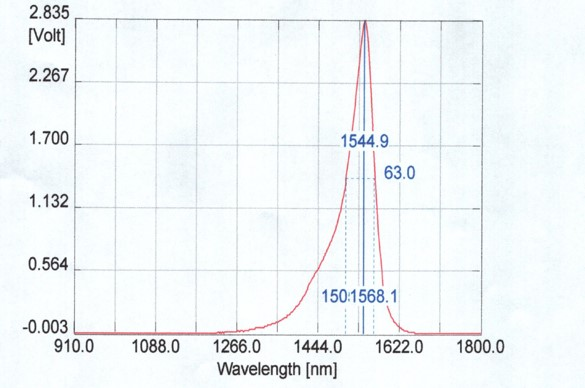
\includegraphics[width=0.9\textwidth]{../Pictures/laser_PL.jpg}};
	\node[anchor = north,red,draw,inner sep=4pt,font=\bfseries,yshift=2cm] at (image.center) {PL谱};
\end{tikzpicture}}
\end{frame}

\begin{frame}{器件的设计}
\centering
	\begin{tikzpicture}
	\node[anchor=south west,inner sep=0] (image) at (0,0) {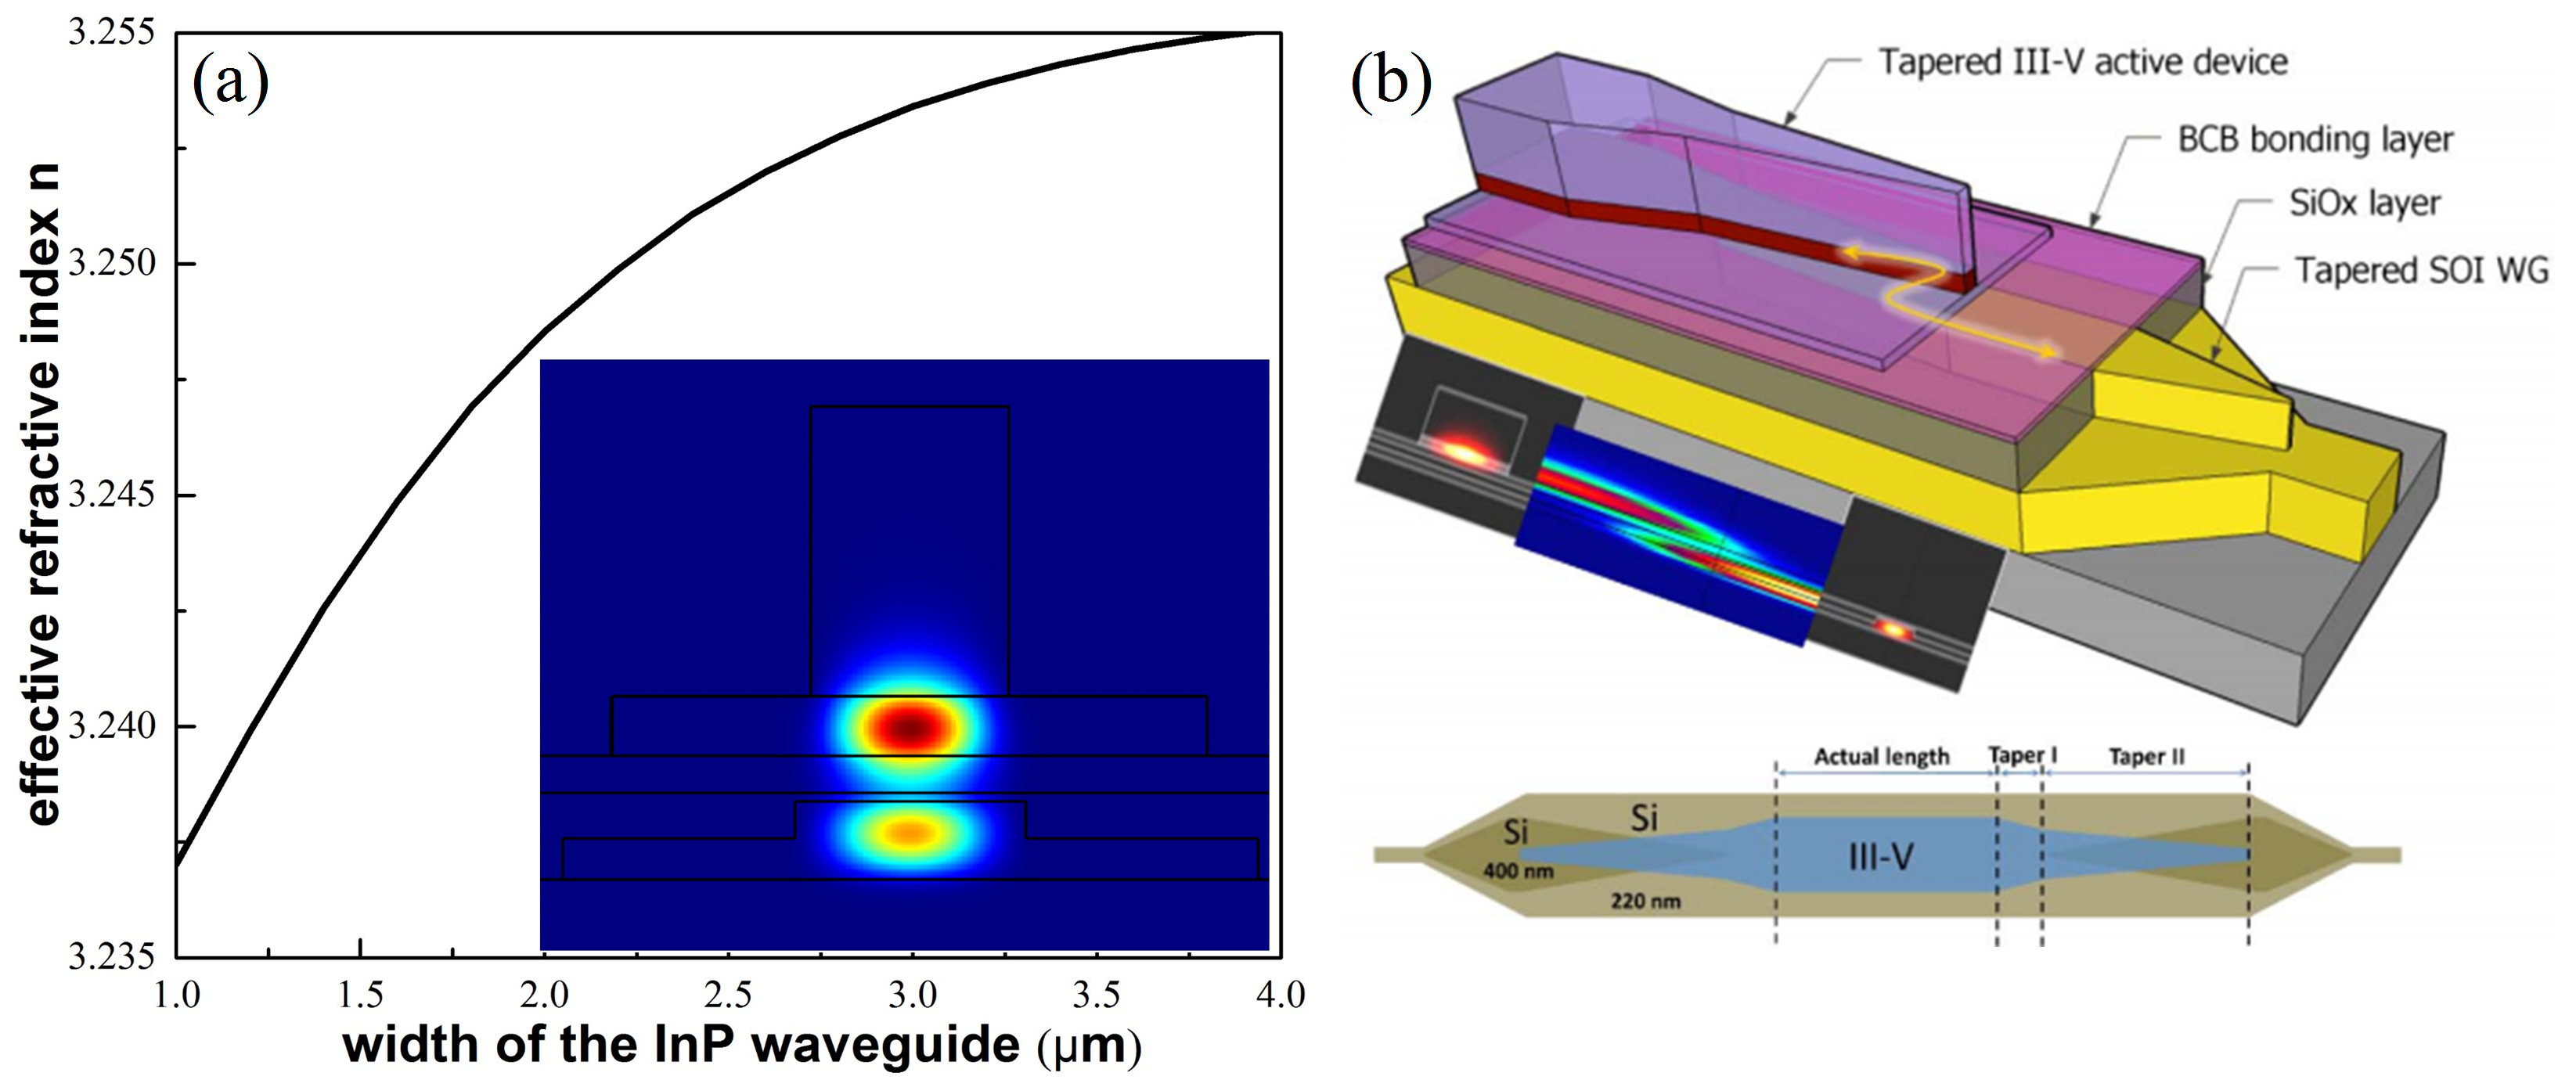
\includegraphics[width=\textwidth]{../Pictures/laser_modeandtaper.jpg}};
	\begin{scope}[x={(image.south east)},y={(image.north west)}]
		%\draw[help lines,xstep=.1,ystep=.1] (0,0) grid (1,1); %参考线绘制
		\node[anchor = east] at (1,0.1) {\bfseries\tiny \emph{Keyvaninia S., Opt. Lett., 38(24)}};
	\onslide+<2,3>{
		\node[anchor = north,red,inner sep=4pt,font=\bfseries](formula) at (image.south) {$2\Delta n_{eff}\Lambda = \Delta\lambda$};
		\node[anchor = north,red,draw,inner sep=4pt,font=\bfseries](formula1) at (formula.south) {$\Delta\lambda\approx 4 nm, \Delta n_{eff}\approx 0.009$};
		\draw[red,ultra thick] (0.5,0.12) -- (0.5,0.97) --(0.07,0.97);
		\draw[red,ultra thick] (0.21,0.12) -- (0.21,0.68) --(0.07,0.68);}
	\only<3>{\node[anchor = center,red,inner sep=4pt,font=\bfseries](formula) at (0.9,0.4) {Taper};}
	\end{scope}
	\end{tikzpicture}
\end{frame}

\begin{frame}{激光器的结构}
\centering
\begin{tikzpicture}
\node[anchor=south west,inner sep=0] (image) at (0,0) {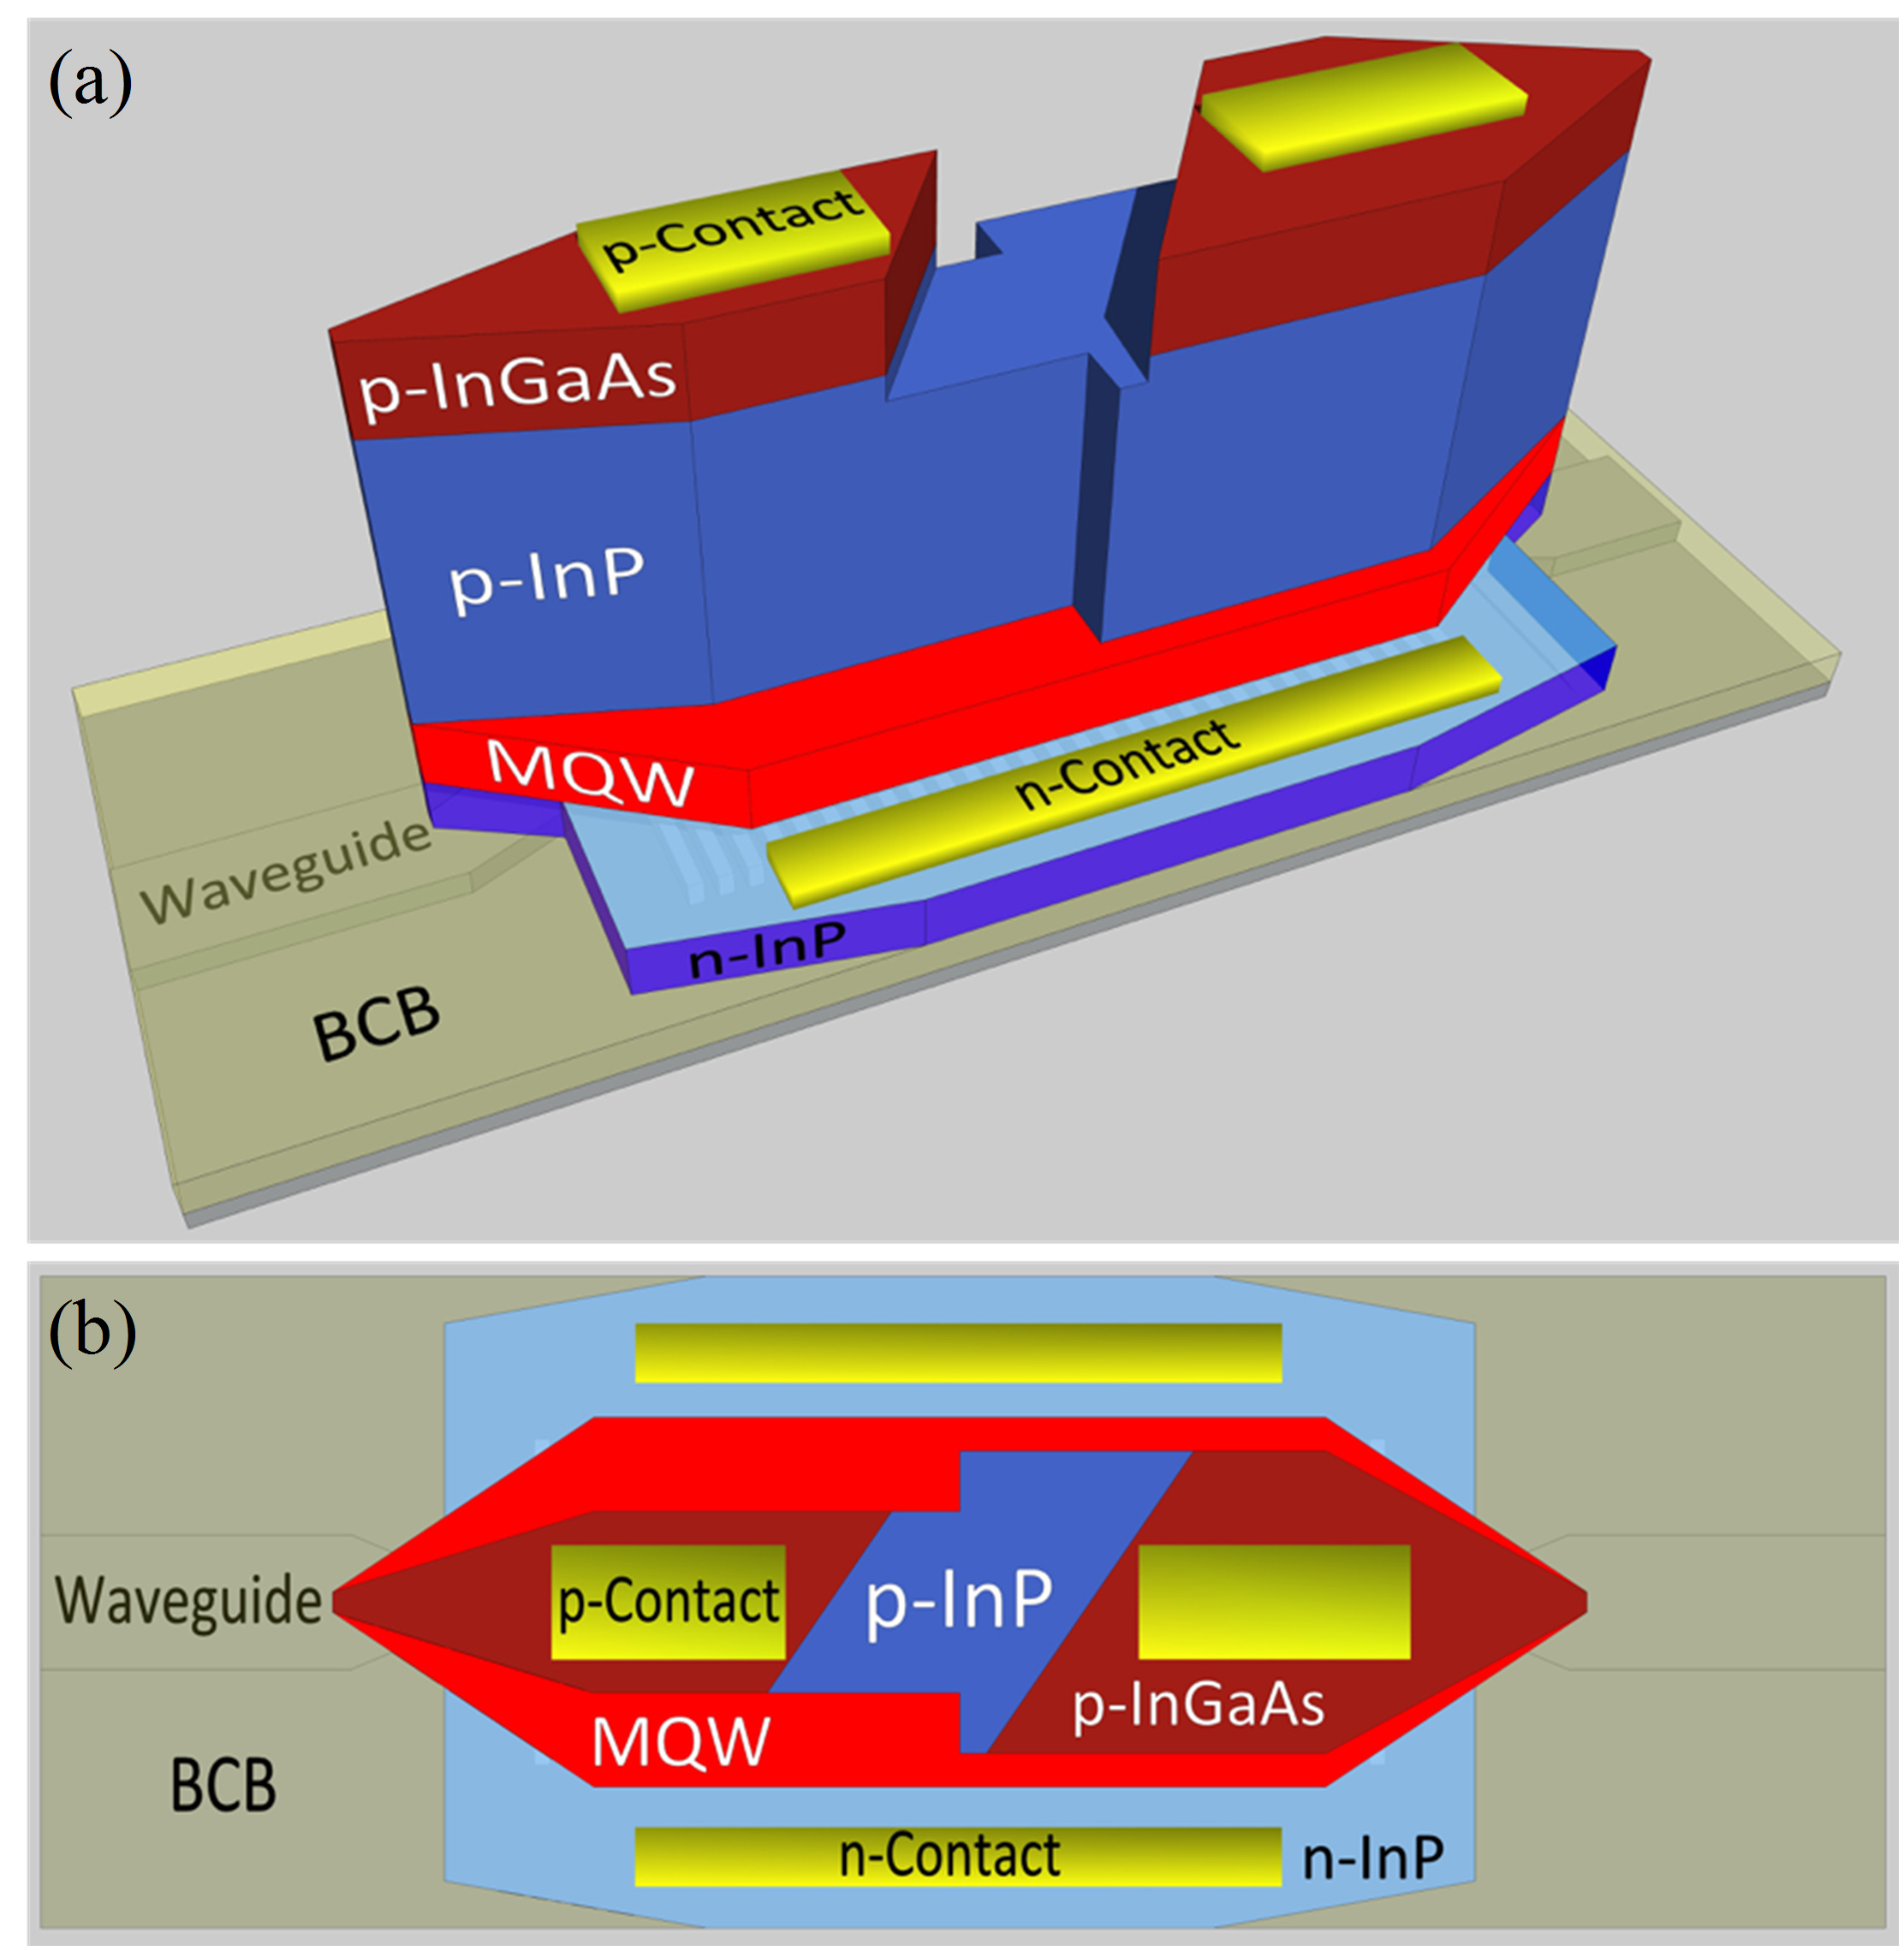
\includegraphics[width=0.6\textwidth]{../Pictures/laser_structure.jpg}};
\begin{scope}[x={(image.south east)},y={(image.north west)}]
%\draw[help lines,xstep=.1,ystep=.1] (0,0) grid (1,1); %参考线绘制
\end{scope}
\end{tikzpicture}
\end{frame}

\begin{frame}{器件的制作}
\centering
\begin{tikzpicture}
\node[anchor=south west,inner sep=0] (image) at (0,0) {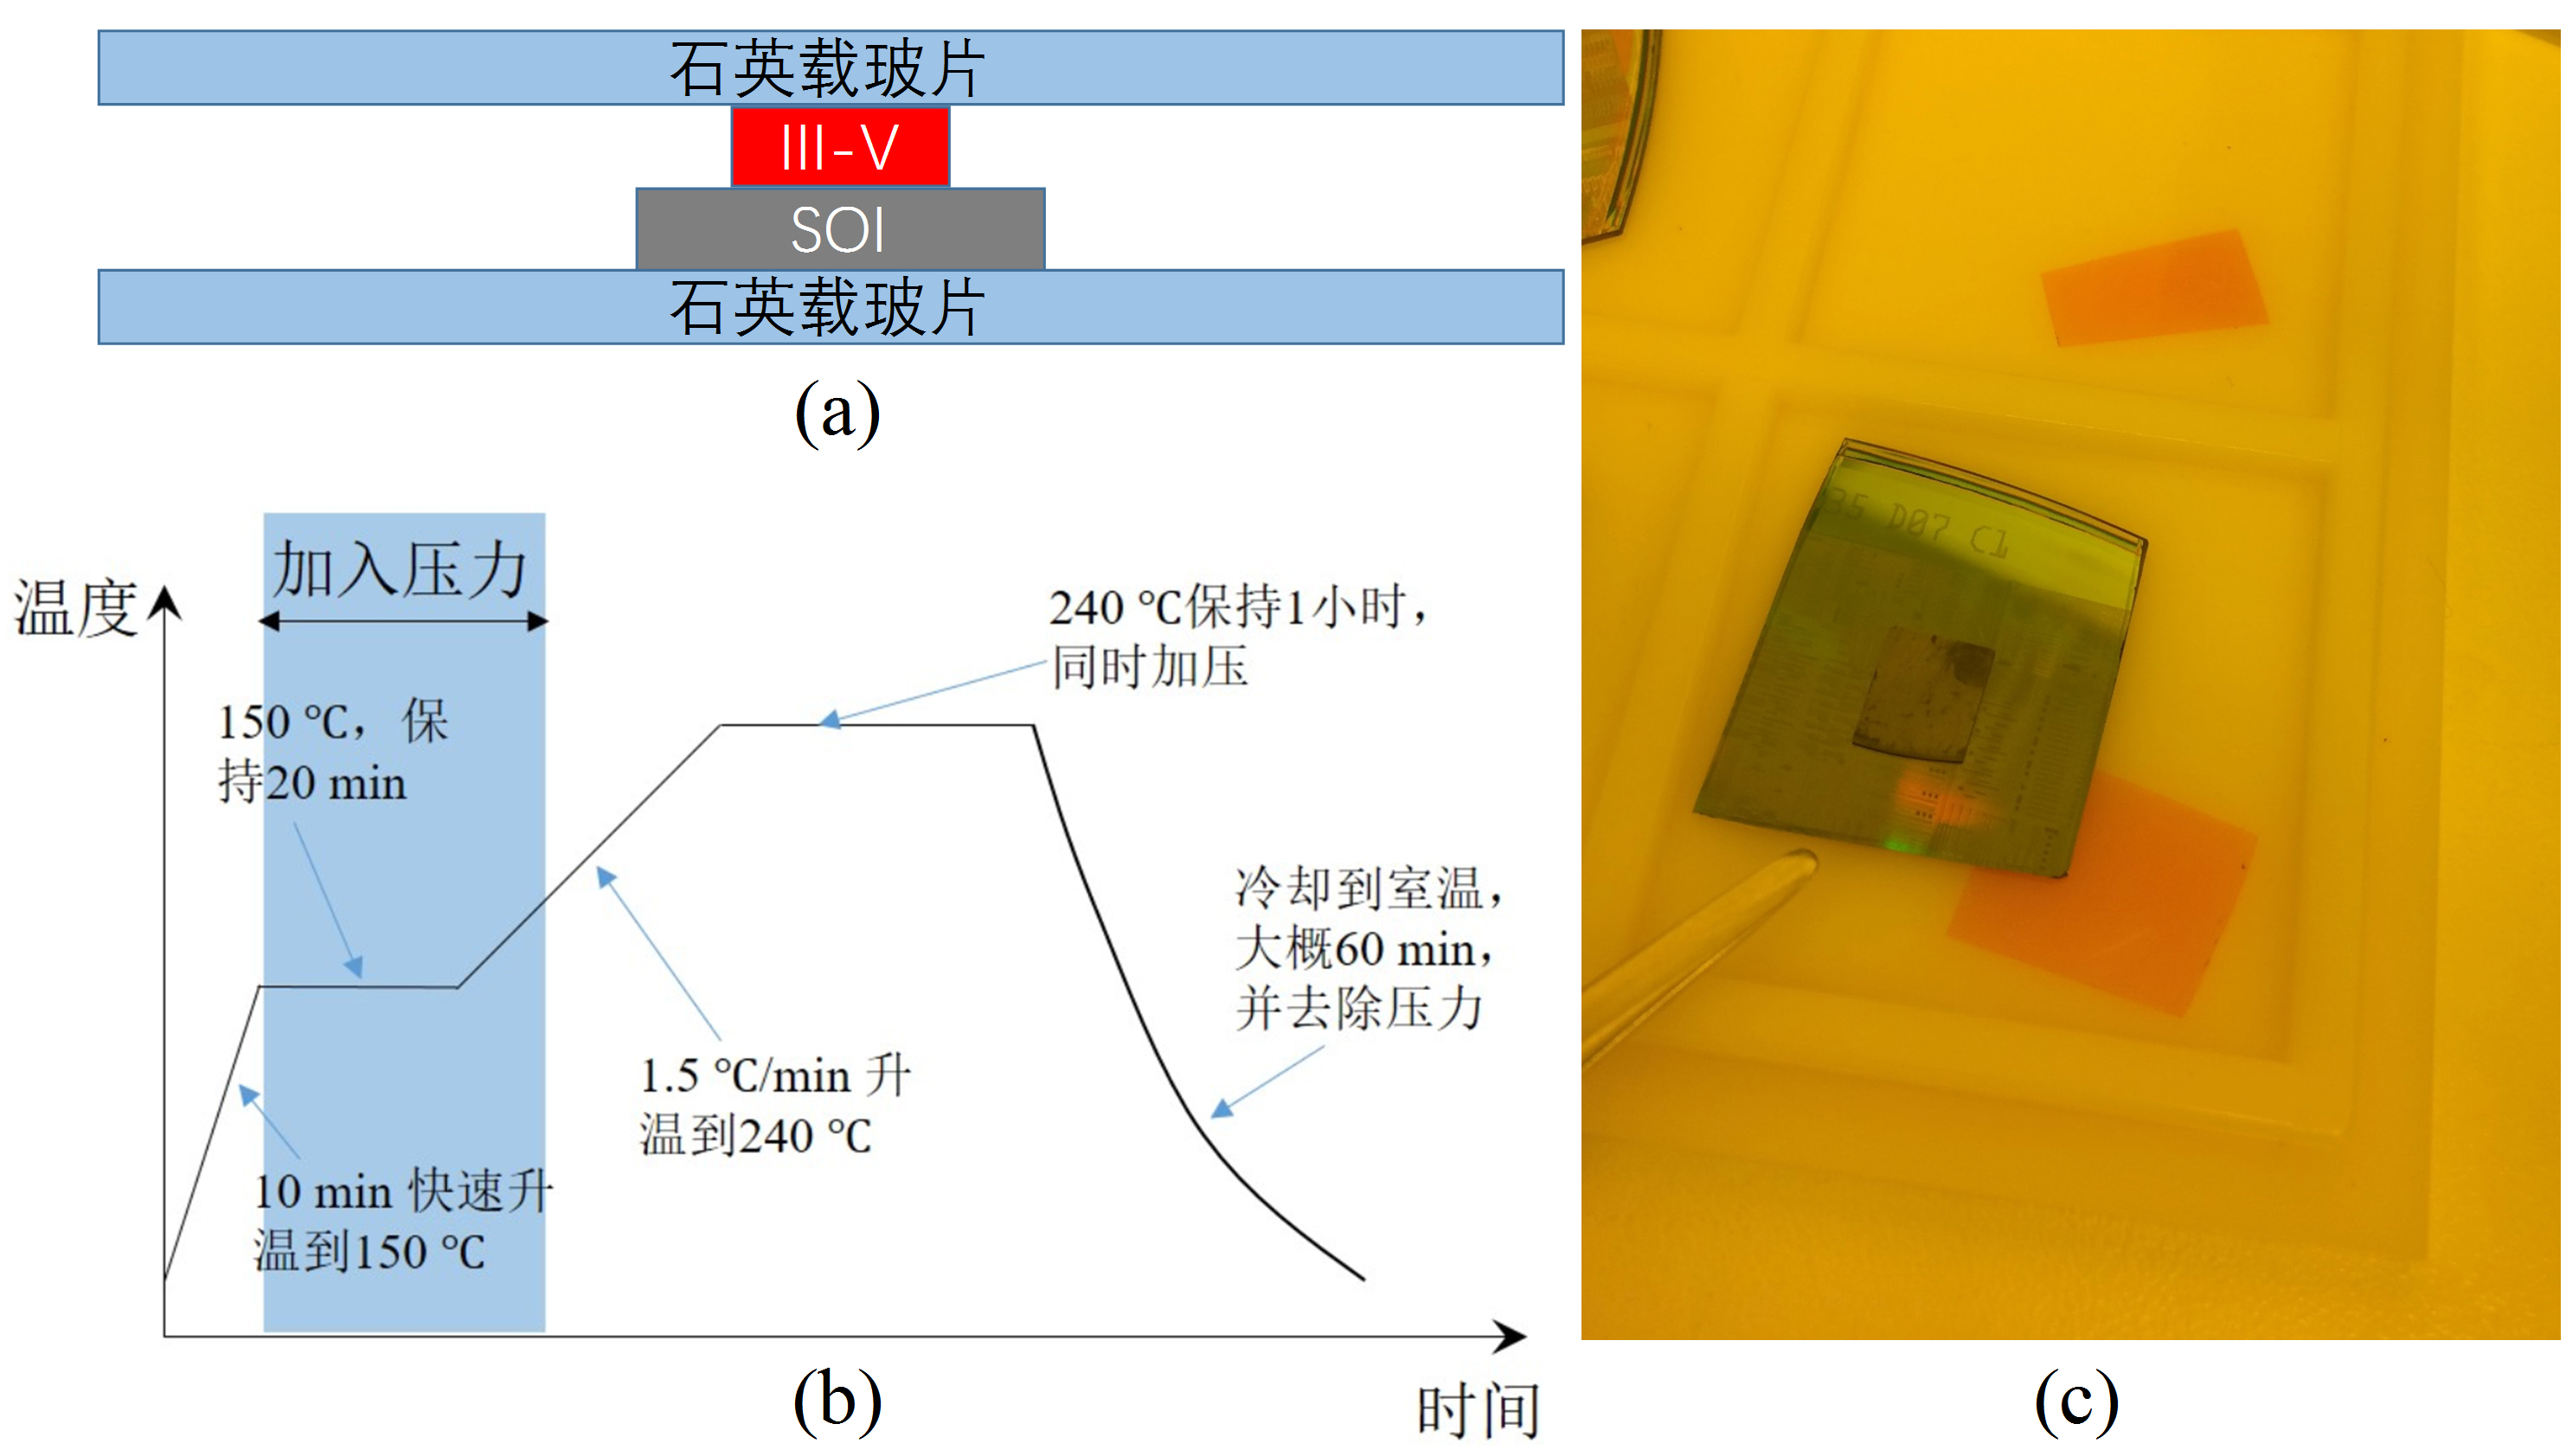
\includegraphics[width=\textwidth]{../Pictures/laser_bonder.jpg}};
\begin{scope}[x={(image.south east)},y={(image.north west)}]
%\draw[help lines,xstep=.1,ystep=.1] (0,0) grid (1,1); %参考线绘制
\end{scope}
\end{tikzpicture}
\end{frame}

\begin{frame}{器件的制作}
\centering
\begin{tikzpicture}
\node[anchor=south west,inner sep=0] (image) at (0,0) {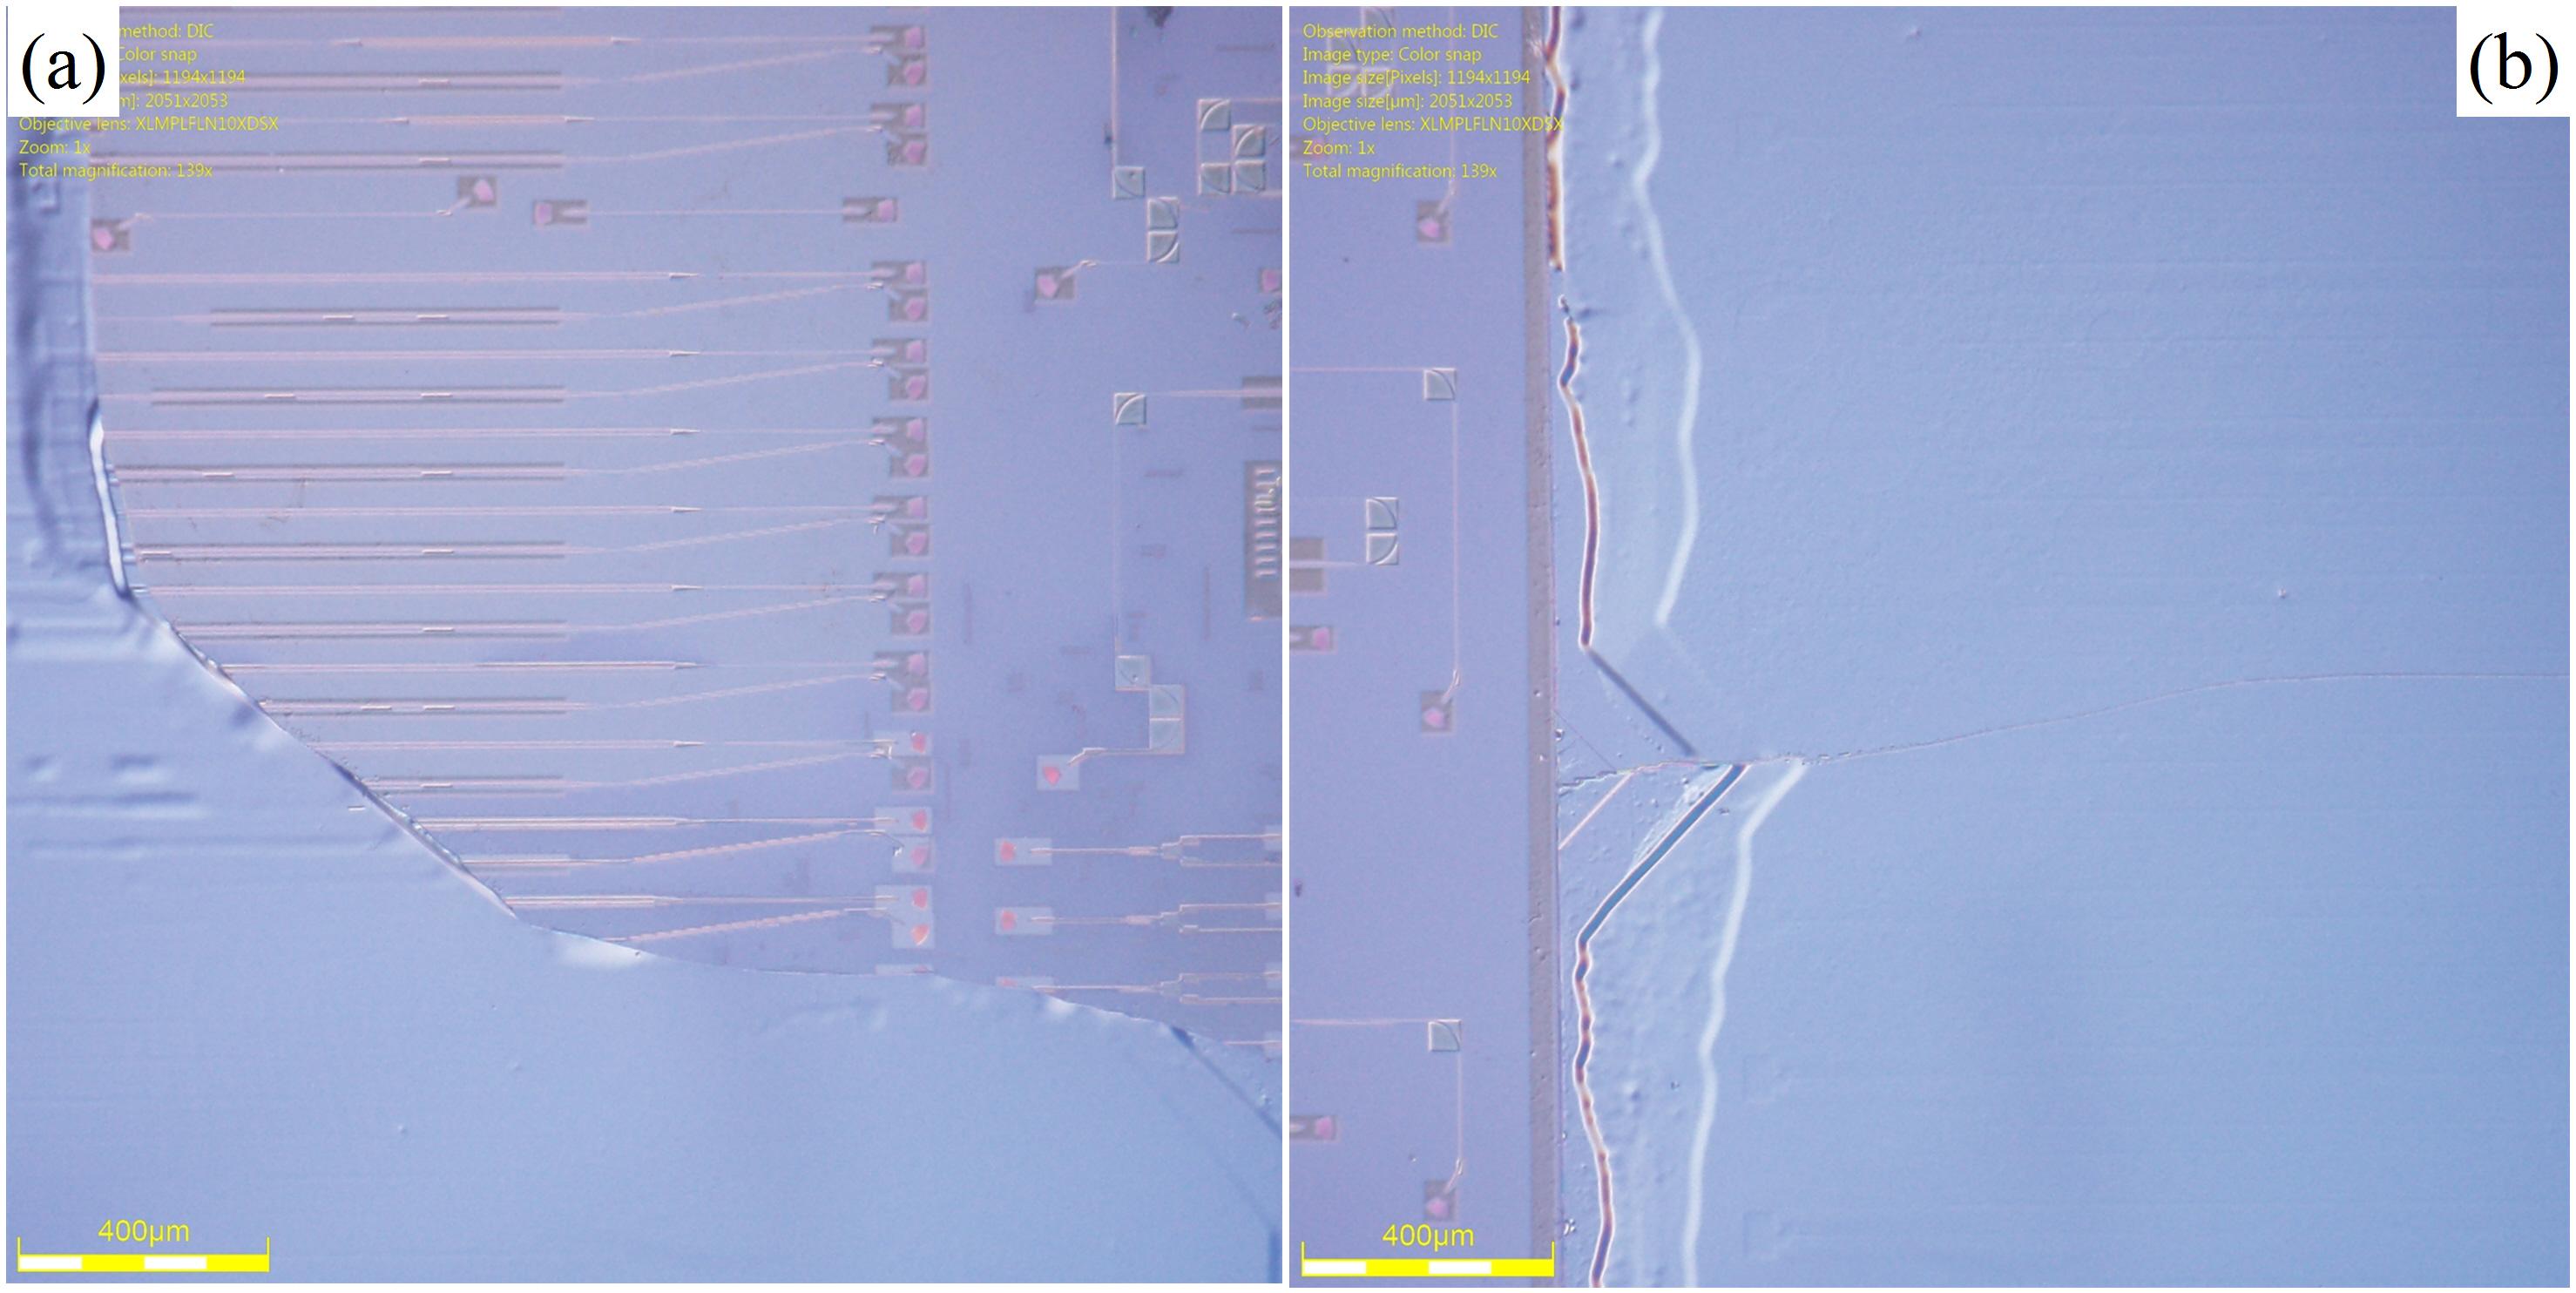
\includegraphics[width=\textwidth]{../Pictures/laser_sub_removal.jpg}};
\node[anchor = north,inner sep=4pt,font=\bfseries] at (image.south) {去除衬底InP};
\begin{scope}[x={(image.south east)},y={(image.north west)}]
%\draw[help lines,xstep=.1,ystep=.1] (0,0) grid (1,1); %参考线绘制
\end{scope}
\end{tikzpicture}
\end{frame}

\begin{frame}{器件的制作}
\centering
\begin{tikzpicture}
	\node[anchor=south west,inner sep=0] (image) at (0,0) {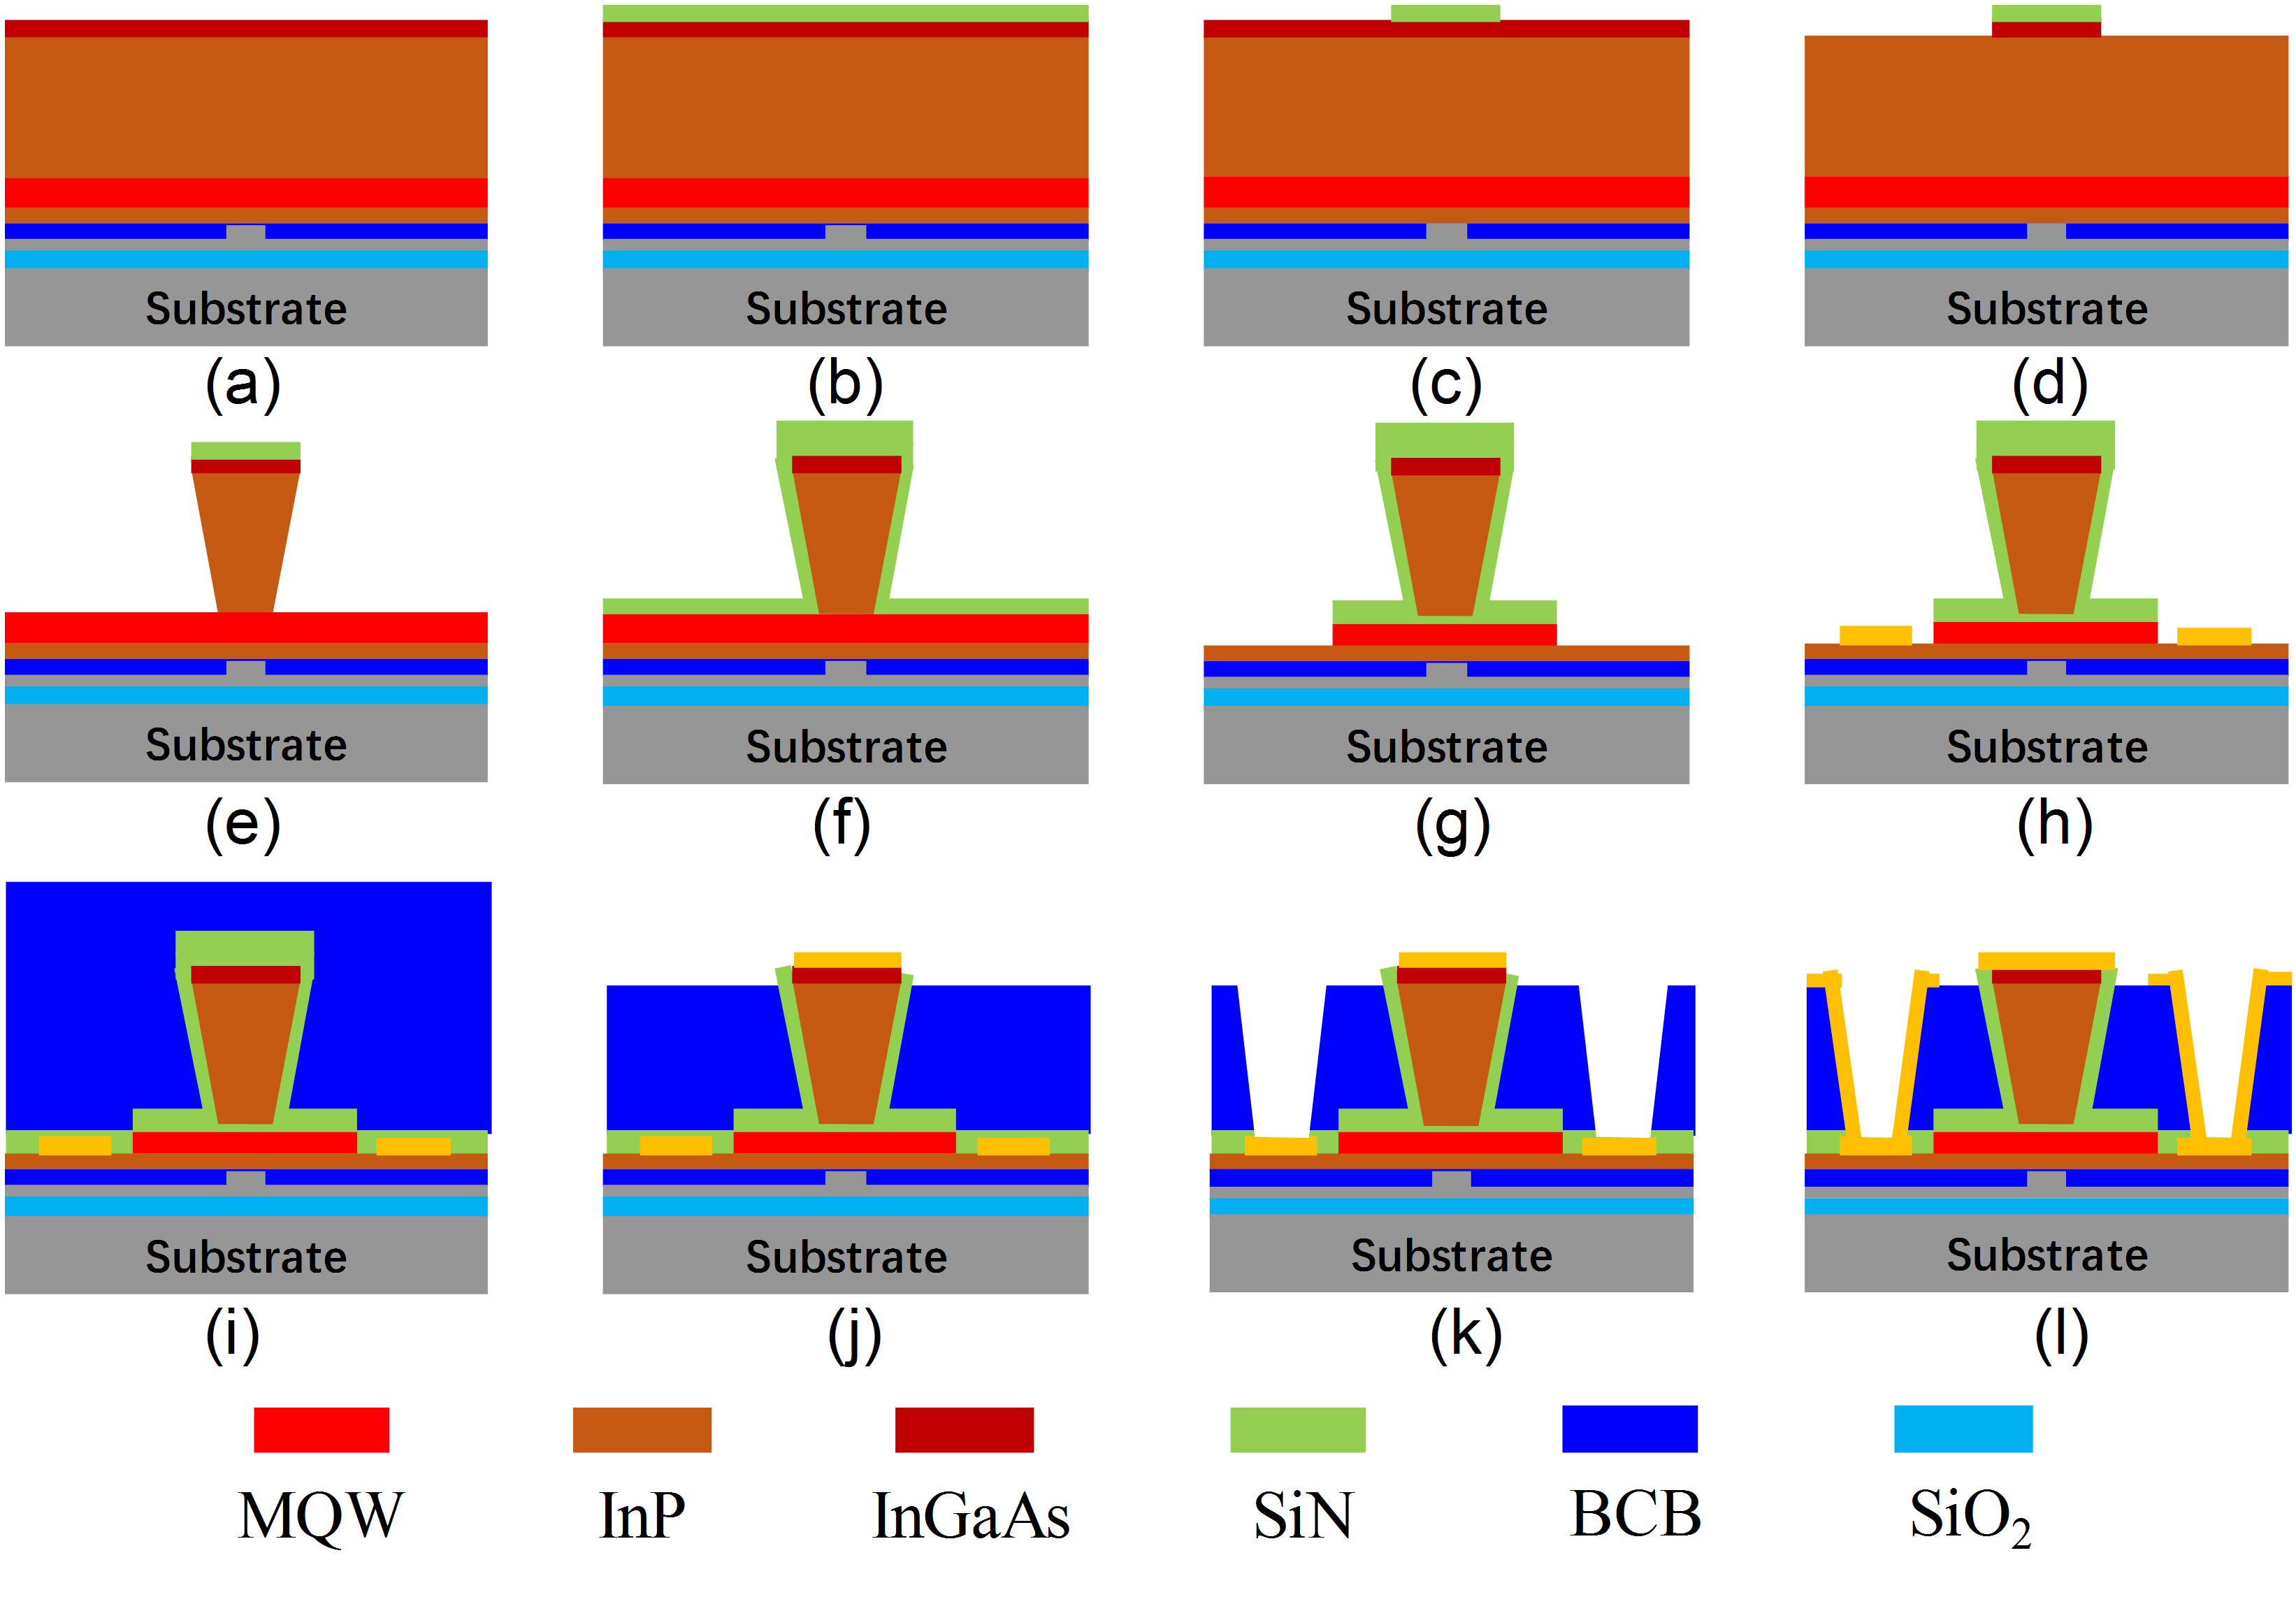
\includegraphics[width=\textwidth]{../Pictures/laser_fab.jpg}};
	\begin{scope}[x={(image.south east)},y={(image.north west)}]
		%\draw[help lines,xstep=.1,ystep=.1] (0,0) grid (1,1); %参考线绘制
		\only<2>{\draw[red,ultra thick,rounded corners] (0.79,0.5) rectangle (1,0.75);}
		\only<3>{\fill [draw=none, fill=white, fill opacity=0.9] (image.north west) -- (image.north east) -- (image.south east) -- (image.south west) -- (image.north west) -- cycle;
				 \node[anchor=center,inner sep=0](image1) at (image.center) {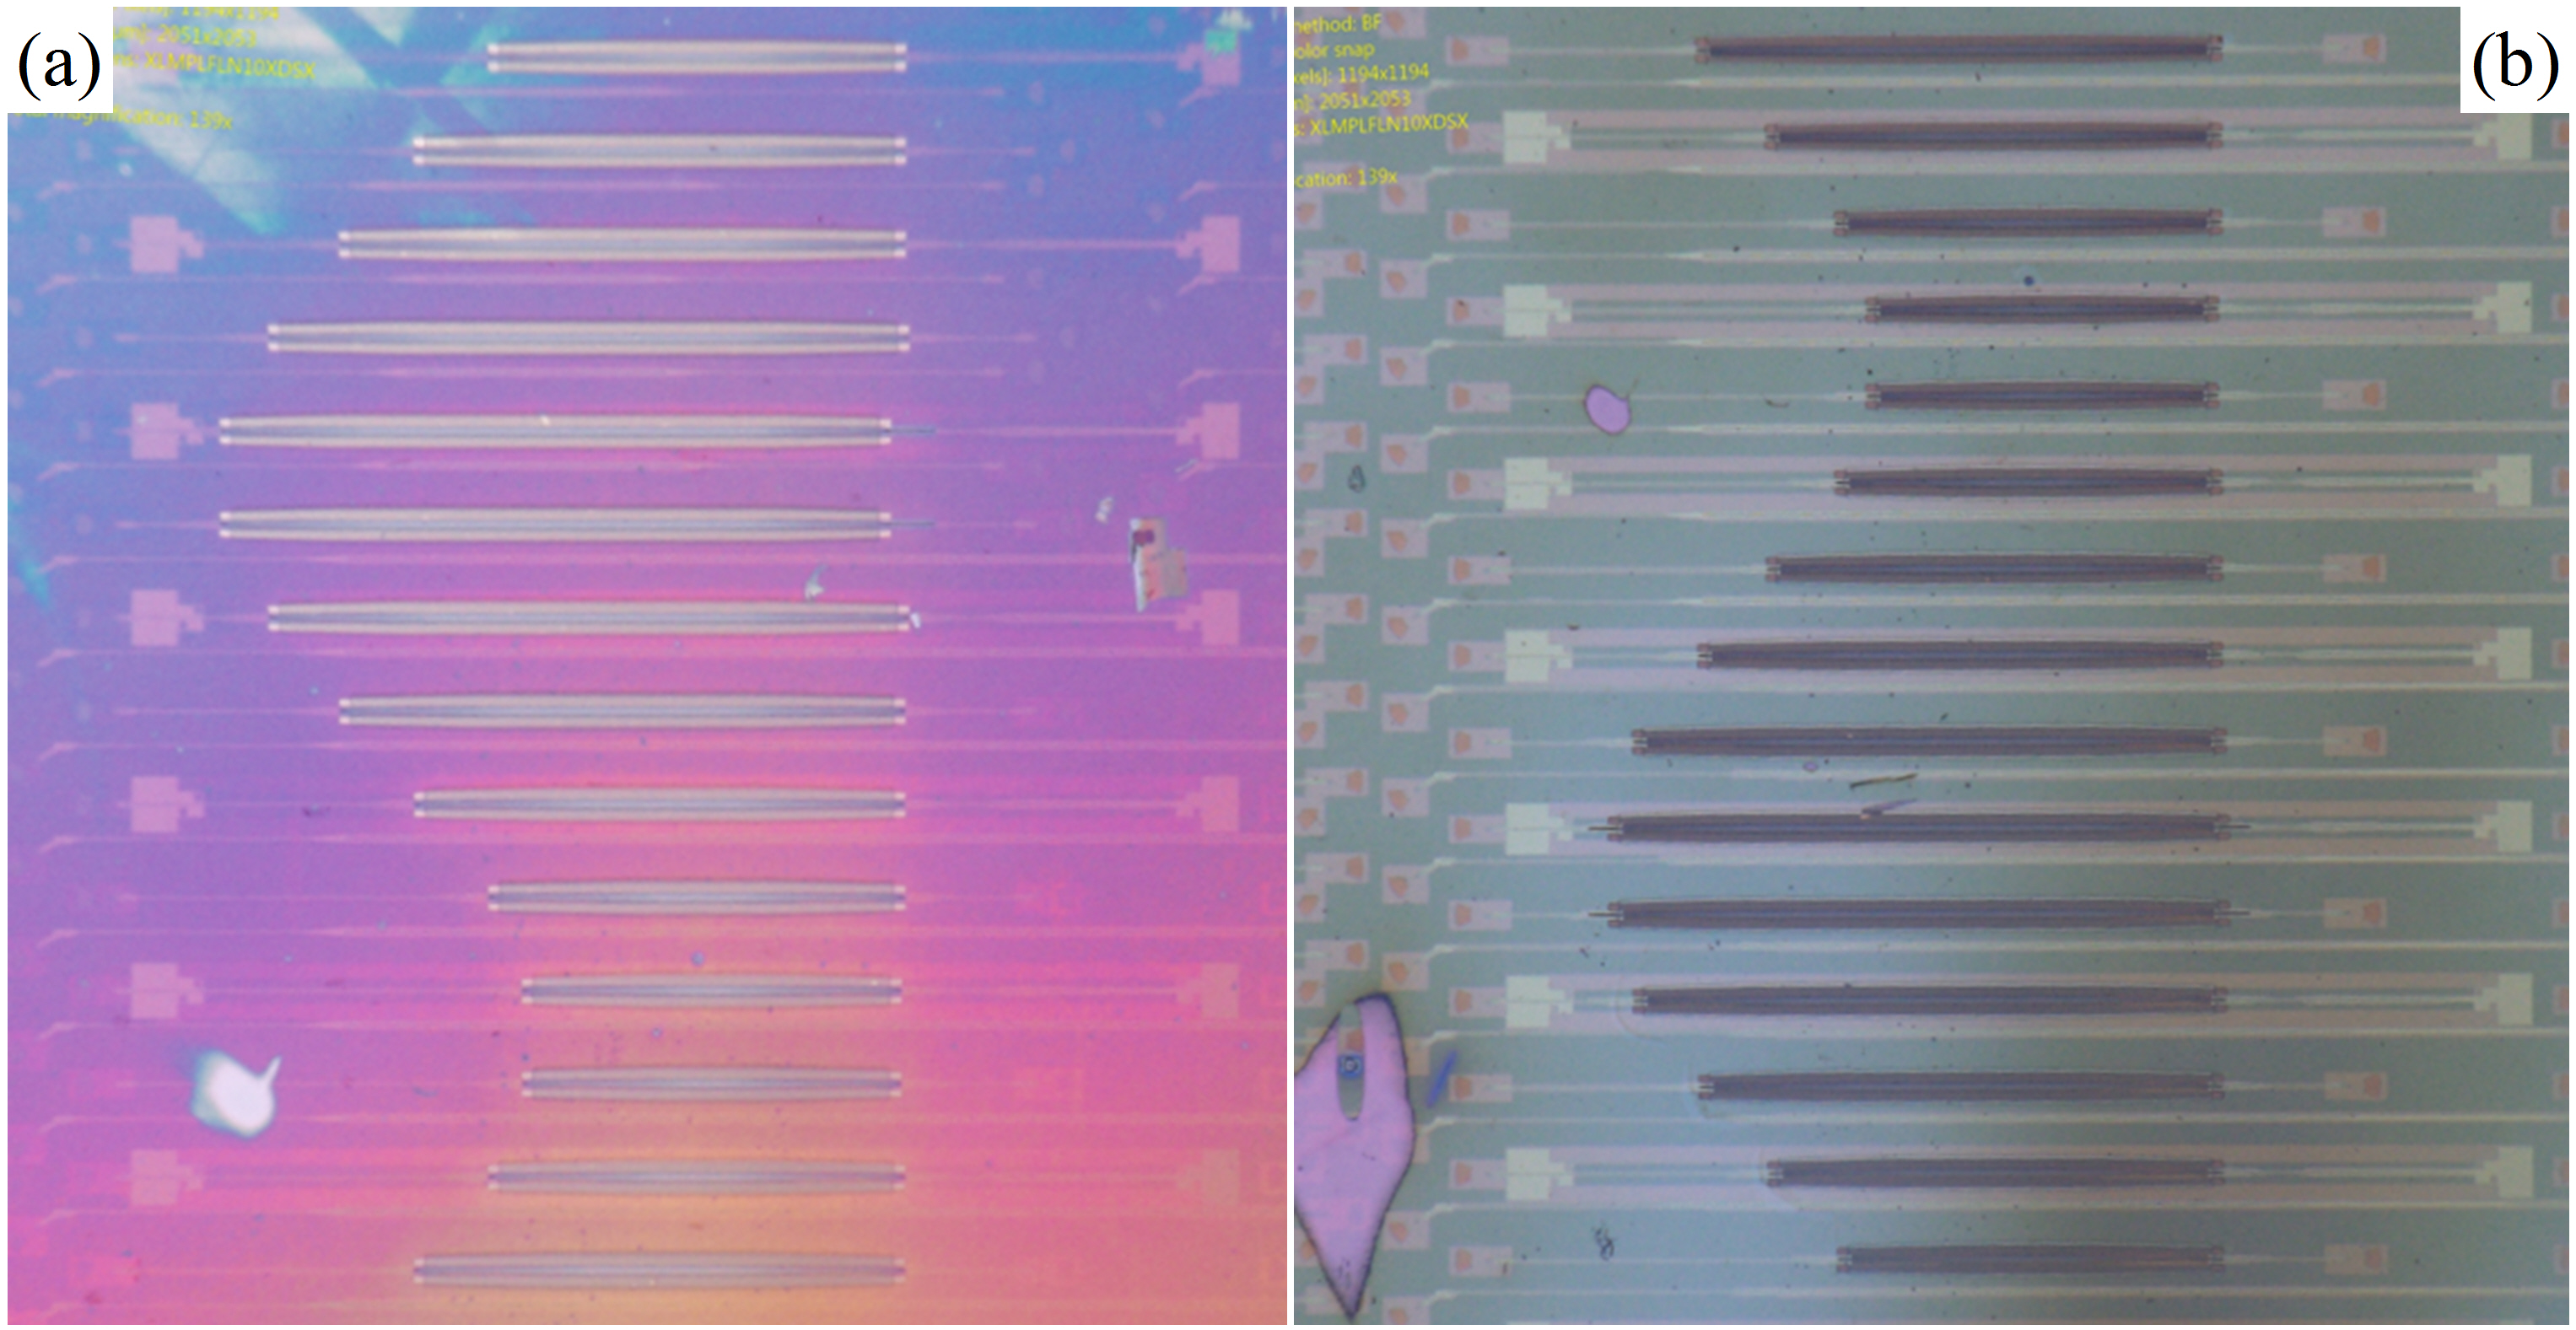
\includegraphics[width=0.7\textwidth]{../Pictures/laser_island.jpg}};
				 \node[anchor = north,inner sep=4pt,font=\bfseries,xshift=-1.8cm] at (image1.south) {n-InP未腐蚀完};
				 \node[anchor = north,inner sep=4pt,font=\bfseries,xshift=1.8cm] at (image1.south) {n-InP腐蚀完};}
		\only<4>{\draw[red,ultra thick,rounded corners] (0.26,0.19) rectangle (0.48,0.4);}
		\only<5>{\fill [draw=none, fill=white, fill opacity=0.9] (image.north west) -- (image.north east) -- (image.south east) -- (image.south west) -- (image.north west) -- cycle;
			\node[anchor=center,inner sep=0](image1) at (image.center) {\includegraphics[width=0.7\textwidth]{../Pictures/laser_cut.jpg}};}
	\end{scope}
\end{tikzpicture}
\end{frame}

\begin{frame}{器件的制作}
\centering
\begin{tikzpicture}
\node[anchor=south west,inner sep=0] (image) at (0,0) {\includegraphics[width=\textwidth]{../Pictures/laser_fabricationresult.jpg}};
\begin{scope}[x={(image.south east)},y={(image.north west)}]
%\draw[help lines,xstep=.1,ystep=.1] (0,0) grid (1,1); %参考线绘制
\end{scope}
\end{tikzpicture}
\end{frame}

\begin{frame}{静态性能测试——金属电极退火}
\centering
\begin{tikzpicture}
\node[anchor=south west,inner sep=0] (image) at (0,0) {\hspace{-0.5cm}\includegraphics[width=0.8\textwidth]{../Pictures/laser_annealing.jpg}};
\begin{scope}[x={(image.south east)},y={(image.north west)}]
%\draw[help lines,xstep=.1,ystep=.1] (0,0) grid (1,1); %参考线绘制
\node[anchor = east,align = left,red,draw,font=\bfseries] at (0.5,0.62) {利用焦耳热对\\电极进行退火};
\end{scope}
\end{tikzpicture}
\end{frame}

\begin{frame}{IV曲线}
\centering
\begin{tikzpicture}
\node[anchor=south west,inner sep=0] (image) at (0,0) {\includegraphics[width=\textwidth]{../Pictures/laser_IV.jpg}};
\begin{scope}[x={(image.south east)},y={(image.north west)}]
%\draw[help lines,xstep=.1,ystep=.1] (0,0) grid (1,1); %参考线绘制
\end{scope}
\end{tikzpicture}
\end{frame}

\begin{frame}{PI曲线}
\centering
\begin{tikzpicture}
\node[anchor=south west,inner sep=0] (image) at (0,0) {\includegraphics[width=\textwidth]{../Pictures/laser_PI.jpg}};
\begin{scope}[x={(image.south east)},y={(image.north west)}]
%\draw[help lines,xstep=.1,ystep=.1] (0,0) grid (1,1); %参考线绘制
\end{scope}
\end{tikzpicture}
\end{frame}

\begin{frame}{自脉冲信号}
\centering
\begin{tikzpicture}
\only<1>{\node[anchor=south west,inner sep=0] (image) at (0,0) {\includegraphics[width=0.7\textwidth]{./Pictures/setuposcillation.jpg}};}
\only<2>{\node[anchor=south west,inner sep=0] (image) at (0,0) {\includegraphics[width=0.9\textwidth]{./Pictures/equipment.jpg}};}
\only<3>{\node[anchor=south west,inner sep=0] (image) at (0,0) {\includegraphics[width=0.7\textwidth]{../Pictures/laser_lock1.jpg}};}
\only<4>{\node[anchor=south west,inner sep=0] (image) at (0,0) {\includegraphics[width=0.9\textwidth]{./Pictures/oscilation.jpg}};}
\begin{scope}[x={(image.south east)},y={(image.north west)}]
%\draw[help lines,xstep=.1,ystep=.1] (0,0) grid (1,1); %参考线绘制
\end{scope}
\end{tikzpicture}
\end{frame}

\begin{frame}{激光器光谱}
\centering
\begin{tikzpicture}
\node[anchor=south west,inner sep=0] (image) at (0,0) {\includegraphics[width=0.8\textwidth]{../Pictures/laser_spectrum.jpg}};
\node[anchor = north,inner sep=0pt,font=\bfseries,red,draw,xshift=-1.5cm,yshift=2cm] at (image.center) {拍频产生自脉冲};
\begin{scope}[x={(image.south east)},y={(image.north west)}]
%\draw[help lines,xstep=.1,ystep=.1] (0,0) grid (1,1); %参考线绘制
\end{scope}
\end{tikzpicture}
\end{frame}

%\begin{frame}{不同长度的激光器自脉冲电流组合}
%\centering
%\begin{tikzpicture}
%\node[anchor=south west,inner sep=0] (image) at (0,0) {\includegraphics[width=0.7\textwidth]{../Pictures/laser_combination.jpg}};
%\begin{scope}[x={(image.south east)},y={(image.north west)}]
%	%\draw[help lines,xstep=.1,ystep=.1] (0,0) grid (1,1); %参考线绘制
%	\node[anchor = center,inner sep=0pt,font=\bfseries,red,draw] at (0.28,0.96) {300 $\mu m$};
%	\node[anchor = center,inner sep=0pt,font=\bfseries,red,draw] at (0.78,0.96) {400 $\mu m$};
%	\node[anchor = center,inner sep=0pt,font=\bfseries,red,draw] at (0.28,0.48) {500 $\mu m$};
%	\node[anchor = center,inner sep=0pt,font=\bfseries,red,draw] at (0.78,0.48) {All together};
%\end{scope}
%\end{tikzpicture}
%\end{frame}

\begin{frame}{自脉冲频率与电流的关系}
\centering
\begin{tikzpicture}
\node[anchor=south west,inner sep=0] (image) at (0,0) {\includegraphics[width=0.8\textwidth]{../Pictures/laser_self_pulsation.jpg}};
\begin{scope}[x={(image.south east)},y={(image.north west)}]
%\draw[help lines,xstep=.1,ystep=.1] (0,0) grid (1,1); %参考线绘制
\end{scope}
\end{tikzpicture}
\end{frame}

\begin{frame}{自脉冲频率与温度的关系}
\centering
\begin{tikzpicture}
\node[anchor=south west,inner sep=0] (image) at (0,0) {\includegraphics[width=0.7\textwidth]{../Pictures/laser_temperature.jpg}};
\begin{scope}[x={(image.south east)},y={(image.north west)}]
%\draw[help lines,xstep=.1,ystep=.1] (0,0) grid (1,1); %参考线绘制
\end{scope}
\end{tikzpicture}
\end{frame}

\begin{frame}{自脉冲频率锁定}
\centering
\begin{tikzpicture}
\node[anchor=south west,inner sep=0] (image) at (0,0) {\includegraphics[width=\textwidth]{../Pictures/laser_lock.jpg}};
\begin{scope}[x={(image.south east)},y={(image.north west)}]
%\draw[help lines,xstep=.1,ystep=.1] (0,0) grid (1,1); %参考线绘制
\end{scope}
\end{tikzpicture}
\end{frame}

\begin{frame}{自脉冲DFB激光器的调制性能}
	\begin{columns}
		\begin{column}[c]{0.45\textwidth}
			\begin{tikzpicture}
			\node[anchor=south west,inner sep=0] (image) at (0,0) {\includegraphics[width=\textwidth]{../Pictures/laser_ppr_structure.jpg}};
			\begin{scope}[x={(image.south east)},y={(image.north west)}]
			%\draw[help lines,xstep=.1,ystep=.1] (0,0) grid (1,1); %参考线绘制
			\end{scope}
			\end{tikzpicture}
		\end{column}	
		\begin{column}[c]{0.55\textwidth}
			\begin{tikzpicture}
			\node[anchor=south west,inner sep=0] (image) at (0,0) {\includegraphics[width=\textwidth]{../Pictures/laser_ppr.jpg}};
			\node[anchor = north east] at (image.south east) {\bfseries\tiny \emph{Wei W., Laser Physics Lett., 13(12)}};
			\begin{scope}[x={(image.south east)},y={(image.north west)}]
			%\draw[help lines,xstep=.1,ystep=.1] (0,0) grid (1,1); %参考线绘制
			\end{scope}
			\end{tikzpicture}	
		\end{column}
	\end{columns}
\end{frame}

\begin{frame}{调制带宽测试示意图}
\centering
\begin{tikzpicture}
\node[anchor=south west,inner sep=0] (image) at (0,0) {\includegraphics[width=0.8\textwidth]{../Pictures/laser_s21_setup.jpg}};
\begin{scope}[x={(image.south east)},y={(image.north west)}]
%\draw[help lines,xstep=.1,ystep=.1] (0,0) grid (1,1); %参考线绘制
\end{scope}
\end{tikzpicture}
\end{frame}

\begin{frame}{调制带宽测试示意图}
\centering
\begin{tikzpicture}
\node[anchor=south west,inner sep=0] (image) at (0,0) {\includegraphics[width=0.8\textwidth]{../Pictures/laser_s21.jpg}};
\begin{scope}[x={(image.south east)},y={(image.north west)}]
%\draw[help lines,xstep=.1,ystep=.1] (0,0) grid (1,1); %参考线绘制
\end{scope}
\end{tikzpicture}
\end{frame}

\begin{frame}{数据传输测试示意图}
\centering
\begin{tikzpicture}
\node[anchor=south west,inner sep=0] (image) at (0,0) {\includegraphics[width=\textwidth]{../Pictures/laser_data_transmission_setup.jpg}};
\begin{scope}[x={(image.south east)},y={(image.north west)}]
%\draw[help lines,xstep=.1,ystep=.1] (0,0) grid (1,1); %参考线绘制
\end{scope}
\end{tikzpicture}
\end{frame}

\begin{frame}{数据传输眼图}
\centering
\begin{tikzpicture}
\node[anchor=south west,inner sep=0] (image) at (0,0) {\includegraphics[width=0.8\textwidth]{../Pictures/laser_data_transmission.jpg}};
\node[anchor = north,inner sep=4pt,font=\bfseries] at (image.south) {45 Gbps NRZ数据传输眼图:(a)背靠背;(b)2 km光纤};
\begin{scope}[x={(image.south east)},y={(image.north west)}]
%\draw[help lines,xstep=.1,ystep=.1] (0,0) grid (1,1); %参考线绘制
\end{scope}
\end{tikzpicture}
\end{frame}

\begin{frame}{接收功率与误码率之间的关系}
\centering
\begin{tikzpicture}
\node[anchor=south west,inner sep=0] (image) at (0,0) {\includegraphics[width=0.7\textwidth]{../Pictures/laser_ber.jpg}};
\node[anchor = north,inner sep=4pt,font=\bfseries] at (image.south) {接收功率与误码率之间的关系};
\begin{scope}[x={(image.south east)},y={(image.north west)}]
%\draw[help lines,xstep=.1,ystep=.1] (0,0) grid (1,1); %参考线绘制
\end{scope}
\end{tikzpicture}
\end{frame}

\begin{frame}{小结}
\zihao{4}
\begin{itemize}
	\item 制作了两段式自脉冲DFB激光器,研究了自脉冲频率与电流和温度的关系
	\item 研究了自脉冲的频率锁定现象,最小的锁定功率-17~dBm
	\item 研究了利用自脉冲激光器提升激光器调制带宽的现象,实现了45~Gbps的数据传输速率
\end{itemize}
\end{frame}

\subsection{\mbox{EDG}光谱仪的设计优化与制作}
\frame{\tableofcontents[currentsubsection]}
\begin{frame}[t]{非色散红外吸收光谱法检测气体浓度系统}
\begin{block}{Beer-Lambert定律}
	Beer-Lambert定律是气体吸收领域最基本的定律,该定律描述的是一束单色平行光经过某种均匀混合的气体吸收后,其透射光强与入射光强之间的关系,即
	\begin{equation*}
		I_{t}(\upsilon) = I_{o}(\upsilon)exp(-\sigma_{ext}NL)
	\end{equation*}
\end{block}
\centering
\begin{tikzpicture}
\node[anchor=south west,inner sep=0] (image) at (0,0) {\includegraphics[width=0.8\textwidth]{../Pictures/edg_gas_equipment.jpg}};
\begin{scope}[x={(image.south east)},y={(image.north west)}]
%\draw[help lines,xstep=.1,ystep=.1] (0,0) grid (1,1); %参考线绘制
\end{scope}
\end{tikzpicture}
\end{frame}

\begin{frame}{片上光谱仪简介}
\centering
\begin{tikzpicture}
\node[anchor=south west,inner sep=0] (image) at (0,0) {\includegraphics[width=0.7\textwidth]{../Pictures/edg_background.jpg}};
\begin{scope}[x={(image.south east)},y={(image.north west)}]
	%\draw[help lines,xstep=.1,ystep=.1] (0,0) grid (1,1); %参考线绘制
	\node[anchor = south,inner sep=0pt,font=\bfseries,red] at (0.27,0.7) {光栅型};
	\node[anchor = south,inner sep=0pt,font=\bfseries,red] at (0.75,0.7) {数字平面全息型};
	\node[anchor = south,inner sep=0pt,font=\bfseries,red] at (0.5,0.4) {谐振腔型};
	\node[anchor = south,inner sep=0pt,font=\bfseries,red] at (0.27,0.03) {光子晶体型};
	\node[anchor = south,inner sep=0pt,font=\bfseries,red] at (0.75,0.03) {随机散射光谱仪};
\end{scope}
\end{tikzpicture}
\end{frame}

\begin{frame}{不同类型光谱仪特性总结}
\centering{不同类型光谱仪特性总结}
\begin{table}[h]
		\centering
		\zihao{6}
		\begin{tabular}[t]{|ccc|}
			\hline
			\textbf{光谱仪类型} & \textbf{优点} & \textbf{缺点}  \\
			\hline
			光栅型光谱仪(AWG,EDG)&设计成熟、工艺方便&尺寸较大\\
			\hline
			数字平面全息光谱仪&分辨率较高&损耗较大,灵敏度受限\\
			\hline
			谐振腔型光谱仪&分辨率高,尺寸较小&对工艺敏感,需后期校正\\
			\hline
			光子晶体光谱仪&分辨率高,尺寸较小&只能用来探测单一的谱线\\
			\hline
			随机散射光谱仪&分辨率高,波长范围可切换&需要专门的算法优化\\
			\hline
		\end{tabular}
\end{table}
\end{frame}

\begin{frame}{\mbox{EDG}光谱仪的设计优化}
\centering
\begin{tikzpicture}
\node[anchor=south west,inner sep=0] (image) at (0,0) {\includegraphics[width=\textwidth]{../Pictures/edg_refractive_index.jpg}};
\begin{scope}[x={(image.south east)},y={(image.north west)}]
%\draw[help lines,xstep=.1,ystep=.1] (0,0) grid (1,1); %参考线绘制
\node[anchor=west,inner sep=0,red] at (0.14,0.26) {\bm{$\dfrac{P_{1\rightarrow2}}{P_{1}}=\frac{1}{(\Delta\beta /2\kappa)^2+1}sin^2\sqrt{(\Delta \beta/2)^2 +\kappa^2}L$}};
\end{scope}
\end{tikzpicture}
\end{frame}

\begin{frame}{波导阵列\mbox{3D}示意图}
\centering
\begin{tikzpicture}
\node[anchor=south west,inner sep=0] (image) at (0,0) {\includegraphics[width=\textwidth]{../Pictures/edg_dpwg.jpg}};
\begin{scope}[x={(image.south east)},y={(image.north west)}]
%\draw[help lines,xstep=.1,ystep=.1] (0,0) grid (1,1); %参考线绘制
\end{scope}
\end{tikzpicture}
\end{frame}

\begin{frame}{波导阵列仿真}
\centering
\begin{tikzpicture}
\node[anchor=south west,inner sep=0] (image) at (0,0) {\includegraphics[width=\textwidth]{../Pictures/edg_taper_xtalk.jpg}};
\begin{scope}[x={(image.south east)},y={(image.north west)}]
%\draw[help lines,xstep=.1,ystep=.1] (0,0) grid (1,1); %参考线绘制
\end{scope}
\end{tikzpicture}
\end{frame}

\begin{frame}{\mbox{EDG}光谱仪结构示意图}
\centering
\begin{tikzpicture}
\node[anchor=south west,inner sep=0] (image) at (0,0) {\includegraphics[width=\textwidth]{../Pictures/edg_layout.jpg}};
\begin{scope}[x={(image.south east)},y={(image.north west)}]
%\draw[help lines,xstep=.1,ystep=.1] (0,0) grid (1,1); %参考线绘制
\node[anchor=south east,inner sep=0] at (1,0) {\includegraphics[width=0.27\textwidth]{../Pictures/edg_dbr_loss.jpg}};
\node[anchor=center,inner sep=0] (A) at (0.52,0.5) {\includegraphics[width=0.32\textwidth]{./Pictures/twostigmaticpoints.jpg}};
\node[anchor = south east,inner sep=0,font=\tiny, scale =0.8] at (A.south east) {\bfseries \emph{Horst F., Photon. Technol. Lett., 21(23)}};
\end{scope}
\end{tikzpicture}
\end{frame}

%\begin{frame}{\mbox{EDG}光谱仪仿真}
%\centering
%\begin{tikzpicture}
%\node[anchor=south west,inner sep=0] (image) at (0,0) {\includegraphics[width=0.7\textwidth]{../Pictures/edg_diffraction_method.jpg}};
%\begin{scope}[x={(image.south east)},y={(image.north west)}]
%%\draw[help lines,xstep=.1,ystep=.1] (0,0) grid (1,1); %参考线绘制
%%\node[anchor=south east,inner sep=0] at (1,0) {\includegraphics[width=0.27\textwidth]{../Pictures/edg_dbr_loss.jpg}};
%%\node[anchor=center,inner sep=0] (A) at (0.52,0.5) {\includegraphics[width=0.32\textwidth]{./Pictures/twostigmaticpoints.jpg}};
%%\node[anchor = south east,inner sep=0,font=\tiny, scale =0.8] at (A.south east) {\bfseries \emph{Horst F., Photon. Technol. Lett. 21(23)}};
%\end{scope}
%\end{tikzpicture}
%\begin{equation*}
%U(x_{1})=\dfrac{je^{-jkz}e^{-jkx_{0}^2/2 z}}{\lambda z}\int_{-\infty}^{\infty}U(x_{0})e^{-jkx_{0}^{2}/2z}e^{-j2\pi x_{1}x_{0}/\lambda z}\,dx_{0}
%\end{equation*}
%\end{frame}

\begin{frame}{\mbox{EDG}光谱仪仿真}
\centering
\begin{tikzpicture}
\node[anchor=south west,inner sep=0] (image) at (0,0) {\includegraphics[width=0.9\textwidth]{../Pictures/edg_simulated_spectrum.jpg}};
\begin{scope}[x={(image.south east)},y={(image.north west)}]
%\draw[help lines,xstep=.1,ystep=.1] (0,0) grid (1,1); %参考线绘制
%\node[anchor=south east,inner sep=0] at (1,0) {\includegraphics[width=0.27\textwidth]{../Pictures/edg_dbr_loss.jpg}};
%\node[anchor=center,inner sep=0] (A) at (0.52,0.5) {\includegraphics[width=0.32\textwidth]{./Pictures/twostigmaticpoints.jpg}};
%\node[anchor = south east,inner sep=0,font=\tiny, scale =0.8] at (A.south east) {\bfseries \emph{Horst F., Photon. Technol. Lett. 21(23)}};
\end{scope}
\end{tikzpicture}
\end{frame}

\begin{frame}{\mbox{EDG}光谱仪的制作}
\centering
\begin{tikzpicture}
\node[anchor=south west,inner sep=0] (image) at (0,0) {\includegraphics[width=0.9\textwidth]{../Pictures/edg_fabrication.jpg}};
\begin{scope}[x={(image.south east)},y={(image.north west)}]
%\draw[help lines,xstep=.1,ystep=.1] (0,0) grid (1,1); %参考线绘制
%\node[anchor=south east,inner sep=0] at (1,0) {\includegraphics[width=0.27\textwidth]{../Pictures/edg_dbr_loss.jpg}};
%\node[anchor=center,inner sep=0] (A) at (0.52,0.5) {\includegraphics[width=0.32\textwidth]{./Pictures/twostigmaticpoints.jpg}};
%\node[anchor = south east,inner sep=0,font=\tiny, scale =0.8] at (A.south east) {\bfseries \emph{Horst F., Photon. Technol. Lett. 21(23)}};
\end{scope}
\end{tikzpicture}
\end{frame}

\begin{frame}{\mbox{EBL}描边法}
\centering
\begin{tikzpicture}
\node[anchor=south west,inner sep=0] (image) at (0,0) {\includegraphics[width=0.9\textwidth]{../Pictures/edg_pattern_mode.jpg}};
\node[anchor = north,inner sep=4pt,font=\bfseries,xshift=-2.5cm] at (image.south) {拼接模式};
\node[anchor = north,inner sep=4pt,font=\bfseries,xshift=2.5cm] at (image.south) {连续模式};
\begin{scope}[x={(image.south east)},y={(image.north west)}]
%\draw[help lines,xstep=.1,ystep=.1] (0,0) grid (1,1); %参考线绘制
%\node[anchor=south east,inner sep=0] at (1,0) {\includegraphics[width=0.27\textwidth]{../Pictures/edg_dbr_loss.jpg}};
%\node[anchor=center,inner sep=0] (A) at (0.52,0.5) {\includegraphics[width=0.32\textwidth]{./Pictures/twostigmaticpoints.jpg}};
%\node[anchor = south east,inner sep=0,font=\tiny, scale =0.8] at (A.south east) {\bfseries \emph{Horst F., Photon. Technol. Lett. 21(23)}};
\end{scope}
\end{tikzpicture}
\end{frame}

\begin{frame}{\mbox{EBL}描边法}
\centering
\begin{tikzpicture}
\node[anchor=south west,inner sep=0] (image) at (0,0) {\includegraphics[width=\textwidth]{../Pictures/edg_misalignment.jpg}};
\begin{scope}[x={(image.south east)},y={(image.north west)}]
%\draw[help lines,xstep=.1,ystep=.1] (0,0) grid (1,1); %参考线绘制
%\node[anchor=south east,inner sep=0] at (1,0) {\includegraphics[width=0.27\textwidth]{../Pictures/edg_dbr_loss.jpg}};
%\node[anchor=center,inner sep=0] (A) at (0.52,0.5) {\includegraphics[width=0.32\textwidth]{./Pictures/twostigmaticpoints.jpg}};
%\node[anchor = south east,inner sep=0,font=\tiny, scale =0.8] at (A.south east) {\bfseries \emph{Horst F., Photon. Technol. Lett. 21(23)}};
\end{scope}
\end{tikzpicture}
\end{frame}

\begin{frame}{\mbox{EBL}描边法}
\centering
\begin{tikzpicture}
\node[anchor=south west,inner sep=0] (image) at (0,0) {\includegraphics[width=0.5\textwidth]{../Pictures/edg_fbms.jpg}};
\node[anchor = north,inner sep=4pt,font=\bfseries,yshift=2cm,red] at (image.center) {FBMS line};
\node[anchor = south,inner sep=4pt,font=\bfseries,red,yshift=0.3cm] at (image.south) {FBMS Area};
\begin{scope}[x={(image.south east)},y={(image.north west)}]
%\draw[help lines,xstep=.1,ystep=.1] (0,0) grid (1,1); %参考线绘制
%\node[anchor=south east,inner sep=0] at (1,0) {\includegraphics[width=0.27\textwidth]{../Pictures/edg_dbr_loss.jpg}};
%\node[anchor=center,inner sep=0] (A) at (0.52,0.5) {\includegraphics[width=0.32\textwidth]{./Pictures/twostigmaticpoints.jpg}};
%\node[anchor = south east,inner sep=0,font=\tiny, scale =0.8] at (A.south east) {\bfseries \emph{Horst F., Photon. Technol. Lett. 21(23)}};
\end{scope}
\end{tikzpicture}
\end{frame}

\begin{frame}{\mbox{EBL}描边法}
\centering
\begin{tikzpicture}
\node[anchor=south west,inner sep=0] (image) at (0,0) {\includegraphics[width=0.9\textwidth]{../Pictures/edg_miaobian.jpg}};
\begin{scope}[x={(image.south east)},y={(image.north west)}]
%\draw[help lines,xstep=.1,ystep=.1] (0,0) grid (1,1); %参考线绘制
%\node[anchor=south east,inner sep=0] at (1,0) {\includegraphics[width=0.27\textwidth]{../Pictures/edg_dbr_loss.jpg}};
%\node[anchor=center,inner sep=0] (A) at (0.52,0.5) {\includegraphics[width=0.32\textwidth]{./Pictures/twostigmaticpoints.jpg}};
%\node[anchor = south east,inner sep=0,font=\tiny, scale =0.8] at (A.south east) {\bfseries \emph{Horst F., Photon. Technol. Lett. 21(23)}};
\end{scope}
\end{tikzpicture}
\end{frame}

%\begin{frame}{\mbox{EBL}描边法}
%\centering
%\begin{tikzpicture}
%\node[anchor=south west,inner sep=0] (image) at (0,0) {\includegraphics[width=0.9\textwidth]{../Pictures/edg_ripple.jpg}};
%\begin{scope}[x={(image.south east)},y={(image.north west)}]
%%\draw[help lines,xstep=.1,ystep=.1] (0,0) grid (1,1); %参考线绘制
%%\node[anchor=south east,inner sep=0] at (1,0) {\includegraphics[width=0.27\textwidth]{../Pictures/edg_dbr_loss.jpg}};
%%\node[anchor=center,inner sep=0] (A) at (0.52,0.5) {\includegraphics[width=0.32\textwidth]{./Pictures/twostigmaticpoints.jpg}};
%%\node[anchor = south east,inner sep=0,font=\tiny, scale =0.8] at (A.south east) {\bfseries \emph{Horst F., Photon. Technol. Lett. 21(23)}};
%\end{scope}
%\end{tikzpicture}
%\end{frame}

\begin{frame}{\mbox{EDG}光谱仪制作结果}
\centering
\begin{tikzpicture}
\node[anchor=south west,inner sep=0] (image) at (0,0) {\includegraphics[width=0.6\textwidth]{../Pictures/edg_fabrication_sem.jpg}};
\begin{scope}[x={(image.south east)},y={(image.north west)}]
%\draw[help lines,xstep=.1,ystep=.1] (0,0) grid (1,1); %参考线绘制
%\node[anchor=south east,inner sep=0] at (1,0) {\includegraphics[width=0.27\textwidth]{../Pictures/edg_dbr_loss.jpg}};
%\node[anchor=center,inner sep=0] (A) at (0.52,0.5) {\includegraphics[width=0.32\textwidth]{./Pictures/twostigmaticpoints.jpg}};
%\node[anchor = south east,inner sep=0,font=\tiny, scale =0.8] at (A.south east) {\bfseries \emph{Horst F., Photon. Technol. Lett. 21(23)}};
\end{scope}
\end{tikzpicture}
\end{frame}

\begin{frame}{\mbox{EDG}光谱仪的测试}
\centering
\begin{tikzpicture}
\node[anchor=south west,inner sep=0] (image) at (0,0) {\includegraphics[width=0.7\textwidth]{../Pictures/edg_setup.jpg}};
\begin{scope}[x={(image.south east)},y={(image.north west)}]
%\draw[help lines,xstep=.1,ystep=.1] (0,0) grid (1,1); %参考线绘制
%\node[anchor=south east,inner sep=0] at (1,0) {\includegraphics[width=0.27\textwidth]{../Pictures/edg_dbr_loss.jpg}};
%\node[anchor=center,inner sep=0] (A) at (0.52,0.5) {\includegraphics[width=0.32\textwidth]{./Pictures/twostigmaticpoints.jpg}};
%\node[anchor = south east,inner sep=0,font=\tiny, scale =0.8] at (A.south east) {\bfseries \emph{Horst F., Photon. Technol. Lett. 21(23)}};
\end{scope}
\end{tikzpicture}
\end{frame}

\begin{frame}{\mbox{EDG}光谱仪的测试}
\centering
\begin{tikzpicture}
\node[anchor=south west,inner sep=0] (image) at (0,0) {\includegraphics[width=0.8\textwidth]{../Pictures/edg_transmission.jpg}};
\begin{scope}[x={(image.south east)},y={(image.north west)}]
%\draw[help lines,xstep=.1,ystep=.1] (0,0) grid (1,1); %参考线绘制
%\node[anchor=south east,inner sep=0] at (1,0) {\includegraphics[width=0.27\textwidth]{../Pictures/edg_dbr_loss.jpg}};
%\node[anchor=center,inner sep=0] (A) at (0.52,0.5) {\includegraphics[width=0.32\textwidth]{./Pictures/twostigmaticpoints.jpg}};
%\node[anchor = south east,inner sep=0,font=\tiny, scale =0.8] at (A.south east) {\bfseries \emph{Horst F., Photon. Technol. Lett. 21(23)}};
\end{scope}
\end{tikzpicture}
\end{frame}

\begin{frame}{\mbox{EDG}光谱仪的测试}
\centering{最近基于\mbox{EDG}的光谱仪性能比较,中心波长均为1550~$nm$}
\begin{table}[h]
	\centering
	\zihao{6}
	\begin{tabular}[t]{|c|c|c|c|c|}
		\hline
		\textbf{Reference} & This work & Pommarede & Xie & Ryckeboer \\
		\hline
		\textbf{Platform} & 220~$nm$~SOI & 300~$nm$~SOI & 300~$nm$~SiN & 220~$nm$~SOI\\
		\hline
		\textbf{Insertion loss (dB)} & 6.9 & 1.8 & 1.39 & 5\\
		\hline
		\textbf{Non-uniformity (dB)} & 1.7 & 0.5 & 1.2 & \~{}1\\
		\hline
		\textbf{Crosstalk (dB)} & -4.3 & -15 & -30 & -16\\
		\hline
		\textbf{Channel spacing (nm)} & 0.5 & 0.8 & 5 & 3.2\\
		\hline
		\textbf{Resolution ($\pmb{\lambda/\Delta\lambda}$)} & \textbf{{\color{red}5571}} & 4822 & 1300 & Not given \\
		\hline
		\textbf{Number of channels} & 20 & 16 & 5 & 8 \\
		\hline
		\textbf{Footprint ($\pmb{mm^{2}}$)} & 9 & 2.6 & 3 & 0.56\\
		\hline
	\end{tabular}
\end{table}
\vspace{1cm}
\flushright\tiny\bfseries\emph
{Pommarede X., Photon. Technol. Lett., 29(6)\\Xie S., Photon. IEEE Photon. J., 10(6)\\Ryckeboer E., Opt. Exp., 21(5)}
\end{frame}

\begin{frame}{小结}
\zihao{4}
\begin{itemize}
	\item 利用自脉冲激光器的双波长特性与光谱仪结合设计了一套气体浓度检测系统
	\item 利用密集阵列波导优化了片上\mbox{EDG}光谱仪的光谱分辨率
	\item 针对\mbox{EBL}加工尺寸较大结构的限制,采用了描边法完成了器件的部分加工
\end{itemize}
\end{frame}

\section{总结与展望}
\frame{\tableofcontents[currentsection]}
\begin{frame}{总结}
\begin{itemize}
	\item 研究了\mbox{SOI}刻蚀深度与颜色的对应关系,可以利用颜色比较法检测硅层厚度。
	\item 提出了一种混合集成自脉冲激光器的方案,利用两段DFB结构,实现了自脉冲频率连续可调的激光器。
	\item 发现了自脉冲激光器的微波频率锁定现象,锁定功率最小为-17 dBm,可以实现带宽小于10~Hz的光学微波信号。
	\item 利用自脉冲激光器的光子共振现象提升了直调带宽,实现了45~Gbps的数据传输速率。
	\item 设计了一套利用自脉冲激光器与光谱仪结合的气体浓度检测系统。
	\item 利用密集阵列波导优化了EDG光谱仪的通道间隔达到0.5 $nm$,可以实现121通道的设计。
\end{itemize}
\end{frame}

\begin{frame}{展望}
\zihao{5}
\begin{itemize}
	\item 现阶段颜色比较法来测定硅层厚度只能通过肉眼来确定,往往不够准确且受个人的影响比较大,可以利用计算机通过相关算法进行颜色匹配以增加可靠性。且目前该方法只适用于大面积硅层情况下,之后可以结合显微镜,将软件集成到显微镜中帮助判断局部硅层的厚度。
	\item 之前由于设备的限制,该激光器产生的微波信号只测到40 GHz,可以进一步研究该激光器在太赫兹波产生方面的应用。
	\item 自脉冲激光器的结构参数还可以进一步优化来提升调制带宽。
	\item 对于EBL加工的通道限制问题,可以使用流片工艺进行解决,得到设计的121通道的EDG光谱仪。而且利用了流片工艺之后,通道的均匀性可以进一步提升。现阶段制作的光谱仪没有集成探测器,还需要外接探测器进行测量,之后还可以在每个通道输出口集成片上探测器,以实现真正的片上光谱仪。
\end{itemize}
\end{frame}


\begin{frame}
\frametitle{博士期间发表的论文}
\zihao{-5}
\begin{columns}
	\column{\dimexpr\paperwidth-20pt}
	\begin{enumerate}
		\item \textbf{K. Ma}, K. Chen, N. Zhu, L. Liu, and S. He. High-resolution compact on-chip spectrometer based on an echelle grating with densely packed waveguide array. IEEE Photonics Journal, 11(1): 1-7, 2019.
		\item \textbf{K. Ma}, M. Shahin, A. Abbassi, G. Roelkens, and G. Morthier. Demonstration of InP-on-Si self-pulsating DFB laser diodes for optical microwave generation. IEEE Photonics Journal, 9(4): 1-8, 2017.
		\item M. Shahin, \textbf{K. Ma}, A. Abbassi, G. Roelkens, and G. Morthier. 45 Gb/s direct modulation of two-section InP-on-Si DFB laser Diodes. IEEE Photonics Technology Letters, 30(8):685-687, 2018.
		\item Q. Huang, \textbf{K. Ma}, and S. He. Experimental Demonstration of Single Mode-Splitting in Microring With Bragg Gratings. IEEE Photonics Thechnology Letters, 27(13): 1402-1405, 2015.
	\end{enumerate}
\end{columns}

\end{frame}

\begin{frame}
\frametitle{致谢}
\begin{itemize}
	\item 感谢我的导师何赛灵教授!
	\item 感谢戴道锌教授、时尧成教授、\mbox{\bfseries Geert Morthier}教授的无私帮助!
	\item 感谢胡鑫松师傅、实验员陈辉,金姐、吴姐等\mbox{\bfseries COER}工作人员的关怀!
	\item 感谢\mbox{\bfseries PLC}、\mbox{\bfseries COER}等的同学们的帮助与陪伴!
	\item 感谢女友卢梦娇和父母的支持!
	\item 感谢答辩委员会的各位老师!
\end{itemize}
\end{frame}

\begin{frame}
	\centering
	\includegraphics[width=0.65\textwidth]{./Pictures/questionandanswer.jpg}
\end{frame}

\end{document}

